%============================================================================
% tento soubor pouzijte jako zaklad
% (c) 2008 Michal Bidlo
% E-mail: bidlom AT fit vutbr cz
%============================================================================
% kodovaní: UTF-8 (zmena prikazem iconv, recode nebo cstocs)
%----------------------------------------------------------------------------
% zpracování: make, make pdf, make clean
%============================================================================
% Šablonu upravil: Ing. Jaroslav Dytrych, idytrych@fit.vutbr.cz
%============================================================================
\documentclass[]{fitthesis} % bez zadání - pro začátek práce, aby nebyl problém s překladem
%\documentclass[zadani]{fitthesis} % odevzdani do wisu - odkazy jsou barevné
%\documentclass[zadani,print]{fitthesis} % pro tisk - odkazy jsou černé
%\documentclass[english,print]{fitthesis} % pro tisk - odkazy jsou černé
% * Je-li prace psana v anglickem jazyce, je zapotrebi u tridy pouzit 
%   parametr english nasledovne:
%      \documentclass[english]{fitthesis}
% * Je-li prace psana ve slovenskem jazyce, je zapotrebi u tridy pouzit 
%   parametr slovak nasledovne:
%      \documentclass[slovak]{fitthesis}

\usepackage[czech,slovak,english]{babel}
\usepackage[utf8]{inputenc} %kodovani
\usepackage[T1]{fontenc}
\usepackage{cmap}
\usepackage{url}
\DeclareUrlCommand\url{\def\UrlLeft{<}\def\UrlRight{>} \urlstyle{tt}}

%zde muzeme vlozit vlastni balicky
\usepackage{listings}
\usepackage[toc,page,header]{appendix}
\RequirePackage{titletoc}
\ifczech
  \usepackage{ae}
\fi
\usepackage{amsmath}
\usepackage{xr}
\usepackage{tikz}
\usepackage{subcaption}
\usepackage{pgfplots}
\usetikzlibrary{pgfplots.statistics}
\usepackage{algpseudocode}
\usepackage{algorithmicx}
\usepackage{algorithm}
\usepackage{amssymb}
\usepackage[final]{pdfpages}




%---rm---------------
\renewcommand{\rmdefault}{lmr}%zavede Latin Modern Roman jako rm
%---sf---------------
\renewcommand{\sfdefault}{qhv}%zavede TeX Gyre Heros jako sf
%---tt------------
\renewcommand{\ttdefault}{lmtt}% zavede Latin Modern tt jako tt

%-----------------------------------------------------------------------------


% Níže jsou deklarace fontů pro testování a ladění JVS 
% - doporučuje se NEPOUŽÍVAT
% Deklarace nejsou doladěné !!!
% Times New Roman není dle JVS povolený (je tu na ukázku)
%-----------------------------------------------------------------------------

\ifOPEN
  \pdfmapfile{=OpenSansfontspdf.map}
  \DeclareFontFamily{T1}{OpenSans}{}
  \DeclareFontShape{T1}{OpenSans}{b}{n}{<->recOpenSans-Bold}{}
  \DeclareFontShape{T1}{OpenSans}{b}{it}{<->recOpenSans-BoldItalic}{}
  \DeclareFontShape{T1}{OpenSans}{eb}{n}{<->recOpenSans-ExtraBold}{}
  \DeclareFontShape{T1}{OpenSans}{eb}{it}{<->recOpenSans-ExtraBoldItalic}{}
  \DeclareFontShape{T1}{OpenSans}{m}{it}{<->recOpenSans-Italic}{}
  \DeclareFontShape{T1}{OpenSans}{l}{n}{<->recOpenSans-Light}{}
  \DeclareFontShape{T1}{OpenSans}{l}{it}{<->recOpenSans-LightItalic}{}
  \DeclareFontShape{T1}{OpenSans}{m}{n}{<->recOpenSans-Regular}{}
  \DeclareFontShape{T1}{OpenSans}{sb}{n}{<->recOpenSans-Semibold}{}
  \DeclareFontShape{T1}{OpenSans}{sb}{it}{<->recOpenSans-SemiboldItalic}{}
  \renewcommand{\rmdefault}{OpenSans}
  \renewcommand{\sfdefault}{OpenSans}
\else
  \iftoggle{declare_open}{
    \pdfmapfile{=OpenSansfontspdf.map}
    \DeclareFontFamily{T1}{OpenSans}{}
    \DeclareFontShape{T1}{OpenSans}{b}{n}{<->recOpenSans-Bold}{}
    \DeclareFontShape{T1}{OpenSans}{b}{it}{<->recOpenSans-BoldItalic}{}
    \DeclareFontShape{T1}{OpenSans}{eb}{n}{<->recOpenSans-ExtraBold}{}
    \DeclareFontShape{T1}{OpenSans}{eb}{it}{<->recOpenSans-ExtraBoldItalic}{}
    \DeclareFontShape{T1}{OpenSans}{m}{it}{<->recOpenSans-Italic}{}
    \DeclareFontShape{T1}{OpenSans}{l}{n}{<->recOpenSans-Light}{}
    \DeclareFontShape{T1}{OpenSans}{l}{it}{<->recOpenSans-LightItalic}{}
    \DeclareFontShape{T1}{OpenSans}{m}{n}{<->recOpenSans-Regular}{}
    \DeclareFontShape{T1}{OpenSans}{sb}{n}{<->recOpenSans-Semibold}{}
    \DeclareFontShape{T1}{OpenSans}{sb}{it}{<->recOpenSans-SemiboldItalic}{}
  }
\fi


\ifVAFLE
  \pdfmapfile{=Vafle_VUT_fontspdf.map}
  \DeclareFontFamily{T1}{VafleVUT}{}
  \DeclareFontShape{T1}{VafleVUT}{m}{n}{<->recVafle_VUT_Regular}{}
  \DeclareFontShape{T1}{VafleVUT}{b}{n}{<->recVafle_VUT_Bold}{}
  \DeclareFontShape{T1}{VafleVUT}{l}{n}{<->recVafle_VUT_Light}{}
  \renewcommand{\rmdefault}{VafleVUT}
  \renewcommand{\sfdefault}{VafleVUT}
  % Tohle je škaredý hack - Vafle nemá it a když se s tím nic neudělá, kurzíva
  % se nijak neprojeví (jen varováním při překladu). Nicméně "doplňkový" font 
  % OpenSans kurzívu má a v semibold to dle mého názoru vypadá pro demonstrační
  % účely při ladění JVS přijatelně.
  \let\oldit\it
  \renewcommand{\it}{\usefont{T1}{OpenSans}{sb}{it}}
\else
  \ifTVAFLE
    \pdfmapfile{=Vafle_VUT_fontspdf.map}
    \DeclareFontFamily{T1}{VafleVUT}{}
    \DeclareFontShape{T1}{VafleVUT}{m}{n}{<->recVafle_VUT_Regular}{}
    \DeclareFontShape{T1}{VafleVUT}{b}{n}{<->recVafle_VUT_Bold}{}
    \DeclareFontShape{T1}{VafleVUT}{l}{n}{<->recVafle_VUT_Light}{}
    \pdfmapfile{=OpenSansfontspdf.map}
    \DeclareFontFamily{T1}{OpenSans}{}
    \DeclareFontShape{T1}{OpenSans}{b}{n}{<->recOpenSans-Bold}{}
    \DeclareFontShape{T1}{OpenSans}{b}{it}{<->recOpenSans-BoldItalic}{}
    \DeclareFontShape{T1}{OpenSans}{eb}{n}{<->recOpenSans-ExtraBold}{}
    \DeclareFontShape{T1}{OpenSans}{eb}{it}{<->recOpenSans-ExtraBoldItalic}{}
    \DeclareFontShape{T1}{OpenSans}{m}{it}{<->recOpenSans-Italic}{}
    \DeclareFontShape{T1}{OpenSans}{l}{n}{<->recOpenSans-Light}{}
    \DeclareFontShape{T1}{OpenSans}{l}{it}{<->recOpenSans-LightItalic}{}
    \DeclareFontShape{T1}{OpenSans}{m}{n}{<->recOpenSans-Regular}{}
    \DeclareFontShape{T1}{OpenSans}{sb}{n}{<->recOpenSans-Semibold}{}
    \DeclareFontShape{T1}{OpenSans}{sb}{it}{<->recOpenSans-SemiboldItalic}{}
  \fi
\fi

\ifARIAL
  \pdfmapfile{=arialfontspdf.map}
  \DeclareFontFamily{T1}{arial}{}
  \DeclareFontShape{T1}{arial}{b}{n}{<->recarialbd}{}
  \DeclareFontShape{T1}{arial}{b}{sl}{<->recarialbdo}{}
  \DeclareFontShape{T1}{arial}{b}{it}{<->recarialbi}{}
  \DeclareFontShape{T1}{arial}{m}{n}{<->recarial}{}
  \DeclareFontShape{T1}{arial}{m}{sl}{<->recarialo}{}
  \DeclareFontShape{T1}{arial}{m}{it}{<->recariali}{}
  \DeclareFontShape{T1}{arial}{bx}{n}{<->ssub * arial/b/n}{}
  \DeclareFontShape{T1}{arial}{bx}{sl}{<->ssub * arial/b/sl}{}
  \DeclareFontShape{T1}{arial}{bx}{it}{<->ssub * arial/b/it}{}
  \renewcommand{\rmdefault}{arial}
  \renewcommand{\sfdefault}{arial}
\else
  \ifTARIAL
    \pdfmapfile{=arialfontspdf.map}
    \DeclareFontFamily{T1}{arial}{}
    \DeclareFontShape{T1}{arial}{b}{n}{<->recarialbd}{}
    \DeclareFontShape{T1}{arial}{b}{sl}{<->recarialbdo}{}
    \DeclareFontShape{T1}{arial}{b}{it}{<->recarialbi}{}
    \DeclareFontShape{T1}{arial}{m}{n}{<->recarial}{}
    \DeclareFontShape{T1}{arial}{m}{sl}{<->recarialo}{}
    \DeclareFontShape{T1}{arial}{m}{it}{<->recariali}{}
    \DeclareFontShape{T1}{arial}{bx}{n}{<->ssub * arial/b/n}{}
    \DeclareFontShape{T1}{arial}{bx}{sl}{<->ssub * arial/b/sl}{}
    \DeclareFontShape{T1}{arial}{bx}{it}{<->ssub * arial/b/it}{}
  \fi
\fi

\ifTIMES
  \pdfmapfile{=timesfontspdf.map}
  \DeclareFontFamily{T1}{times}{}
  \DeclareFontShape{T1}{times}{m}{n}{<->rectimes}{}
  \DeclareFontShape{T1}{times}{m}{it}{<->rectimesi}{}
  \DeclareFontShape{T1}{times}{b}{n}{<->rectimesbd}{}
  \DeclareFontShape{T1}{times}{b}{it}{<->rectimesbi}{}
  \renewcommand{\rmdefault}{times}
  \renewcommand{\sfdefault}{times}
\fi


% vypne funkci nové šablony, která automaticky nahrazuje uvozovky,
% aby nebyly prováděny nevhodné náhrady v popisech API apod.
\csdoublequotesoff

% =======================================================================
% balíček "hyperref" vytváří klikací odkazy v pdf, pokud tedy použijeme pdflatex
% problém je, že balíček hyperref musí být uveden jako poslední, takže nemůže
% být v šabloně
\ifWis
\ifx\pdfoutput\undefined % nejedeme pod pdflatexem
\else
  \usepackage{color}
  \usepackage[unicode,colorlinks,hyperindex,plainpages=false,pdftex]{hyperref}
  \definecolor{links}{rgb}{0.4,0.5,0}
  \definecolor{anchors}{rgb}{1,0,0}
  \def\AnchorColor{anchors}
  \def\LinkColor{links}
  \def\pdfBorderAttrs{/Border [0 0 0] }  % bez okrajů kolem odkazů
  \pdfcompresslevel=9
\fi
\else % pro tisk budou odkazy, na které se dá klikat, černé
\ifx\pdfoutput\undefined % nejedeme pod pdflatexem
\else
  \usepackage{color}
  \usepackage[unicode,colorlinks,hyperindex,plainpages=false,pdftex,urlcolor=black,linkcolor=black,citecolor=black]{hyperref}
  \definecolor{links}{rgb}{0,0,0}
  \definecolor{anchors}{rgb}{0,0,0}
  \def\AnchorColor{anchors}
  \def\LinkColor{links}
  \def\pdfBorderAttrs{/Border [0 0 0] } % bez okrajů kolem odkazů
  \pdfcompresslevel=9
\fi
\fi

%Informace o praci/projektu
%---------------------------------------------------------------------------
\projectinfo{
  %Prace
  project=DP,            %typ prace BP/SP/DP/DR
  year=2016,             %rok
  date=\today,           %datum odevzdani
  %Nazev prace
  title.cs={Evoluční návrh hašovacích funkcí},  %nazev prace v cestine
  title.en={Evolution design of hash functions}, %nazev prace v anglictine
  %Autor
  author={Marek Kidoň},   %jmeno prijmeni autora
  author.title.p=Bc., %titul pred jmenem (nepovinne)
  author.name={Marek},   %jmeno autora (pro citaci)
  author.surname={Kidoň},   %prijmeni autora (pro citaci)
  %Ustav
  department=UPSY, % doplnte prislusnou zkratku dle ustavu na zadani: UPSY/UIFS/UITS/UPGM
  %Skolitel
  supervisor= Roland Dobai, %jmeno prijmeni skolitele
  supervisor.title.p=Ing.,   %titul pred jmenem (nepovinne)
  supervisor.title.a={Ph.D.},    %titul za jmenem (nepovinne)
  supervisor.name={Roland},   %jmeno skolitele (pro citaci)
  supervisor.surname={Dobai},   %prijmeni skolitele (pro citaci)
  %Klicova slova, abstrakty, prohlaseni a podekovani je mozne definovat 
  %bud pomoci nasledujicich parametru nebo pomoci vyhrazenych maker (viz dale)
  %===========================================================================
  %Klicova slova
  keywords.cs={	evoluční návrh
  	, hašovací funkce
  	, genetické programování
  	, počítání podle přírody
  	, internetový protokol
  }, %klicova slova v ceskem jazyce
  keywords.en={ evolution design
  	, hash function
  	, genetic programming
  	, natural computing
  	, internet protocol
  }, %klicova slova v anglickem jazyce
  %Abstract
  abstract.cs={
  	Hašovací tabulky jsou rychlé vyhledávací struktury, které se staly součástí
  	moderního světa výpočetních technologií a svou snadnou implementací si získali
  	mnoho příznivců v řadách programátorů. Volba vhodné hašovací funkce je klíčová.
  	Nevhodně zvolená hašovací funkce může mít za následek špatný výkon hašovací tabulky
  	a aplikace na ní navázanou. 
  	% continue
  	V současné době existují velmi dobré implementace obecných hašovacích funkcí, tedy
  	takových, jejichž vstup není omezen na konkrétní doménu. Na druhé straně, pokud
  	známe vstupní doménu, můžeme navrhnout hašovací funkcí na míru dané aplikaci a tím
  	dosáhnout výrazně lepších výsledků než v případě hašovací funkce obecné.
  	% problem
  	Návrh hašovací funkce není triviální záležitost. Neexistují pevně dané normy,
  	pravidla, návody ani automatizované nástroje, který by za nás tuto práci odvedly.
  	V případě ručního návrhu se autor hašovací funkce musí spoléhat na své znalosti,
  	zkušenosti, vynalézavost a intuici. 
  	% approach
  	V případě takto komplikovaných úloh je někdy vhodné se uchýlit k méně tradičním 
  	technikám návrhu jako jsou evoluční algoritmy. Evoluční algoritmy přistupují	 
  	k řešení problémů způsobem prohledávání stavového prostoru,
  	který se inspiruje v přírodních procesech, a to konkrétně v Darwinistické reprodukci druhů. 
  	% solution design
  	V této práci se budeme zabývat evolučním návrhem hašovacích funkcí pro doménu
  	\textit{IP} adres, unikátních identifikátorů síťového rozhraní v sítích řízených
  	internetovým protokolem. Vybraným evolučním algoritmem je genetické programování, velmi
  	specifická podskupina počítání podle přírody, která svými vlastnosmi umožňuje 
  	navrhnovat skutečně kvalitní hašovací funkce.
  	% results
  	Evolučně navržené hašovací funkce nabízejí velmi dobré vlastnosti s ohledem na 
  	specifickou aplikaci. A předčí své \textit{state-of-the-art} obecné, člověkem navržené
  	protějšky co se rychlosti i odolnosti vůči kolizím týče.
  }, % abstrakt v ceskem jazyce
  abstract.en={ % motivation
  	Hash tables are fast associative array implementations which became part of modern
  	world of information technology and thanks to its simplicity became very popular 
  	among computer programmers. The choice of proper hash function is very important.
  	Improperly selected hash function can result in poor hash table performance and its
  	application.
  	% continue
  	Currently there are many exceptional implementations of general hash functions. Such
  	functions are not constrained to a concrete set of inputs, they perform on any
  	input. On the other hand if we know the input domain we can design a specific hash 
  	function for desired application thus reaching better levels of performance compare to
  	a general hash function. 
  	% problem
  	However hash function design is not trivial. There are no rules, standards, guides nor
  	automated tools that would help us with such a task. In case of manual design the hash
  	function author has to rely on his/her knowledge, experience, inventiveness and 
  	intuition.  
  	% approach
  	In case of such complicated tasks there is sometimes advantageous to choose a different
  	path and use techniques such as evolution algorithms. Natural computing is an approach
  	of certain problem solutions that are inspired by the process of species reproduction as
  	defined by Charles Darwin.
  	% solution design
  	In this thesis we will design hash functions for the domain of \textit{IP} addresses,
  	that serve as an unique network device interface identifier in internet protocol networks.
  	The chosen subset of 
  	natural computing is the genetic programming, a very specific technique that is an adequate 
  	approach to our problem thanks to its properties. 
  	% results
  	Evolutionary designed hash functions offer good properties. They outperform state-of-the-art
  	generic, human-created hash functions in terms of speed and collision resistance.\newpage				 
  }, % abstrakt v anglickem jazyce
  %abstract.cs={Výtah (abstrakt) práce v českém jazyce.}, % abstrakt v ceskem ci slovenskem jazyce
  %abstract.en={Výtah (abstrakt) práce v anglickém jazyce.}, % abstrakt v anglickem jazyce
  %Prohlaseni
  declaration={Prohlašuji, že jsem tuto diplomovou práci vypracoval samostatně pod vedením pana Rolanda Dobaie},
  %Podekovani (nepovinne)
  %acknowledgment={Zde je možné uvést poděkování vedoucímu práce a těm, kteří poskytli odbornou pomoc.} % nepovinne
}

%Abstrakt (cesky, slovensky ci anglicky)
%\abstract[cs]{Do tohoto odstavce bude zapsán výtah (abstrakt) práce v českém (slovenském) jazyce.}
%\abstract[en]{Do tohoto odstavce bude zapsán výtah (abstrakt) práce v anglickém jazyce.}

%Klicova slova (cesky, slovensky ci anglicky)
%\keywords[cs]{Sem budou zapsána jednotlivá klíčová slova v českém (slovenském) jazyce, oddělená čárkami.}
%\keywords[en]{Sem budou zapsána jednotlivá klíčová slova v anglickém jazyce, oddělená čárkami.}

%Prohlaseni (u anglicky psane prace anglicky, u slovensky psane prace slovensky)
\declaration{Prohlašuji, že jsem tuto diplomovou práci vypracoval samostatně pod vedením pana Rolanda Dobaie
%Další informace mi poskytli...
Uvedl jsem všechny literární prameny a publikace, ze kterých jsem čerpal.}

\declaration{Hereby I declare that this masters's thesis was prepared as an original author’s work under the supervision of Roland Dobai
% The supplementary information was provided by Mr. Y
All the relevant information sources, which were used during preparation of this thesis, are properly cited and included in the list of references.}

%Podekovani (nepovinne, nejlepe v jazyce prace)
\acknowledgment{V této sekci je možno uvést poděkování vedoucímu práce a těm, kteří poskytli odbornou pomoc
(externí zadavatel, konzultant, apod.).}

\begin{document}
  \tolerance=1000
  \hyphenpenalty=1000
  % Vysazeni titulnich stran
  % ----------------------------------------------
  \maketitle
  % Obsah
  % ----------------------------------------------
  \tableofcontents
  
  % Seznam obrazku a tabulek (pokud prace obsahuje velke mnozstvi obrazku, tak se to hodi)
\ifczech
  \renewcommand\listfigurename{Seznam obrázků}
\fi
\ifslovak
  \renewcommand\listfigurename{Zoznam obrázkov}
\fi

  % \listoffigures
\ifczech
  \renewcommand\listtablename{Seznam tabulek}
\fi
\ifslovak
  \renewcommand\listtablename{Zoznam tabuliek}
\fi

  % \listoftables 

  % Text prace
  % ----------------------------------------------
  %=========================================================================

\chapter{�vod}
%=========================================================================
% Introduction for Marek Kidon's thesis

\externaldocument{obsah}

Tato pr�ce se zab�v� evolu�n�m n�vrhem ha�ovac�ch funkc�. Ha�ovac� 
funkce jsou ji� dob�e zavedenou a neodmyslitelnou sou��st� modern�ho
po��ta�ov�ho sv�ta. Jejich uplatn�n� je ��rok�, nicm�n� nej�ast�ji se s
nimi setk�v�me v kryptografii (kryptografick�mi ha�ovac�mi funkcemi se
v�ak v t�to pr�ci zab�vat nebudeme) a ha�ovac�ch tabulk�ch. Ha�ovac�
tabulky jsou v�znamn� a hojn� vyu��van� vyhled�vac� datov� struktury, 
kter� p�i vhodn�m zvolen� ha�ovac� funkce pracuje velmi rychle a 
efektivn�. Tradi�n� n�vrh vhodn� ha�ovac� funkce pro zadanou aplika�n� 
dom�nu nen� trivi�ln� �kol. Pomoci si v�ak m��eme i m�n� tradi�n�mi 
metodami n�vrhu. Jednou z nich je i n�vrh zalo�en� na evol�n�ch 
algoritmech neboli evolu�n� n�vrh. Inspirac� pro evolu�n� n�vrh je jev 
biologick� evoluce. Evolu�n� algoritmy obecn� pracuj� nad populac� 
kandid�tn�ch �e�en�, kde ka�d� kandid�tn� �e�en� je pr�v� jeden jedinec. 
Pro vytvo�en� nov� populace jedinc� se pou��vaj� 
biologi� inspirovan� oper�tory. My�lenka spo��v� v postupn�m prohled�v�n� 
prostoru mo�n�ch �e�en� dokud nenalezneme takov�, kter� sv�mi vlastnosti 
bude p�evy�ovat n�mi stanoven� pr�h, kde jeden krok itera�n�ho 
prohled�vac�ho algoritmu je pr�v� jedna generace.

V kapitole 2 se budeme bl��e zab�vat ha�ov�n�m. Neprve si zavedeme 
nezbytn� pojmy a v n�vaznosti si pop��eme, jak funguj� ha�ovac� tabulky a 
jak je d�le�it� vhodn� zvolit ha�ovac� funkci, pop��pad� jak� dopad na 
v�konnost ha�ovac� tabulky m� nevhodn� zvolen� ha�ovac� funkce.

Kapitola 3 bude zam��ena na evolu�n� n�vrh. Pop��eme si, jakou roli hraje evolu�n� n�vrh v kontextu po��t�n� podle p��rody (natural computing). Uvedeme a vysv�tl�me si pr�ci obecn�ho evolu�n�ho algoritmu a zm�n�me si jednotliv� odv�tv�, kter� spadaj� pod evolu�n� algoritmy. 

N�sleduj�c� kapitola 4 bude v�nov�na n�vrhu �e�en�. V �vodu t�to kapitoly 
si vysv�tl�me, pro� je vhodn� navrhovat ha�ovac� funkce evolu�n�. Uvedeme 
zvolenou metodu evolu�n�ho n�vrhu a pop��eme si jej� parametry. Sou��st� 
bude tak� popis fitness funkce, tedy to co budeme pova�ovat za d�le�it� a 
podle �eho se budeme rozhodovat p�i hled�n� na�eho po�adovan�ho �e�en�.
%=========================================================================


\chapter{Ha�ov�n�}
\label{sec:hashing}
Ha�ovac� tabulky jsou d�le�itou sou��st� modern�ho sv�ta informa�n�ch 
technolog��. Jsou to vyhled�vac� datov� struktury, kter� n�m za ur�it�ch
okolnost� umo�n� vyhled�vat, vkl�dat a mazat ulo�en� polo�ky s konstantn�
�asovou slo�itost�. Jedn� se o jednu z n�kolika mo�n�ch implementac�
asociativn�ho pole. Ty dal�� jsou nap��klad stromov� implementace, 
implementace v�zan�m seznamem s line�n�m pr�chodem a dal��. ��dn�mi
z t�chto implementac� se zde zab�vat nebudeme \cite{art_of_programming}.

\section{Princip}
M�jme dan� univerzum kl��� $U$, kde n�kter� kl��e $k \in U$ si p�ejeme
asociovat s n�jak�mi satelitn�my daty $v$, jejich� povaha nen� pro n�s v
tuto chv�li d�le�it�. D�le m�me dynamickou mno�inu $S = \{(k,v) | k \in u\}$
uchov�vaj�c� kl��e s jejich satelitn�mi daty. Pak nad mno�inou $S$ chceme
pro n�jak� kl�� $k$ a n�kter� jej� polo�ky $x=(k, v)$ prov�d�t n�sleduj�c� 
operace: 

\begin{enumerate}
	\item \textit{vkl�d�n�} dat, tedy operaci 
		$Insert(S,x) : S \to S \cup \{(k, v)\} $,

	\item \textit{maz�n�} dat, tedy operaci 
		$Delete(S,x) : S \to S - \{(k, v)\}$

	\item \textit{v�hled�v�n�} satelitn�ch dat podle zadan�ho kl��e,
		tedy operaci \newline $Search(S,k) : 
			\begin{cases}
				x 	: x.k = k \\
				nil : jinak 
			\end{cases} $
\end{enumerate}

Operace vyhled�v�n� nen� tot�ln�, mus�me tedy explicitn� vhodn� o�et�it
p��pady, kdy se prvek $x=(k,v)$ v tabulce nevyskytuje.

Nejjedodu��� implementac� je \textit{tabulka s p��m�m p��stupem} za
p�edpoklad�, �e $|U|$ je p�ijateln�. Uva�me nap��klad univerzum
kl��u $U = \{0,1,2,3,\ldots,m-1\}$, a tabulku $T$ reprezentuj�c�
dynamickou mno�inu $S$, pak nejjednodu���m p��stupem je pou��t jako
kl��e p��mo prvky mno�iny $U$. Pak operace vyhled�v�n� je rovna operaci
p��stupu do tabulky na zadanou lokaci, nap��klad $Search(T,k) = T[k]$
pro n�jak� kl�� $k \in U$.

M��e v�ak nastat p��pad, kdy $m$ bude p��i� velk� ��slo. Typick�m p��kladem
jsou kl��e mno�iny v�ech mo�n�ch �et�zc�. Pak by tabulka s p��m�m p��stupem
byla p��li� velk� a nevhodn� pro modern� po��ta�e. Pokud pot�ebujeme 
vyhled�vat pouze v n�jak� podmno�in� $K \subset U$, kde $|K| << |U|$, je 
vhodn� pou��t ha�ovac� funkci. Zjevnou v�hodou tabulek s p��m�m p�istupem je slo�itost
, kter� je $\theta (1)$ v nejhor��m p��pad�. Nev�hodou je pam�ov� n�ro�nost
pro velk� univerza $U$, kdy velk� ��st tabulky z�stane pr�zdn�.

\subsection{Ha�ovac� funkce}
Ha�ovac� funkce je zobrazen�, mapuj�c� prvky mno�iny $U$ na jednotliv� 
sloty (indexy) tabulky $T$ :
$$ f_{hash} : U \to (0,1,\ldots,m-1)$$
za p�edpokladu, �e tabulka m� pr�v� $m-1$ slot�. Vyhled�vac� struktura 
slo�en� z dynamick� mno�iny $S$ reprezentovanou tabulkou $T$ a ha�ovac� 
funkc� $f_{hash}$ se naz�v� \textit{ha�ovac� tabulka} 
viz. \ref{fig:hash_table_example}.

%%%%%%%%%%%%% HASH TABLE EXAMPLE %%%%%%%%%%%%%%%
\begin{figure}[!ht]
	\centering
	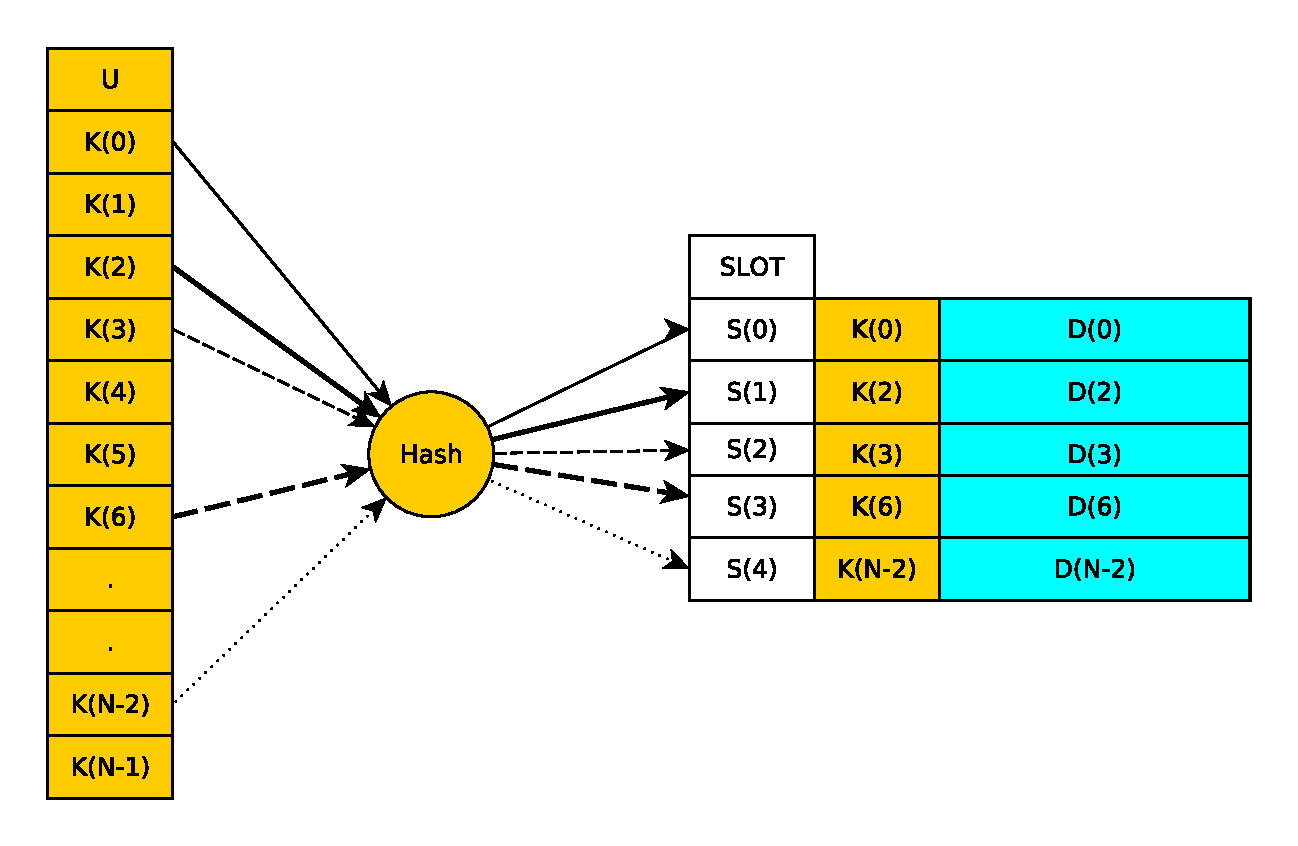
\includegraphics[scale=0.6]{fig/hash_table_example}	
	\caption{Princip fungov�n� ha�ovac�ch tabulek}
	\label{fig:hash_table_example}
\end{figure}
%%%%%%%%%%%%% HASH TABLE EXAMPLE %%%%%%%%%%%%%%%
 
Vzhledem k tomu, �e velikost tabulky je men��, ne� velikost univerza $|U|$,
budou nast�vat kolize. Kolize je p��pad kdy, dva r�zn� prvky univerza
$k_{1}, k_{2} \in U$ budou zobrazeny na stejn� slot : 
$f_{hash} (k_{1}) = f_{hash} (k_{2})$. S t�mto neduhem se d� vypo��dat mnoha 
zp�soby, jak uvid�me d�le v sekci \ref{sec:collisions}.

\section{Krit�ria kvality ha�ovac�ch funkc�}

Shr�me si nyn� z�kladn� krit�ria, kter� jsou d�le�i� pro ha�ovac� funkce.

\subsection{Uniformn� rozlo�en� v�stup�}

Pro dokonal� uniformn� rozlo�en� ha�ovac� funkce bychom pot�ebovali \textit{n�hodn�}
gener�tor a i kdybychom n�jak� m�li k dispozici, pak by sice dob�e dok�zal 
rozprost��t jednotliv� prvky do ha�ovac� tabulky, nicm�n� vzhledem k jeho n�hodn� 
povaze bychom je jen t�ko zp�t dohled�vali. Mus�me tedy zvolit jinou 
alternativu. Ha�ovac� funkce mus� b�t deterministick� a mus� dob�e aproximovat
uniformn� rozlo�en�. Uniformn� rozlo�en� v�stup� je p�edpokladem pro
n�zkou �asovou slo�itost ha�ovac�ch algoritm�, jak je vid�t z p��kladu
v sekci \ref{se:hash_function_design}.

\subsection{Odolnost proti koliz�m}

Uva�ujeme-li uniformn� rozlo�en� ha�ovac� funkce, pak dva kl��e u univerza
$U$ budou kolizn� (dle \textit{birthday attack}) asi po $2^{\frac{m}{2}}$ 
operac�ch vlo�en�\cite{NCHF_auto_design}. Pokud v�ak ha�ovac� funkce nebude
uniform� distribuovat v�sledky, pravd�podobnost kolize se rapidn� zv���.

\subsection{Lavinov� efekt}

Lavinov� efekt (angl. Avalanche effect) je vlastnost ha�ovac� funkce, p�i
kter� se rapidn� m�n� v�stup ha�ovac� funkce pro malou zm�nu vstupu. 
Funkce kter� maj� vysok� lavinov� efekt mohou odol�vat probl�mu shlukov�n�,
p�i kter�m se n�kter� ��sti univerza maj� tendenci shlukovat na v�stupu
do skupin.

\subsection{Rychlost}

Nesporn� v�hoda ha�ovac�ch tabulek je jejich rychlost. Dob�e navr�en� ha�ovac�
tabulka dosahuje za ur�it�ch okolnost� slo�itosti $\theta (1)$. Pokud je v�ak
v�po�etn� algoritmus p��li� slo�it�, m��e dan� funkce b�t pomal�. Je proto
nutn� db�t na to, �e p��li� pomal�, i kdy� dobr� algoritmus nemus� b�t
v�dy ten nejlep��. 

\section{N�vrh ha�ovac� funkce}
\label{se:hash_function_design}

V praxi je �asto sly�et n�zor, �e ha�ovac� funkce pracuj� v konstantn�m �ase.
To v�ak nen� pravda, nebo� v�kon ha�ovac� funkce z�le�� jednak na faktoru
zat��en� ha�ovac� tabulky a uniformnosti, s jakou dok�e ha�ovac� funkce
p���azovat kl��e do slot�.

Zam��me se nejprve na zat��en� tabulky a uva�me n�jakou podmno�inu univerza
v�ech kl��� $K \in U$, ha�ovac� tabulku $T$ s $m$ sloty a ozna�me $n = |K|$.
Pokud $n$ bude men�� ne� $m$, pak ha�ovac� tabulka bude skute�n� pracovat v 
$\theta (1)$, za p�edpokladu uniformn�ho rozlo�en� ha�ovac� funkce. Pokud ale
bude $m$ men�� ne� $n$, faktor zat��en� bude v�t�� ne� jedna a ha�ovac� tabulka
v konstantn�m �ase pracovat nebude. Uva�me $m=4$ a $n=5$. Pak za p�edpokladu
uniformn�ho rozlo�en� ha�ovac� funkce, s vlo�en�m p�t�ho prvku bude ha�ovac� 
tabulka pln� a n�m nezbude ne� vkl�dan� prvek za�adit na za��tek jednosm�rn�
v�zan�ho seznamu.

Existuje mnoho metod pro konstrukci ha�ovac� funkce, jako jsou nap��klad
\textit{metoda n�soben�}, \textit{metoda d�len�} a dal�� komplikovan�j��
p��stupy. V sou�asn� dob� existuj� velmi dobr� implementace obecn�ch ha�ovac�ch funkc�.
Av�ak ��dn� ha�ovac� funkce nem��e pracovat pro v�echna mo�n� univerza stejn�
dob�e. Jako p��klad uva�ujme ha�ovac� funkci navr�enou metodou d�len� :
$$ f_{hash}(k) = k \text{ mod } 8 $$ 
a d�le uva�ujme univerzum $U = \mathbb{N}$ a jeho
podmno�inu $K = \{1,2,3,4,8,13,22,71\}$, kterou budeme vkl�dat do tabulky.
Ha�ovac� funkce je schopna ulo�it $8$ ruzn�ch hodnot a v p��pad� 
na�eho v�b�ru mno�iny $K$, se n�m poda�� ulo�it v�echny, ani� by do�lo ke kolizi.
Co by se ale stalo, pokud bychom byli omezen� na univerzum pouze t�ch
p�irozen�ch �isel, kter� jsou d�liteln� osmi $U = \{x \in \mathbb{N}
\land x \text{ mod } 8 = 0\}$? Nemohli bychom vybrat ��dnou podmno�inu 
$F \in U$ takovou, kterou by funkce $f_{hash}$ nezobrazila pouze na jeden
slot.

Je vid�t, �e pokud m�me informace o univerzu mo�n�ch kl���, m��eme navrhnout
ha�ovac� funkci 'na m�ru' tak, aby m�la lep�� vlastnosti, ne� obecn�
ha�ovac� funkce. Tento �kol je v�ak obt��n� a neexistuj pro n�j obecn�
n�vod jak toho doc�lit. Mus�me se spolehnout na zku�enosti, znalosti a v 
neposledn� �ad� tak� na intuici. Nebo m��eme zvolit �pln� jin� p��stup
jak napov�d� kapitola \ref{sec:evolution_design}.

\subsection{Merkle-Damg\r{a}rdovo konstruk�n� sch�ma}
V oblasti kryptografick�ch ha�ovac�ch funkc� se Merkle-Damg\r{a}rdovo sch�ma \cite{merkle0} jedn�m ze z�kladn�ch
stavebn�ch kamen� modern�ch kryptografick�ch ha�ovac�ch funkc�.
Dokazuj� to nes�etn� implementace state of the art ha�ovac�ch funkc� na n�m zalo�en�. Jako
p�klad m��eme uv�st algoritmy \textit{MD5} \cite{rfc1321}, \textit{SHA-1} \cite{rfc3174},
\textit{SHA-2} \cite{rfc4634} nebo \textit{Tiger} \cite{tiger}.

Jedn� se o obecn� sch�ma pro v�stavbu ha�ovac�ch funkc� odoln�ch proti koliz�m z jednosm�rn�
kompresn� funkce. Sch�ma se skl�d� z $n$ blok� pevn� d�lky reprezentuj�c� vstupn� zpr�vu.
K nim koresponduj� jednosm�rn� kompresn� funkce. Ka�d� kompresn� funkce m� na vstupu blok vstupn�ch dat,
v�stup p�edchoz� kompresn� funkce a produkuje v�stup. Velikosti obou vstupu a v�stupu jsou toto�n�,
proto naz�v�me funkce kompresn�. Posledn� �l�nek v �et�zu kompresn�ch funkc� p�edstavuje vhodn� 
zarovn�n�. N�kdy se tak� pou��v� volitelna finaliza�n� komponenta. Sch�ma bl��e ilustruje obr�zek 
\ref{fig:merkle_damgard}.

Bylo nez�visle uk�z�no, �e pokud je pou�it� vhodn� 'vata'
(angl. \textit{padding}) pro zarovn�n� na spr�vnou velikost a kompresn� funkce jsou odoln�
proti koliz�m, pak vzniknuv�� ha�ovac� funkce je tak� odoln� proti koliz�m \cite{damgard0}.

D�vodem, pro� se zde zab�v�me kryptografick�m sch�matem je, �e jej pou��vaj� i mnoh� nekryptografick�
ha�ovac� funkce. I p�es to, �e tyto funkce nejsou kryptograficky bezpe�n� (co� ani nen� ��elem zaveden�
Merkle-Damg\r{a}rdova sh�matu), pou�it� kryptografick�ho sch�matu dod� do ha�ovac� funkce dodate�nou 
n�hodnost. Pou�it�m sch�matu doc�l�me v evolu�n�m algoritmu zna�n�ho zmen�en� prohled�van�ho prostoru
a tedy lep�� a rychlej�� konvergence algoritmu viz. d�le kapitola \ref{sec:evolution_design}.

Krom� Merkle-Damg\r{a}rdova sch�mata, exituj� i jin� konstruk�n� sch�mata, nap��klad Merkleho strom 
\cite{merkle1}, �asto pou��van� v \textit{P2P} s�t�ch,
struktura \textit{HAIFA} \cite{haifa} pou�it� v rodin� kryptografick�ch ha�ovac�ch funkc� \textit{BLAKE}
nebo funkce \textit{Sponge} \cite{sponge}. T�mito se zde v�ak zab�vat nebudeme.

 
\begin{figure}
	\centering
	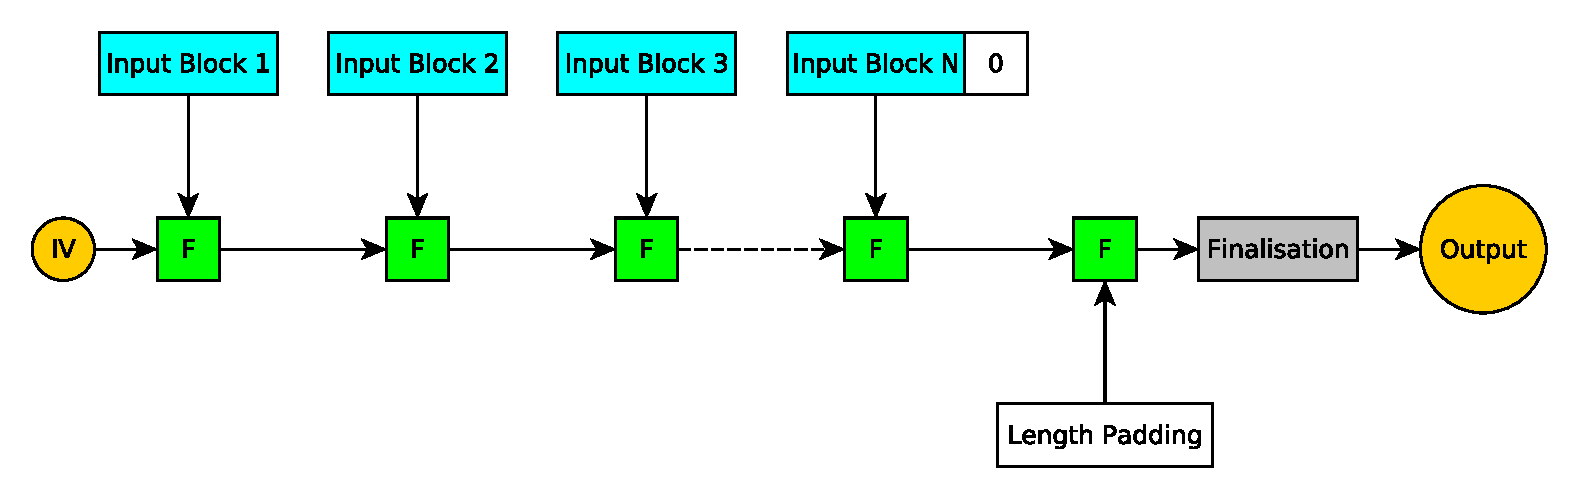
\includegraphics[width=\textwidth]{fig/merkle_damgard}
	\caption{Obecn� Merkle-Damg\r{a}rdovo sch�ma pro $n$ blok�.}
	\label{fig:merkle_damgard}
\end{figure}

\section{�e�en� koliz� p�i ha�ov�n�}
\label{sec:collisions}

Situaci, kdy ha�ovac� funkce zobraz� dva r�zn� kl��e na tent�� slot:
$f_{hash} (k_{1}) = f_{hash} (k_{2})$ naz�v�me ha�ovac� kolize nebo jen kolize. 
Kolize jsou ne��douc�m d�sledkem pou�it� ha�ovac�ch funkc�
a chceme se jim pokud mo�no vyhnout, nebo� z�sadn�m zp�soben negativn� ovliv�uj� 
�asovou slo�itost asociativn�ch pol�, kter� jsou na ha�ovac�ch funkc�ch postaven�. 
Pro dobr� pochopen� koliz� je nezbytn� uv�st m�ru zapln�n� ha�ovac� tabulky
neboli takzvan� faktor zat��en� $\alpha$ definovan� vztahem $\alpha = \frac{n}{m}$.
Pr�v� �asov� slo�itost tabulky z�le�� za p�edpokladu uniformn�ho rozlo�en� 
ha�ovac� funkce pr�v� na \textit{faktoru zat��en�}. 

Pou�it�m kvalitn� ha�ovac� funkce m��eme riziko koliz� do jist� m�ry minimalizovat, ale
s nar�staj�c�m faktorem zat��en� $\alpha$ roste i riziko kolize, kter� dos�hne 
ur�itosti p�i $\alpha = 1$, tedy v ha�ovac� tabulce nen� ji� ��dn� voln� slot.
V takov�m p��pad� mus�me kolizi vhodn�m zp�sobem �e�it. Zp�sob� jak takovou sitaci
�e�it je mnoho. My si v t�to sekci uvedeme ty, kter� jsou pro na�i pr�ci podstatn�.

\subsection{Z�et�zen� ha�ov�n�}

\begin{figure}
	\centering
	\begin{subfigure}[b]{0.49\textwidth}
		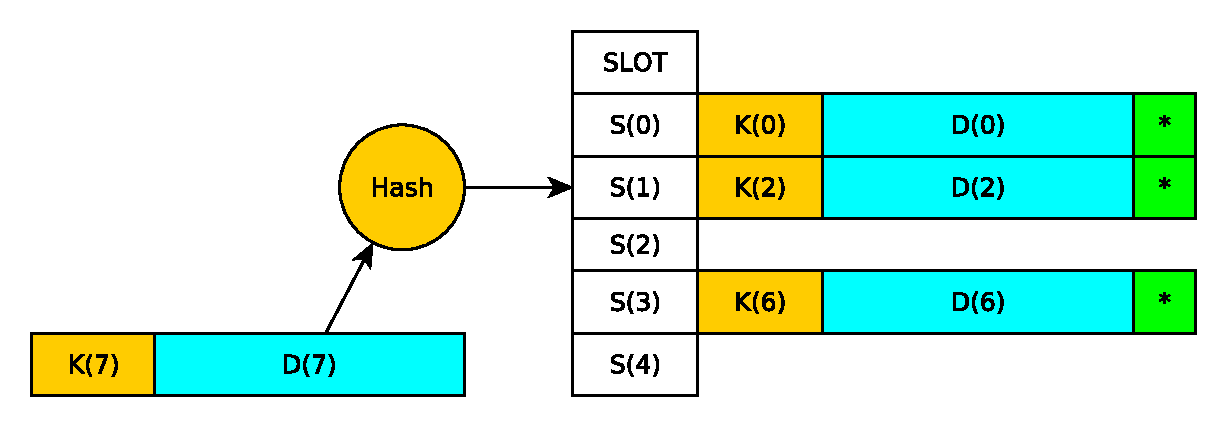
\includegraphics[width=\textwidth]{fig/chained_hashing_insert}
		\caption{Operace vlo�en� nov�ho prvku do ha�ovac� tabulky zp�sob� kolizi kl���.}
	\end{subfigure}
	\begin{subfigure}[b]{0.49\textwidth}
		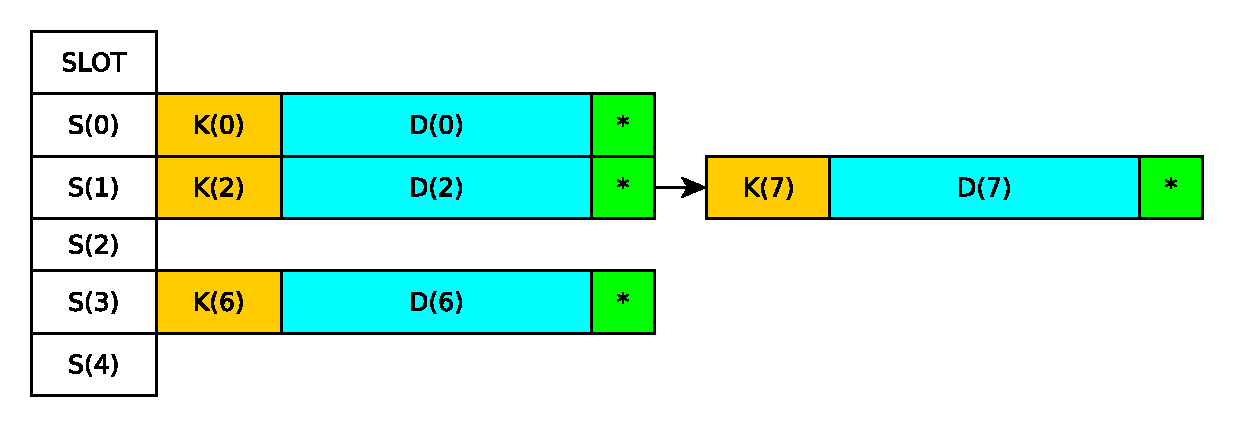
\includegraphics[width=\textwidth]{fig/chained_hashing_insert_result}
		\caption{Kolidovan� data se z�et�z� v jednosm�rn� v�zan�m seznamu.}
	\end{subfigure}
	\caption{Demonstrace �e�en� kolize za pou�it� v�zan�ho seznamu.}
	\label{chained_hashing}
\end{figure}

Nejjednodu��� a nejzn�m�j�� formou �e�en� koliz� je �et�zen� dat v dan�m slotu. Jednotliv� 
sloty jsou reprezentov�ny jednosm�rn� v�zan�m seznamem, jeho� polo�ky tvo�� data dohromady
s kl��em. �asov� slo�iost takov� implementace je:
\begin{itemize}
	\item v nejhor��m p��pad� $\theta (n)$, kdy v�echny prvky budou namapov�ny
	na jeden slot,
	\item v pr�m�ru bude $\theta (1 + \alpha)$, za p�edpokladu
	uniformn�ho rozlo�en�, kdy pravd�podobnost namapov�n� libovoln�ho
	prvku na konkr�tn� slot je $\frac{1}{m}$.
\end{itemize}

�asovou slo�itost lze vylep�it vhodnou heuristikou, jakou m��e b�t nap��klad sledov�n�
�etnosti vyhled�v�n� dan�ch kl��� s n�sledn�m vhodn�m p�euspo��d�n�m jednosm�rn� v�zan�ho
seznamu. Prostorov� slo�itost t�to implementace tak� nar�st�, nebo� sou��st� ka�d� polo�ky jednosm�rn�
v�zan�ho seznamu \textit{ll} je i ukazatel na dal�� prvek pot�ebn� pro z�sk�n�
dal��ho prvku seznamu \textit{next(ll)}. �e�en� koliz� z�et�zen�m kolidovan�ch 
polo�ek do jednosm�rn� v�zan�ho seznamu poskytuje za p�edpokladu uniformn�ho rozlo�en� dobr�
v�sledky a je v�razn� rychlej�� ne� samotn� jednosm�rn� v�zan� seznam. Existuj� v�ak i jin�
p��stupy, nab�zej�c� lep�� vlastnosti.

\subsection{Kuka��� ha�ov�n�}

Kuka��� ha�ov�n� je modern� p��stup k �e�en� ha�ovac�ch koliz�, za pou�it� dvou a v�ce ha�ovac�ch
funkci a jedn� nebo v�ce tabulek \cite{Cuckoo_hashing}. �ast� implementace zahruje pouze jednu
tabulku, v n�� m� ka�d� ha�ovac� funkce vyhrazena vlastn� prostor. Uva�ujme univerzum kl��� $U$
a velikosti ha�ovac� tabulky $m$. Pak na p��klad pro dv� ha�ovac� funkce 
$h_1, h_2$, kde $h_1 : U \rightarrow \{0,\ldots,r_1-1\}$ a $h_2 : U \leftarrow \{r_1,\ldots,r_2-1\}$ mus� platit
$|\{0,\ldots,r_1-1\} \cup \{r_1,\ldots,r_2-1\}| = m$ a celkov� po�et slot� ha�ovac� tabulky je $m$.

Opakem je implementace, kdy ka�d� ka�d� ha�ovac� fukce obsluhuje dedikovanou tabulku. Zde pro
jin� dv� funkce $h_3, h_4$ tvaru $h_3 : U \rightarrow \{0,\ldots,r_1-1\}$ a $h_4 : U \leftarrow \{0,\ldots,r_1-1\}$
mus� op�t platit $|\{0,\ldots,r_1-1\} \cup \{0,\ldots,r_1-1\}| = m$. Tedy �e ha�ovac� funkce mus� dokonale pokr�t
celou ha�ovac� tabulku.

N�zev Kuka��� ha�ov�n� je odvozen z chov�n� n�kter�ch druh� kuka�ek, kdy kuka�ky vytla�uj� vejce nebo sv� mlad�
z hn�zda. Toto chov�n� je velmi podobn� operaci vkl�d�n�. I p�es to, �e se rozhran� operace $Insert(S,x)$ nem�n� 
, v�razn� se m�n� jej� vnit�n� implementace. Operace vlo�en� prvku do tabulky, vybere jednu z dostupn�ch ha�ovac�ch
funkc� a pokus� se vlo�it prvek na p��slu�n� m�sto. Dojde-li ke kolizi, p�vodn� prvek je vytla�en a nahrazen prvkem nov�m.
Vytla�en� prvek je znovu vlo�en do tabulky, av�ak za pou�it� jin� ha�ovac� funkce. Tento postup se opakuje tak dlouho, dokud
doch�z� p�i vkl�d�n� ke koliz�m. Z�ejm� t�mto zp�sobem m��e doch�zet k cykl�m. Maxim�ln� po�et po sob� jdouc�ch vlo�en� je tedy
omezen konstantou. Cel� proces bl��e demonstruje algoritmus \ref{alg:cuckoo_hashing} a obr�zek \ref{fig:cuckoo_hashing}.

\begin{figure}
	\centering
	\begin{subfigure}[b]{0.53\textwidth}
		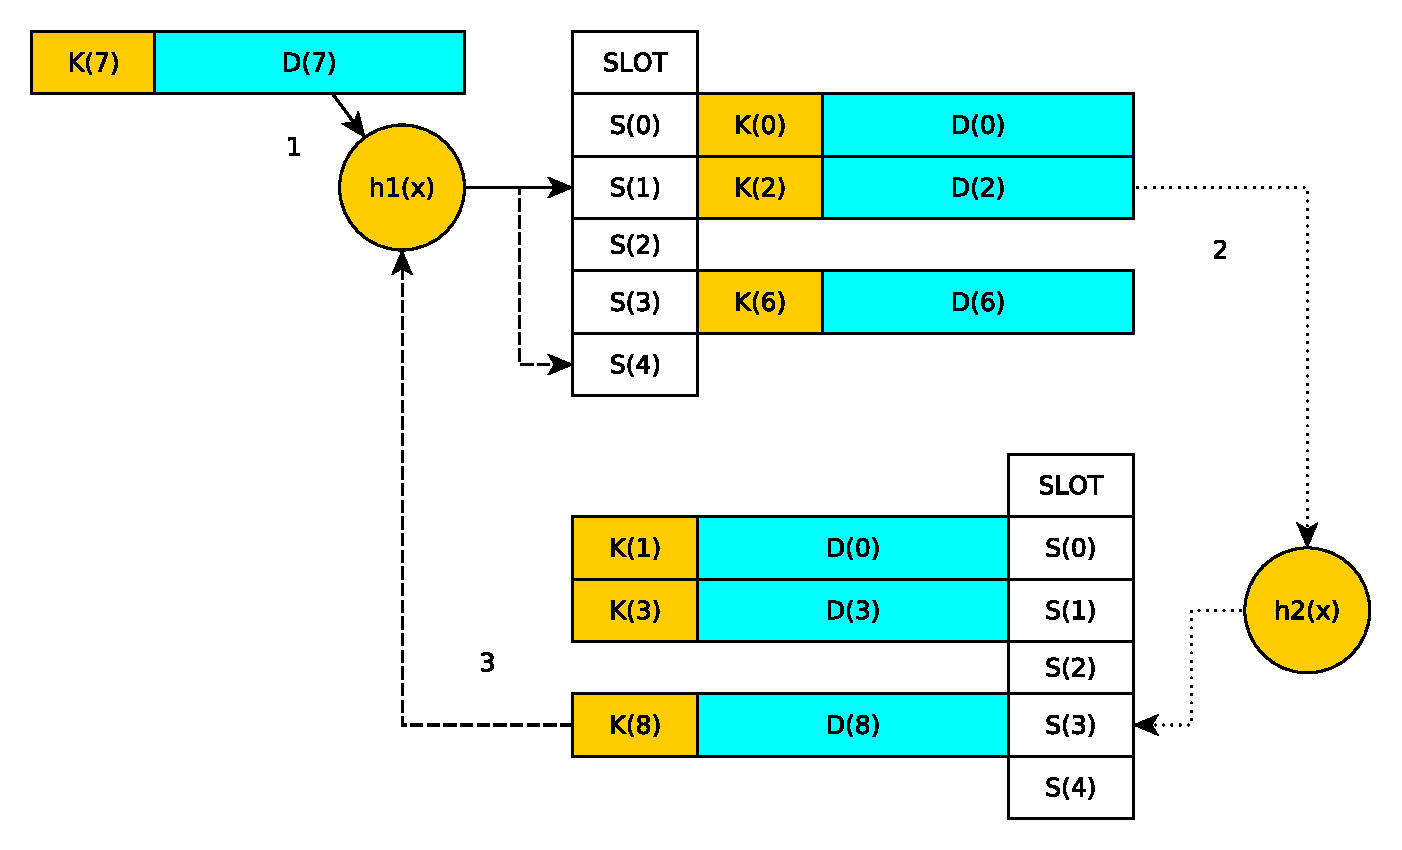
\includegraphics[width=\textwidth]{fig/cuckoo_hashing_insert}
		\caption{Kolize je �e�ena za pou�it� druh� ha�ovac� funkce.}
	\end{subfigure}
	\begin{subfigure}[b]{0.46\textwidth}
		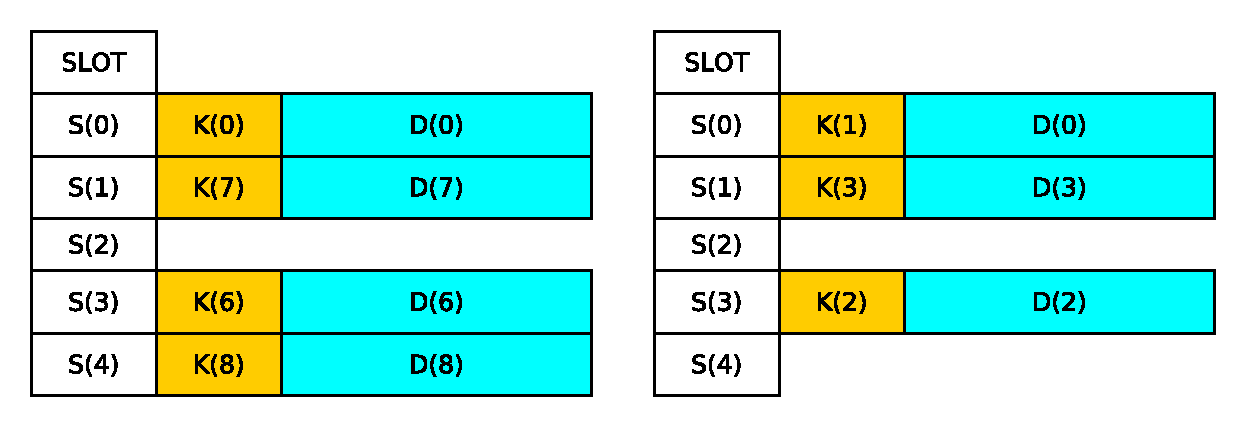
\includegraphics[width=\textwidth]{fig/cuckoo_hashing_insert_result}
		\caption{Data v tabulkce se po n�kolikan�sobn�m vytla�en� ust�l�.}
	\end{subfigure}
	\caption{Demostrace �e�en� kolize za pou�it� kuka���ho ha�ov�n�.}
	\label{fig:cuckoo_hashing}
\end{figure}

Pokud v pr�b�hu operace dosa�eno mezn� hodnoty $MaxLoop$, p�edpokl�d�me �e jsme narazili na cyklus. V takov�m p��pad� 
provedeme nejprve operaci \Call{rehash}{} a pot� zkus�me prvek vlo�it op�tovn�m zavol�n�m funkce \Call{insert}{x}.
Funkce \Call{rehash}{} zaji��uje, aby p�i op�tovn�m vlo�en� prvku do tabulky znovu nevzniknul cyklus. Toho se d�
dos�hnout nap��klad pou�it�m jin�ch ha�ovac�ch funkci \cite{Cuckoo_hashing}. Nen� t�eba znovu vytv��et ha�ovac� tabulku,
posta�� ha�ovac� tabulku proj�t a na ka�d� prvek uplatnit nejprve operace \Call{delete}{x}, kter� jej z tabulky odstran� 
a n�sledn� jej znovu vlo�it za pou�it� operace \Call{insert}{x}.

\begin{algorithm}
\begin{algorithmic}
\Function{insert}{x}
	\Repeat
		\State $x \leftrightarrow T_1[h_1(x)]$
		\If {$x = \bot$} \Return \EndIf
		\State $x \leftrightarrow T_2[h_2(x)]$
		\If {$x = \bot$} \Return \EndIf
	\Until{$!MaxLoop$}
	\State \Call{rehash}{}; \Call{insert}{x}
\EndFunction
\end{algorithmic}
\caption{Pseudok�d popisuj�c� operaci $insert$ za pou�it� kuka���ho ha�ov�n�.}
\label{alg:cuckoo_hashing}
\end{algorithm}

�asov� slo�itost v�hled�v�n� v tabulce za pou�it� Kuka���ho ha�ov�n� je v pr�m�ru $\theta(1)$. Pro n�s je ale
d�le�it�j��, �e �asov� slo�itost v nejhor��m p��pad� zust�v� tak� konstantn�. Je v�ak d�le�it� zohlednit 
n�sleduj�c� faktory:
\begin{itemize}
	\item Je nutn� pou��t takov� ha�ovac� funkce, kter� dob�e uniform� distribuuj� svoje v�stupy. Pokud by tento
	p�edpoklad nebyl spln�n, m��e b�t (a pravd�podobn� bude) �asto vol�na n�kladn� operace \Call{REHASH}{}.

	\item Operace \Call{REHASH}{} nezv�t�uje ani nezmen�uje kapacitu ha�ovac� tabulky. Vzhledem k tomu, �e ka�d� slot
	ha�ovac� tabulky pojme pr�v� jeden kl��, maxim�ln� faktor zat��en� $\alpha$ je pr�v� roven jedn� (co� je p�esn�
	opak chov�n� z�et�zen�ho ha�ov�n�, kdy za pou�it� v�zan�ho seznamu snadno dos�hneme $\alpha \geq 1$).

	\item Je dobr� po��tat s t�m, �e i za pou�it� v�ce ha�ovac�ch funkc� se koeficientu $\alpha = 1$ p�ibl���me jen
	vzd�len�. Op�tovn� pokusy o vlo�en� prvku do tabulky, kter� m� ji� koeficient $\alpha \approx 1$ nevyhnuteln�
	vy�st� ve vol�n� funkce \Call{REHASH}{}. Je tedy vhodn� podrobit Kuka��� ha�ov�n� n�jak� form� heuristiky, kdy
	bude jej� kapacita ve vhodn� okam�ik zv�t�ena, aby nedoch�zelo k opakovan�mu vol�n� funkce \Call{REHASH}{}.
\end{itemize}

\section{Anal�za existuj�c�ch �e�en�}
C�lem t�to sekce je podat p�ehled o existuj�c�ch state of the art obecn�ch ha�ovac�ch funkc�ch, proto�e n�kter�mi z t�chto
funkc� budeme porovn�vat n�mi navr�en� ha�ovac� funkce. Tak� budeme analyzovat, z jak�ch element�rn�ch operac� se 
dan� ha�ovac� funkce skl�daj�, co� n�m poslou�� p�edev��m pro n�vrh mno�iny funkc� d�le viz. kapitola  
\ref{sec:solution_design}. Nejprve se zam���me na kr�tk� popis vybran�ch ha�ovac�ch funkc� a pot� na samotn� rozbor.

\begin{itemize}
	\item \textit{MurmurHash2} \cite{murmurhash2} je druhou funkc� z rodiny ha�ovac�ch funkc� \textit{Murmur} vytvo�enou
		Austinem Appleby v roce 2008. Tato funkce se t�� velk� oblib� mezi ha�ovac�mi experty. V pr�b�hu let se v�ak 
		uk�zalo, �e trp� z�va�nou bezpe�nostn� chybou zahlcen� ha�ovac� funkce (angl. \textit{Hash-Flooding}), kdy spr�vnou
		volbou ha�ovan�ch kl��� dojde ke klastrov�n� v�stup� na jeden slot. Tato chyba m� za n�sledek extr�mn� zpomalen� 
		ha�ovac� tabulky vystav�n� nad touto funkc� a odep�en� slu�by (angl. Denial-of-Service) cel� aplikace. 
		
		Tato ha�ovac� funkce je pou�ita v mnoh�ch \textit{open-source} projektech, mezi n� pat�� i Apache Hadoop. 
		
	\item \textit{MurmurHash3} \cite{murmurhash3} je ji� t�et�m pokra�ovatelem funkc� z rodiny \textit{Murmur}. Dle
		autora se v nov� generaci jedn� o rychlej�� a robustn�j�� funkci. Je postavena na stejn�m z�kladu a nese si 
		s sebou jednoduchost a dobr� v�kon stejn� jako p�edchoz� verze. Bohu�el st�le trp� v��e zm�n�nou bezpe�nostn�
		chybou.
	
	\item \textit{CityHash} \cite{cityhash_slides}
	\item \textit{FarmHash} \cite{farmhash}
	\item \textit{lookup3} []
	\item \textit{SuperFastHash} []
	\item \textit{SpookyHash} []
\end{itemize}

Zam��me se nyn� na to, kter� element�rn� operace jsou vyu��v�n� v t�chto ha�ovac�ch funkc�ch. Tato informace n�m pom��e se
zorientovat v problematice n�vrhu a umo�n� n�m dob�e zvolit funkce i termin�ly v n�mi navr�en�ch ha�ovac�ch funkc�. N�kter�
ha�ovac� funkce pracuj� nejen s element�rn�mi ha�ovac�mi funkcemi, ale i s jejich vysoko�rovnov�mi kombinacemi. Tyto
takzvan� \textit{mixovac� komponenty} nebudeme ch�pat jako samostatn� operace, ale rozlo��me je v na�� anal�ze na
element�rn� operace. Pro lep�� orientaci v problematice poslou�� p�ehledov� tabulka \ref{tab:generic_hashes_analysis}.
Rozbor byl prov�d�n z referen�n�ch implementac�, kter� jsou v�echny krom� funkce \textit{FarmHash} obsa�eny v bal�ku
\textit{SMHasher} []. Ofici�ln� referen�n� implementace funkce \textit{FarmHash} je mo�n� z�skat z repozit��e na
str�nce \textit{Github} \footnote{https://github.com/google/farmhash/blob/master/src/farmhash.cc}. Implementace ha�ovac�ch
funkc� obsahuj� opravdu �irok� spektrum oper�tor�. N�s budou zaj�mat pouze ty, kter� jsou pou�ity pro samotnou tvorbu
v�stupu. Nesm� n�s tedy zm�st nap��klad pou�it� logick�ho sou�tu nebo sou�inu v �id�c�ch konstrukc�ch nebo operace
s��t�n� a od��t�n� pou��t� pro krokov�n� vstupu po bloc�ch ur�it� velikosti. 

Ve zdrojov�ch k�dech referen�n�ch implementac� jednotliv�ch ha�ovac�ch funkc� m��eme vid�t n�kter� opakuj�c� se vzory.
V�dy je pou�ita jedna nebo v�ce aritmetick�ch operac�. V na�em v�b�ru se v�dy jedn� o s��t�n� ($+$) , n�soben�  ($*$) nebo
jejich spole�nou kombinaci. Dal�� ned�lnou sou��st� dobr� ha�ovac� funkce je volba posunu nebo rotace. V�t��na vybran�ch
funkc� spol�h� na rotace, men�ina pot� na posuny. Najdou se i takov� implementace, kter� pou��vaj� ob� dv�, ale za
prim�rn� operaci lze pova�ovat jen rotaci. Posuny jsou v takov�m p��pad� pou�ity jako sou��st vysoko�rov�ov� 
\textit{mixovac� komponenty}.

\begin{table}[!ht]
	\centering
	\begin{tabular}{lccccccccccc}
		\hline
		Operace            & $*$ & $/$ & $+$ & $-$ & Posuny & Rotace & AND & OR & XOR & $\neg$ & Konstanty \\
		\hline
		MurmurHash2   & \checkmark & & & & \checkmark & & & & \checkmark & & \checkmark \\
		MurmurHash3   & \checkmark & & \checkmark & &  & \checkmark & & & \checkmark & & \checkmark \\
		lookup3              & & & \checkmark & \checkmark & & \checkmark & & & \checkmark & & \checkmark \\
		FarmHash         & \checkmark & & \checkmark & & \checkmark & \checkmark & \checkmark & & \checkmark & & \checkmark  \\
		CityHash          & \checkmark & & \checkmark & & \checkmark & \checkmark & & & \checkmark & & \checkmark \\
		SpookyHash     & & & \checkmark & & & \checkmark & & & \checkmark & & \\
		SuperFastHash & & & \checkmark & & \checkmark & & & & \checkmark & & \\
		\hline		
	\end{tabular}
	\label{tab:generic_hashes_analysis}
	\caption{Anal�za existuj�c�ch ha�ovac�ch funkc� z pohledu pou�it�ch elementarn�ch operac�.}
\end{table}

Dal�� skupinu �asto pou��van�ch operac� tvo�� operace logick� a bitov�. Zde v drtiv� v�t��n� naraz�me na operaci XOR. Z��dka
pou��vanou operac� je logick� sou�in (AND). Naopak nikdy nejsou pou�ity operace logick�ho sou�tu (OR) a jedni�kov�ho
dopl�ku ($\neg$). Posledn� skupninou jsou konstanty. Ty jsou pou�ity pro p�iveden� dodate�n� n�hodnosti do ha�ovac� funkce.
�asto se jedn� o prvo��sla, kter� sv�mi specifick�mi vlastnostmi netrp� na shlukov�n� v�stupu. Setk�me se v�ak i s jin�mi 
konstantami, jako nap��klad konstanta \texttt{0xdeadbeef} pou�it� v p��pad� funkce \textit{lookup3}.

\chapter{Evolu�n� n�vrh}
\label{sec:evolution_design}

% Chapter INTRO
Evolu�n� n�vrh je netradi�n� discipl�na, kter� vyu��v� evolu�n� algoritmy
k n�vrhu. Evolu�n� algoritmy spadaj� do oblasti um�l� 
inteligence. Specifickou vlastnost� mnoha �loh spadaj�c�ch do obasti um�l� 
inteligence je, �e �asto vhodn�m zp�sobem prohled�vaj� prostor $U$,
reprezentuj�c� v�echna mo�n� �e�en� (kandid�tn�) dan� �lohy 
\cite{evolution_hardware}. Evolu�n� algoritmy se daj� pova�ovat za speci�ln� metodou 
prohled�v�n� prostoru kandid�tn�ch �e�en�.

% Section Natural computing
\section{Po��t�n� podle p��rody}
\label{sec:natural_computing}
Po��t�n� podle p��rody (Natural computing) je sohrn� term�n pro tvorbu 
inteligentn�ch stroj� napodobov�n�m biologick�ch proces�, chov�n� �iv�ch 
tvor� nebo jejich mechanism�. �ad�me sem tak� v�po�etn� paradigmata, kter� 
svoji inspiraci nalezla v p��rodn�ch procesech nebo pou�it� organism� a 
jin�ch netradi�n�ch materi�l� jako v�po�etn�ch platforem. M�ra do jak� je 
p��rodn� fenom�n napodoben se r�zn�. Od T�m�� �pln�ho napodoben� a� po 
inspiraci. 

Jedn�m z motiv� pro vznik alternativn�ch v�po�etn�ch p��stup� a po��t�n� 
podle p��rody je lep�� splynut� s re�ln�m sv�tem a jeho prob�my.
V tomto kontextu je vhodn� zm�nit \textit{soft-computing}. \textit{Soft-computing}
je podmno�inou po��t�n� podle p��rody, b�vaj� sem za�azov�ny 
neuronov� s�t�, \textit{Support Vector Machines}, fuzzy syst�my, evolu�n� 
algoritmy a teorie chaosu. Postupy spadaj�c� do \textit{Soft-computing} 
toleruj� nep�esnosti a nejistotu ��m� dosahuj� vysok� robustnosti a 
lep��ho vztahu s realitou. Po��t�n� podle p��rody ve sv�j prosp�ch pou��v� 
procesy zejm�na fylogeneze, ontogeneze a epigeneze. Fylogeneze ozna�uje proces
evoluce druh�, ontogeneze proces v�voje mnohobun��n�ho organismu a epigeneze
je n�jak� proces, kter� nast�v� v ji� slo�it�j��m organismu 
(sem �ad�me nap��klad neuronov� s�t�).
D�le se se po��t�n� podle p��ody inspirovalo procesy vznikaj�c�mi ve spole�nosti, 
v usuzov�n� jedinc� apodobn�. My se zde budeme zab�vat hloub�ji pouze fylogenez�, nebo� 
pr�v� na n� je zalo�ena my�lenka evolu�n�ch algoritm�.

\section{Evolu�n� algoritmy}

Fylogeneze je proces evoluce druh�. Evoluce je umo�n�na schopnost� reprodukce jednotliv�ch
jedinc�, kdy potomkov� se od sv�ch rodu�� li�� jen velmi m�lo. P�i reprodukci v�ak doch�z� tak�
k n�hodn�m ob�asn�m mutac�m, kter� zabezpe�uj� dostate�nou diferzitu a vznik� tak nov�
genetick� materi�l. Na fylogenezi jsou zalo�en� evolu�n� algoritmy. 

Evolu�n� algoritmy lze ch�pat jako speci�ln� optimaliza�n� metodu nad prostorem 
$$U = D_{1} \times D_{2} \times D_{3} \times \ldots \times D_{n}$$
v�ech kandid�tn�ch �e�en�. Takov� prostor je pak kart�zsk� sou�in dom�n, kde
jednotliv� dom�ny univerza mohou nab�vat
hodnot z p�edem zn�m�ch, �asto n�jak omezen�ch interval� \cite{evolution_hardware}.  

V matematick� optimalizaci, bychom se sna�ili hledat hodnoty $x \in U$ takov�,
pro kter� je hodnota ��elov� funkce
$$ f : U \to \mathcal{R} $$
minim�ln� (hled�n� maxima lze �pravou ��elov� funkce p�ev�st na hled�n� minima).
Minima mohou b�t glob�ln� nebo lok�ln�, ostr� nebo neostr�. �e��me tedy �lohu,
kdy hled�me n�jak� argument, jeho� hodnota ��elov� funkce spad� do mno�iny optim�ln�ch
hodnot ��elov� funkce \cite{nlprog}.
$$ argmin_{x}\{f(x)|x \in U\} $$		
V kontextu evolu�n�ch algoritm� naz�v�me $f$ funkc� \textit{fitness} a nehled�me 
argument $x$, pro n�j� je funkce $f$ minim�ln�, ale posta�uje n�m naj�t argument $x$ 
takov�, �e $f(x)$ spln� n�jak� p�edem d�n� ukon�ovac� podm�nky.

\subsection{Princip}
Evolu�n� algoritmy jsou inspirovan� procesem reprodukce jedinc� nap��� generacemi.
Na za��tku v�po�tu algoritmu vytvo��me po��te�n� populaci $P_{0}$, tj.
populaci generace nula o p�edem zn�m� velikosti $n$.
Volba jedinc� do po��te�n� populace jsou r�zn�, m��eme nap��klad s�hnout po n�hodn�m 
v�b�ru nebo volit jedince za pou�it� vhodn� heuristiky.

%$$ \mathcal{P}_{0} = \{x|x \in U \land vyber\_do\_po��te�n�\_populace(x) \} $$

V ka�d�m dal��m kroku evolu�n�ho algoritmu, kter� naz�v�me generace, je nejprve vybr�no
$m$ vhodn�ch jedinc� z generace p�edchoz� $P_{t - 1}$, kte�� n�m tvo�� mno�inu rodi��. Aplikac�
genetick�ch oper�tor� nad mno�inou rodi�� vznikne mno�ina potomk�, N�sledn� se z obou
mno�in vybere nov� generace $P_{t}$ o velikosti $n$ a cel� process (zn�zorn�n na diagramu \ref{fig:eaflow})
se opakuje. Zp�soby v�b�ru rodi�u jsou r�zn� stejn�
tak jako mo�n� genetick� oper�tory. Ob�ma se budeme zab�vat pozd�ji.

%%%%%%%%%%%%% EVOLUTION ALGORITHM FLOWCHART %%%%%%%%%%%%%%%
\begin{figure}[!ht]
	\centering
	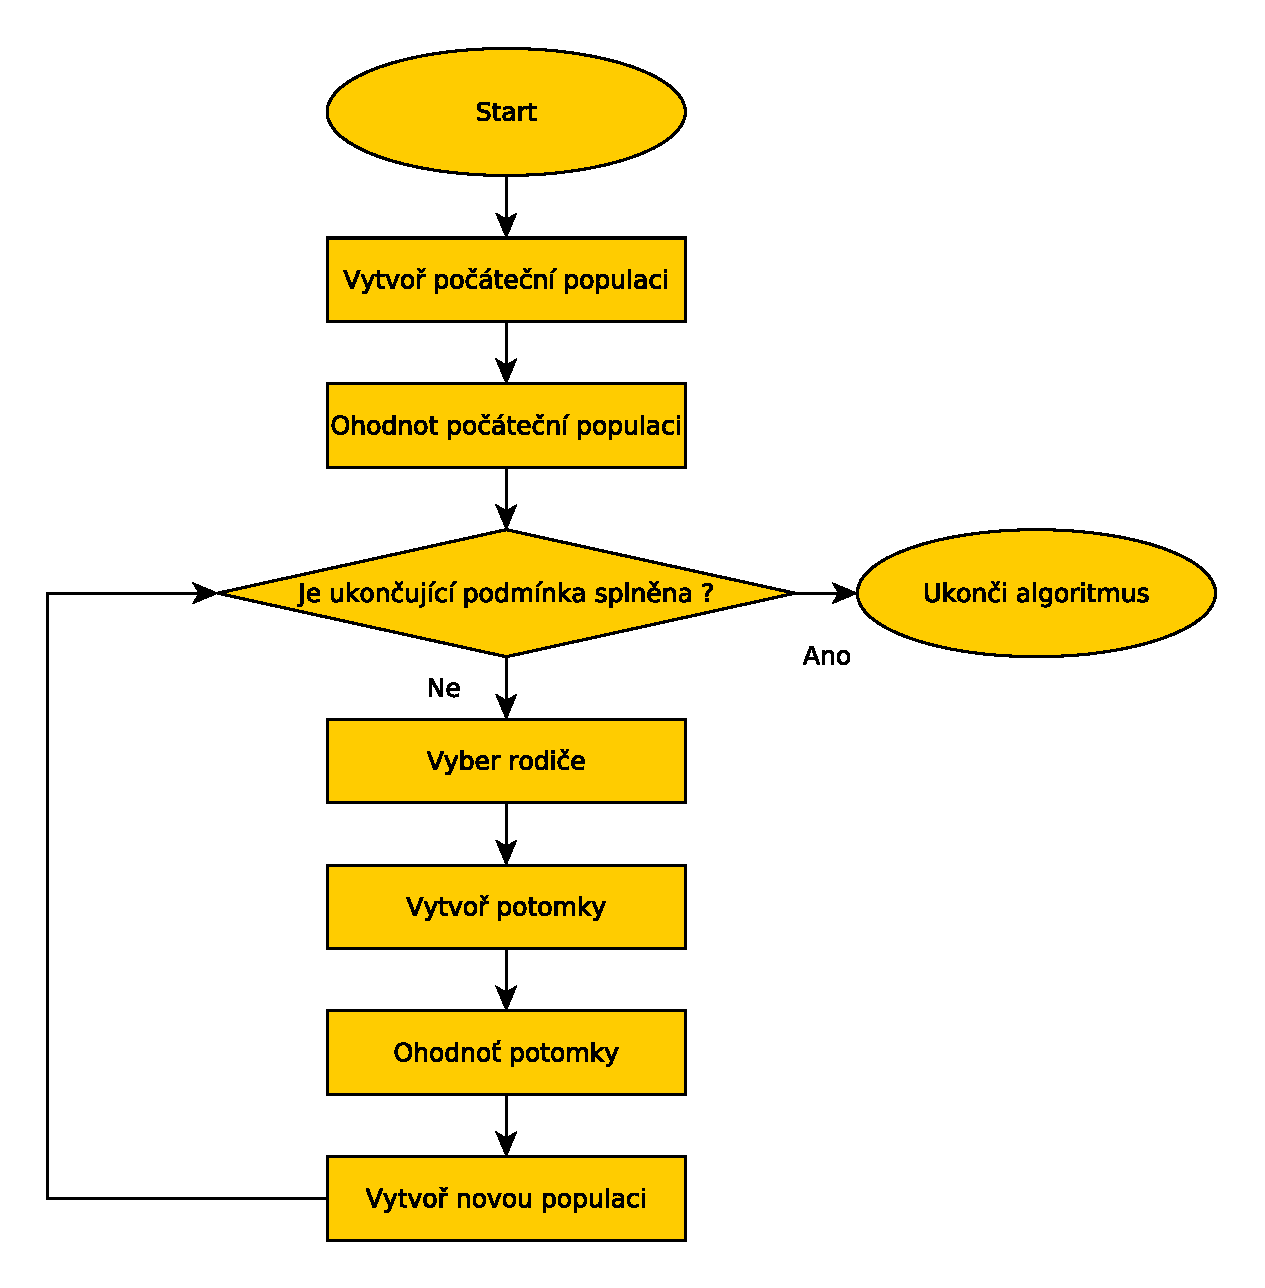
\includegraphics[scale=0.4]{fig/evolution_algorithm_flowchart}	
	\caption{Obecn� postup v�po�tu evolu�n�ho algoritmu}
	\label{fig:eaflow}
\end{figure}
%%%%%%%%%%%%% EVOLUTION ALGORITHM FLOWCHART %%%%%%%%%%%%%%%

\subsection{Fitness funkce}
Fitness funkce je obdoba ��elov� funkce z oboru matematick� optimalizace. N�zev fitness
poch�z� z oboru evolu�n� biologie, kde hodnota fitness popisuje biologickou zdatnost jedince
\cite{evolution_hardware}. Vstupem fitness funkce je (v jednodu���m p��pad�) jedinec
reprezentovan� chromozomem a v�stupem je hodnota reprezentuj�c� zdatnost jedince.

Ve slo�it�j��ch p��padech je nutn� rozli�ovat mezi prostorem genotyp� a fenotyp�. Genotypem
naz�v�me v kontextu evolu�n�ch algoritm� prostor v�ech mo�n�ch �e�en�, tedy 
v�ech mo�n�ch chromozom�. Fenotyp je soubor charakteristik, projev� a chov�n�,
jimi� se dan� jedinec reprezentovan� ur�it�m chromozomem projevuje.
Zobrazen� z prostoru genotyp� do prostoru fenotyp� lze potom vyj�d��t n�sledovn�:
$$ f_{phenotype} : U \to \mathcal{F}, $$
Potom je v�ak nutn� modifikovat na�i fitness funkci n�sledovn� :
$$ f : \mathcal{F} \to \mathcal{R} $$
a cel� proces evaluace jedince bude pot� kompizice t�chto dvou funkc� :
$$ f_{eval} = f \circ f_{phenotype}$$

Volba pota�mo n�vrh vhodn� fitness funkce je zna�n� obt��n�. Neexistuje ��dn� obecn�
p�edpis pro jejich n�vrh. Mus�me se spol�hat na obecn� pravidla, zku�enosti nebo 
intuici. Velk� mno�stv� dob�e zakomponovan�ch informac� o probl�mu ve fitness funkci je
dobr�m z�kladem pro �sp�n� evolu�n� algoritmus. Obecn� tedy plat�, �e 
vhodn� zvolen� fitness funkce m� zna�n� dopad na kvalitu v�sledn�ho �e�en�.

\subsection{Zp�soby selekce}
Zp�soby selekce jsou d�le�it�m faktorem p�i n�vrhu evolu�n�ho algoritmu. Selekce
je proces, p�i n�m� se vyb�raj� rodi�e z aktu�ln� populace ur�en� k reprodukci. 
Dobr� selek�n� algoritmus mus� b�t schopen up�ednost�ovat jedince s vysokou hodnotou
fitness funkce, na druhou stranu mus� zajistit dostate�n� mno�stv� genetick�ho 
materi�l� pro dal�i generace. �asto vyu��van� selek�n� mechanismy, zejm�na v kontextu
genetick�ch algoritm� jsou nap��klad \cite{selection_schemes_comparison} :

\begin{itemize}
	\item \textit{deterministick� selekce}, kde se do mno�iny rodi�� vybere $k$
		jedinc� z aktu�ln� populace s nejvy��� hodnotou fitness,
		
	\item \textit{proporcionln� selekce}, kde pravd�podobnost v�b�ru jedince $i$ je 
		rovna vztahu $p_{i} = \frac{f(i)}{\sum_{j=1}{N} f(j)}$,
		
	\item \textit{turnajov� selekce}, kdy je v n�kolika kolech turnaje postupn� 
		porovn�no n�kolik n�hodn� vybran�ch jedinc� a v�t�z turnaje je za�azen
		do mno�iny rodi��. Turnaj provedeme $n$-kr�t, kde $n$ je po�adovan� mohutnost
		mno�iny rodi��. 
\end{itemize}

\subsection{Genetick� oper�tory}
Evolu�n� algoritmy vyu��vaj� k���en� i mutaci, oba mechanismy jsou p�evzaty z
oboru bun��n� biologie, kde se uplat�uj� v procesu reduk�n�ho d�len� bun�k.

Oper�tor mutace se aplikuje na potomka
a vytvo�� z n�j potomka mutovan�ho. Stejn� jako v biologii, mutace se vyskytuje
pouze v mal�m po�tu p��pad�. Na�im c�lem je prozkoumat prostor $U$ postupn� a
konvergovat k dobr�m �e�en�m. V p��pad� vysok� pravd�podobnosti mutace se ji�
nejedn� o algorigmus \textbf{evolu�n�}, n�br� \textbf{revolu�n�} a algoritmus p�ipom�n� 
sp��e n�hodn� prohled�v�n�. Oper�tor mutace je velmi d�le�it�, nebo� zanesen�
n�hodne mutace zaji��uje nov� genetick� materi�l, ��m� je algoritmus jednou za
�as nucen prozkoumat vzd�len�j�� bod prostoru. Neuv�zne tak v lok�ln�ch extr�mech.

P�i k���en� doch�z� k p�enosu ��st� chromozom� rodi�� na potomka. Zp�sob� k���en�
existuje cel� �ada. Obecn� v�ak plat�, �e zp�sob k���en� je z�visl� na zvolen� 
reprezentaci. Pokud m�me jedince reprezentovan�ho grafem, oper�tor k���en� 
se bude zna�n� odli�ovat od p��padu, kdy m�me jedince reprezentovan�ho bin�rn�m
vektorem. 

Uve�m� si zde alespo� nejzn�m�j�� druhy k���en� nad bin�rn� reprezentaci, jimi� jsou:
\begin{itemize}
	\item \textit{jednobodov� k���en�}, kdy se ur�� m�sto k���en� ur�uj�c�,
		kter� ��st chromozomu doputuje do potomka.
		
	\item \textit{dvoubodov� k���en�} je obdobou v��e zm�n�n�ho, av�ak pro dva body
		k���en� a
	\item \textit{uniformn� k���en�}, kter� je do zna�n� m�ry zobecn�n�m v��e zm�n�n�ch.
		 Ur�� $n$ gen� v chromozomu, jejich� hodnoty jsou vyst��d�ny.
\end{itemize}

\subsection{N�vrh evolu�n�ho algoritmu}

Kvalita n�mi navr�en�ho evolu�n�ho algoritmu, je zejm�na z�visl� na n�sleduj�c�ch faktorech:
\begin{enumerate}
	\item reprezentace probl�m� a jeho k�dov�n�,
	\item pou�it� fitness funkce,
	\item zobrazen� z prostoru genotyp� do prostoru fenotyp�,
	\item volbou genetick�ch oper�tor� a zp�soby selekce,
	\item nastaven�m parametr� genetick�ho algoritmu.
\end{enumerate}

Prostor ka�d�ho probl�mu �e�iteln�ho evolu�n�my algoritmy je jin�. Neexistuje tedy obecn�
evolu�n� algoritmus, kter� by kvalitn� �e�il v�echny probl�my. Toto tvrzen� podporuje takzvan�
\textit{No Free Lunch} teor�m. Pokud uv��me dostate�n� velk� po�et optimaliza�n�ch probl�m�,
neexistuje ��dn� optimaliza�n� algoritmus, kter� projde ka�d� bod prostoru $U$ pr�v� jednou
a v pr�m�ru bude efektivn�j�� ne� ostatn� optimaliza�n� algoritmy \cite{nflteorem, evolution_hardware}. 
Z tohoto tvrzen� plyne, �e chceme-li �e�it optimaliza�n� probl�m skute�n� efektnivn�, mus�me 
do na�eho evolu�n�ho algoritmu \textbf{vlo�it co nejv�ce informac�} o probl�mu prost�ednictv�m 
zejm�na polo�ek zm�n�n�ch v��e.

\subsection{Genetick� algoritmy}

Evolu�n� algoritmy popisuj� mno�inu algoritm�, jejich� �innost je ur�ena procesem Darwinovsk�
evoluce. Na druh� stran� je v�ak neomezuje natolik, aby se od sebe nemohly (n�kdy i velmi
v�znamn�) li�it.

Asi nejv�znam�j��m ��stupcem evolu�n�ch algoritm� jsou genetick� algoritmy. Jedinci jedn� populace
jsou reprezentov�ny �et�zcem (chromozomem) bin�rn�ch, celo��seln�ch nebo i re�ln�ch hodnot.
Inici�ln� populace vznik� bu� n�hodn� nebo za pou�it� vhodn� heuristiky. Uplat�uj� se zde v�echny
b�n� selek�n� mechanismy a stejn� tak zde najdeme pou�ity v�echny druhy metod k���en�.
Mutace se takt� pou��v�. Nev�hodou mohou n�kdy b�t chromozom� pevn� d�lky.

\subsection{Evolu�n� strategie}

Dal��m zaj�mav�m algoritmem jsou evolu�n� strategie. Jejich nejv�t�� zaj�mavost� je, �e
se spol�haj� pouze na oper�tor mutace. K���en� se zde nevyskytuje. Nov� generace se zde
vytv��ej� zejm�na tak, �e rodi�ovsk� populace je mutov�na p�i�ten�m hodnoty norm�ln�ho rozlo�en� s nulovou
$x' = x + \mathcal{N}(0, \sigma)$
st�edn� hodnotou. Rozptyl $\sigma$ se m�n� na z�klad� toho, jak dob�e algoritmus aktu�ln�
konverguje. Jako selek�n� mechanismy se u��v� tot�ln� elitismus ve variant�ch $(\mu + \lambda)$
a $(\mu, \lambda)$ \cite{ES}. Uva�ujeme-li $\mu$ mno�inu rodi�� a $\lambda$ mno�inu jejich
potomk�, pak :

\begin{itemize}
	\item $(\mu + \lambda)$ vybere do dal�� generace nejlep�� jedince z mno�iny
		rodi�� a potomku
	\item $(\mu, \lambda)$ vybere do dal�� generace jen ty nejlep�� potomky. Rodi�ovsk�
		generace tedy vym�r�.
\end{itemize} 

\section{Genetick� programov�n�}

Pro na�� pr�ce je zejm�na zaj�mav� genetick� programov�n�, nebo� pr�v� to jsme zvolili 
jako evolu�n� algoritmus pro �e�en� na�eho probl�m�. Sezn�m�me se s n�m podrobn�ji a 
proto mu v�nujme celou sekci.

Genetick� programov�n� je speci�ln�m druhem evolu�n�ho algoritmu, kde jednotlivce a 
cel� populace tvo�� po��ta�ov� programy. V�po�et iterativn� transformuje po��ta�ov�
programy na jin� po��ta�ov� programy aplikac� genetick�ch oper�tor�, kter� jsou 
pro genetick� programov�n� specifick�. V�stupem genetick�ho algoritmu
je v p��pad�, �e usp�je, n�jak� program. 

\subsection{Reprezentace}
Evolvovan� programy mus�me vhodn� reprezentovat. Mus�me p�� tom kl�st d�raz na to,
�e programy je mezi sebou t�eba k���it, mutovat a obecn� na nich prov�d�t nutn�
genetick� operace. Na druh� stran� v�ak chceme volit takovou reprezentaci, kter�
n�m umo�n� programy evaluovat, tud�� vykon�vat je nad zadan�m vstupem. 

Jedinci v populaci jsou reprezentov�n� rad�ji jako \textit{abstraktn� syntaktick� stromy}
\cite{GPTutorial} ne� jako ��dky programu. Uk�zka jedince v genetic�m programov�n� je na
diagramu \ref{fig:exampletree1} a zobrazuje jedince reprezentovan�ho programem
\texttt{max(min(x,y), 5 + z)}. Stromy se skl�daj� z uzl� a list�. Listy jsou
reprezentov�ny termin�ln�m symbolem z mno�iny termin�l� $T$ a uzly jsou reprezentov�ny
funkc� z mno�iny $F$. Na diagramu \ref{fig:exampletree1} mno�inu funkc� tvo�� 
$F = \{max, min, +\}$ a mno�inu termin�lu $T = \{5, x, y, z\}$. Mno�iny povolen�ch
funkc� a termin�l� dohromady tvo�� primitivn� mno�inu syst�mu. Prostor mo�n�ch 
�e�en� m��eme tedy definovat jako mno�inu v�ech mo�n�ch strom�, kter� mohou vzniknout
kombinac� funkc� a termin�l� :

$$ U = \{t | t=(FT)^{n}, 0 \leq n \leq max\_depth \}$$

Programov� reprezentace strom� se li�� v z�vislosti na pou�it�m programovac�ho jazyku.
Plat� v�ak, �e 
v pros�ed�ch n�ro�n�ch na v�po�etn� v�kon je pam�ov� n�ro�nost grafov� reprezentace
neefektnivn�. Stromov� reprezentace lze u��t i nep��mo za pou�it� prefixov� notace.
P�� pou�it� prefixov� notace se z�vorky stanou nadbyte�n�mi a program lze v pam�ti
ulo�it jako \textit{line�rn� sekvenci symbol�}. Jako p��klad poslou�� diagram 
\ref{fig:exampletree1}, tedy \texttt{max min x y + 5 z}. Volba reprezentace tedy
v kone�n�m d�sledk� z�le�� na u�ivateli a jeho preferenc�ch, po�adavc�ch a prost�ed�. 

%%%%%%%%%%%%% TREE REPRESENTATION EXAMPLE 1 %%%%%%%%%%%%%%%
\begin{figure}[!ht]
	\centering
	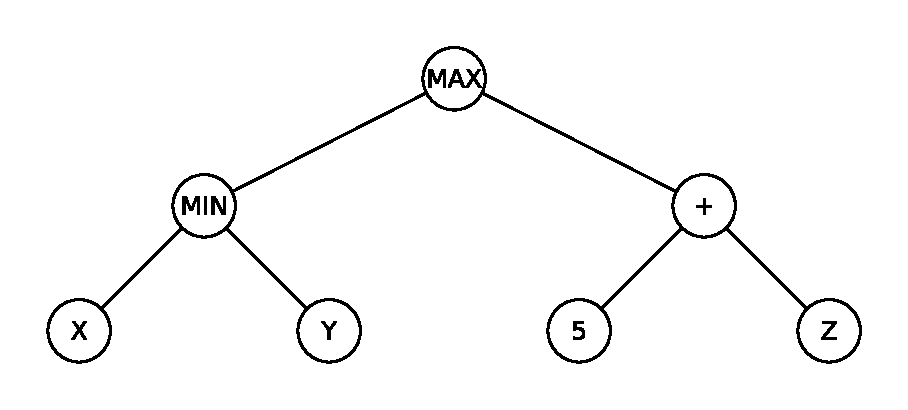
\includegraphics[scale=0.6]{fig/example_tree1}	
	\caption{Uk�zka reprezentace programu max(min(x,y), 5 + z)}
	\label{fig:exampletree1}
\end{figure}
%%%%%%%%%%%%% TREE REPRESENTATION EXAMPLE 1 %%%%%%%%%%%%%%%

\subsection{Inicializace nult� populace}

Pro inicializaci nult� populace plat� obecn� pravidla. M��eme ji bu� volit n�hodn�
nebo pou��t n�jakou vhodnou heuristiku. Je zde v�ak specifick� vlastnost, kterou 
mus�me vz�t do �vahy. Na�e programy nemaj� pevn� omezenou velikost (d�lka
chromozomu je prom�nn�). Jak velk� n�hodn� programy tedy generovat? Existuj� t�i
z�kladn� p��stupy:

\begin{enumerate}
	\item \textit{Full} metoda, kdy n�hodn� vygenerujeme strom do maxim�ln� povolen�
		hloubky,
	\item \textit{Grow} metoda, generujeme stromy prom�nliv� d�lky a tvaru (maxim�ln�
		hloubka je omezena) a
	\item \textit{Ramped half-and-half}, kdy polovina populace je generov�na metodou
		\textit{Grow} a druh� metodou \textit{Full}, za prom�nliv� maxim�ln� hloubky.
\end{enumerate}

Metoda Full v�dy a za v�ech okolnost� generuje pln� stromy. V uzlech jsou funkce
vyb�r�ny n�hodn� z mno��ny $F$ a jakmile algoritmus dos�hne maxim�ln� hloubky,
nageneruje termin�ly z mno�iny $T$ a skon��.

Grow metoda naproti tomu generuje v uzlech s ur�itou pravd�podobnost� i termin�ly, ��m�
je schopna vytv��et stromy r�zn�ch d�lek i tvar�. Je v�ak velmi z�visla na velikostech
mno�in $F$ a $T$. Pokud $|T| << |F|$ algoritmus degraduje na metodu Full. Pokud
na druh� stran� $|T| >> |F|$, algoritmus bude generovat jen velmi mal� stromy.

Aby se omezil dopad rozd�ln�ch velikost� mno�in $T$ a $F$, John Koza navrhl alternativu
v podob� algoritmu ramped half-and-half. Ten pou��v� ob� metody sou�asn� na polovinu 
jedinc� populace a maxim�ln� hloubku stromu vol� n�hodn�, ��m� zaji��uje prom�nlivou
velikost i tvar strom�.

\subsection{Genetick� oper�tory a selekce}

V p��pad� selekce do mno�iny rodi��, se vyu��vaj� v�echny b�n� selek�n� mechanismy
zn�m� z evolu�n�ch algoritm�, av�ak nej�ast�ji se vyu��v� turnajov� selekce n�sledovan�
proporcion�ln� selekc�.

Zaj�mav�j�� je to v p��pad� genetick�ch oper�tor� k���en� a mutace. Nej�ast�j�� formou
k���en� je \textit{podstromov� k���en�}. U rodi�� vybran�ch k reprodukci se se n�hodn� 
vybere bod k���en�, kter� v genetick�m programov�n� zastupuj� v�tve stromu. Potomek
vznikne um�st�n�m podstromu prvn�ho rodi�e na pr�zdnou v�tev druh�ho rodi�e (rodi�e
implicitn� zachov�v�me). Cel� proces bl��e ilustruje diagram \ref{fig:tree_crossover}

%%%%%%%%%%%%% TREE CROSSOVER EXAMPLE 1 %%%%%%%%%%%%%%%
\begin{figure}[!ht]
	\centering
	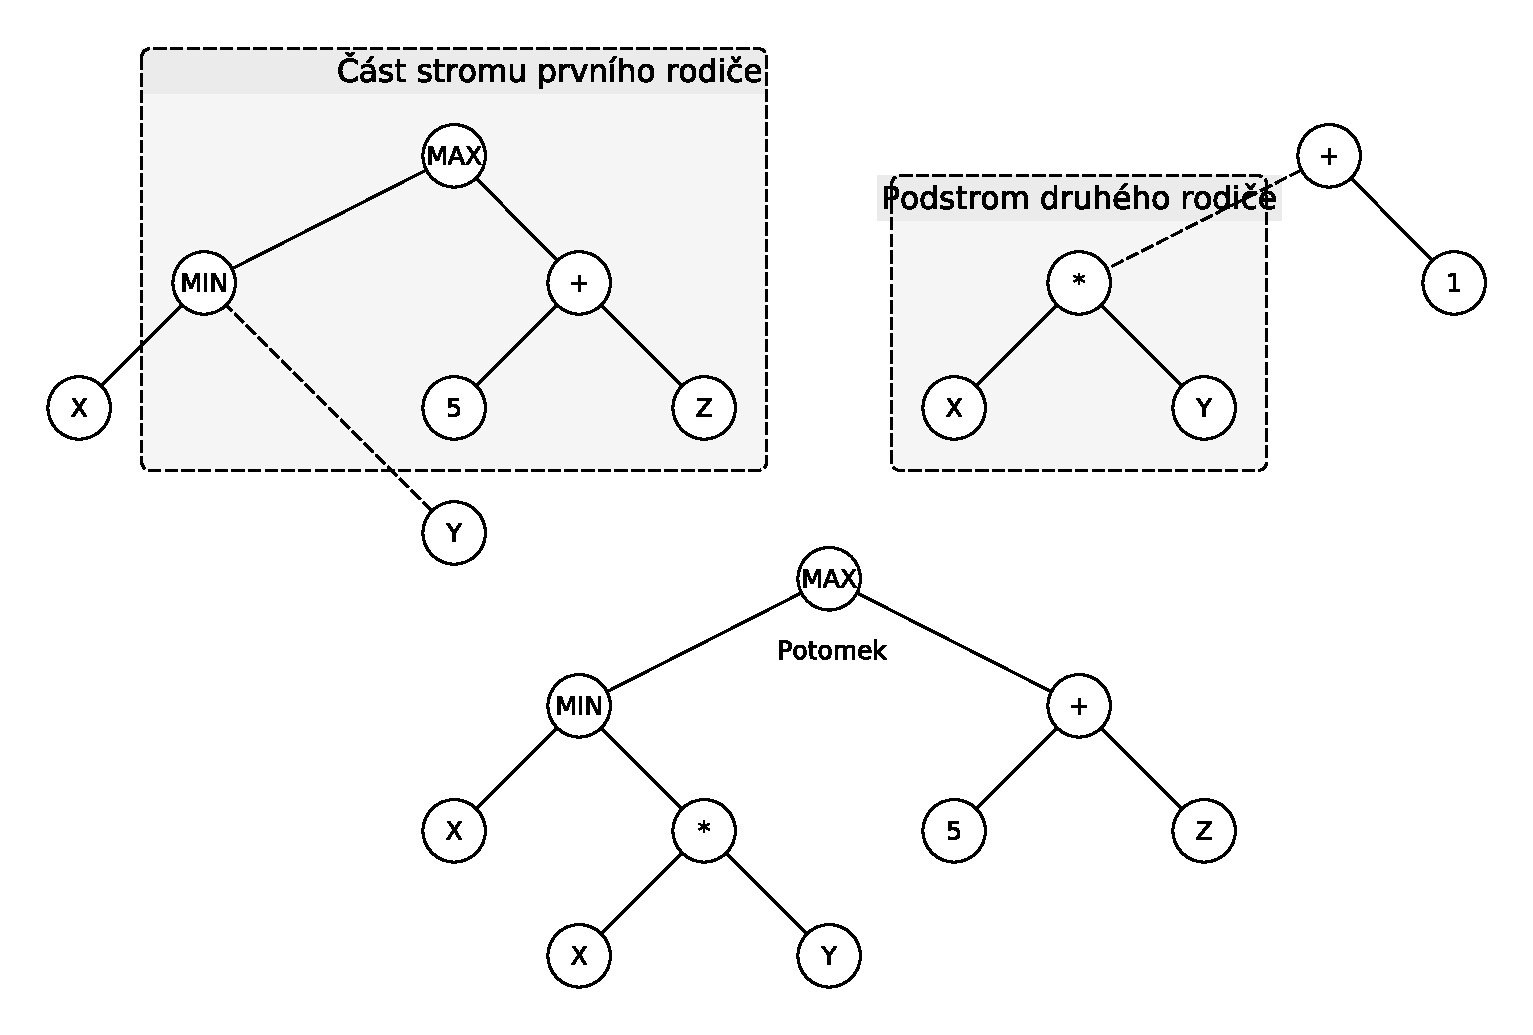
\includegraphics[scale=0.6]{fig/tree_crossover}	
	\caption{Uk�zka oper�toru podstromov�ho k���en�}
	\label{fig:tree_crossover}
\end{figure}
%%%%%%%%%%%%% TREE CROSSOVER EXAMPLE 1 %%%%%%%%%%%%%%%

Je vid�t, �e k���en� vytvo�� pouze jednoho potomka. Pro v�ce potomk� cel� proces 
opakujeme. Dale existuje specializace podstromov�ho k���en�, obdoba jednobodov�ho
k��en�, kdy se ur�� v obou rodi��ch stejn� bod k���en� a p�ehozen� koresponduj�c�ch
podstrom�. Je v�ak pot�eba oba strommy proj�t a naj�t spole�n� region, tedy ��st stromu,
kde je mo�n� k���it. Existuj� dal�� varianty jako je k���en� se zachov�n�m kontextu, 
velikost zachov�vaj�c� k���en� a uniformn� k���en�. T�mito se zde zat�m bl��e zab�vat
nebudeme.

Nejb�n�j�� druh mutace je podstromov� mutace. Algoritmus podstromov� mutace ve stromu
n�hodn� zvol� v�tev z n�� n�hodn� vygeneruje nov� podstrom, jak ilustruje diagram
\ref{fig:subtree_mutation}. V p��pad� tohoto algoritmu jde v podstat� o alternativu k
podstromov�mu k���en� s jedn�m rodi�em a jedn�m n�hodn� generovan�m stromem.

Dal�� variantou mutace v genick�m programov�n� je uzlov� nutace, kdy na ka�d�
uzel stromu je s ur�itou nizkou pravd�podobnost� mutace aplikov�na. Star� uzly
se nahrazuj� nov�mi se stejnou aritou.

%%%%%%%%%%%%% SUBTREE MUTATION EXAMPLE 1 %%%%%%%%%%%%%%%
\begin{figure}[!ht]
	\centering
	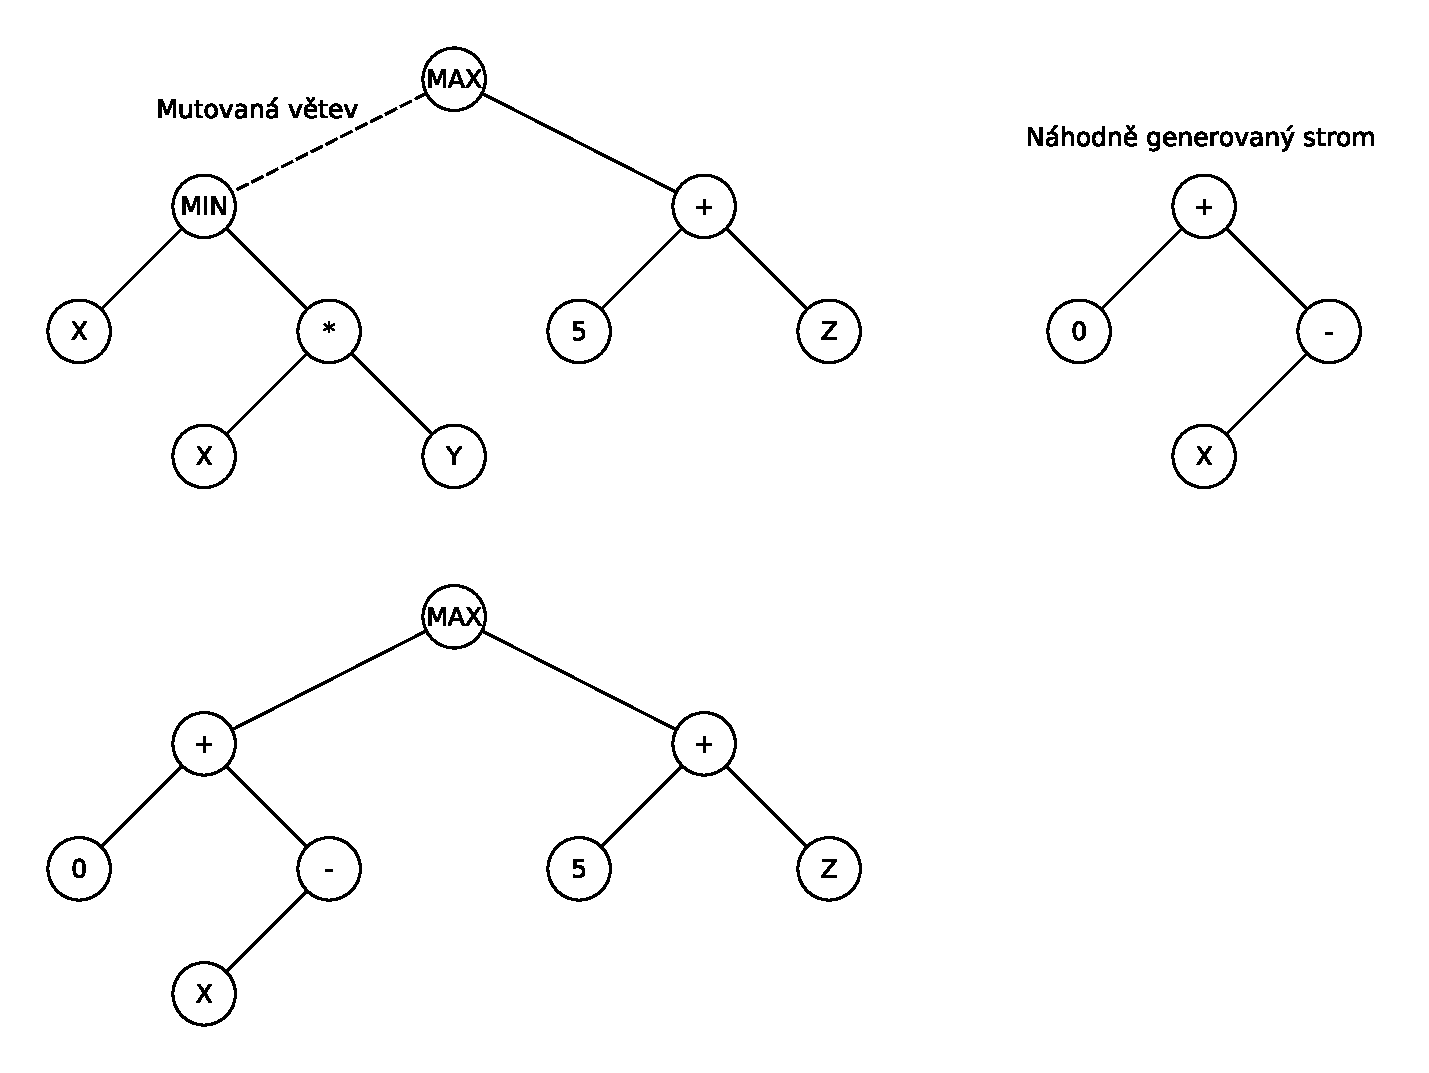
\includegraphics[scale=0.6]{fig/subtree_mutation}	
	\caption{Uk�zka oper�toru podstromov� mutace}
	\label{fig:subtree_mutation}
\end{figure}
%%%%%%%%%%%%% SUBTREE MUTATION EXAMPLE 1 %%%%%%%%%%%%%%%

\subsection{Fitness funkce}
Populace v genetick�m programov�n� jsou programy. Evaluace kvality programu se prov�d�
zpravidla spu�t�n�m dan�ho programu nad dan�m vstupem a ohodnocen�m v�stupu. Spu�t�n� 
programu nad zadan�m vstupem m��eme ch�pat jako zobrazen� z mno��ny genotyp� do mno�iny
fenotyp� za vstupu dal��ho parametru. Cel� proces evaluace m��e b�t tedy ch�p�n jako :
$$ f_{eval} = f \circ f_{run}(input)$$
kde $f$ je standarn� fitness funkce a $f_{run} : I \to (U \to \mathcal{F})$ je
modifikovan� zobrazen� genotyp-fenotyp pro n�jak� vstup $I$.

Fitness funkce v p��pad� genetick�ho programov�n� se li�� od t� tradi�n� v jednom
d�le�it�m sm�ru. Proto�e pracujeme nad programy, mus�me poskytnout zp�sob, jak dan�
program spustit. Mo�nost� by bylo program zkompilovat. To s sebou nese zna�nou re�ii
a tak toto �e�en� nen� v mnoha p��padech vhodn�. Pokud v�ak bychom dan� program cht�li
evaluovat n�kolikr�t (mnohokr�t), m��e se i toto �e�en� jevit jako vhodn�.

�ast�j�� je ale programy interpretovat, to znamen� proj�t strom od list� ke ko�enu a 
spo��t�n� hodnoty uzlu za vstupu hodnot jeho n�sledn�k�. Kostru algoritmu bude jist�
tvo�it pr�chod \textit{postorder}. Evaluace jednotliv�ch hodnot v�ak nemus� b�t za v�ech 
okolnost� trivi�ln�, m��e nap��klad nastat p��pad, kdy bude program d�lit nulou nebo
se sna�it se��st hodnoty r�zn�ch typ� (nap�. \texttt{Bool} a \texttt{Int}). P�i reprodukci
jedinc� zde nar��me na podobn� probl�my jako nap��klad v teorii typ�. Typovost se v
p��pad� genetick�ho programov�n� �e�� dv�ma z�kladn�my zp�soby:

\begin{enumerate}
	\item \textit{typov� unifikace}, kdy ve�ker� uzly i listy stromu budou t�ho� typu,
	\item \textit{siln� typovost}, kdy sou��st� ka�d�ho uzlu i listu stromu bude uveden
	explicitn� jeho typ.
\end{enumerate}

Typov� bezpe�nost je nutn� zejm�na kv�li oper�toru k���en� a mutace. V prvn�m p��pad�
mus�me tedy po��tat s t�m, �e jak�koli podstrom m��e b�t zav�en jako argument
libovoln� funkci z mno�ny $F$ a v�sledn� program p�esto mus� b�t interpretovateln�.
Jin�mi slovy navratov� typ libovoln� funkce z mno�iny $F$ mus� b�t stejn� jako
typ libovoln�ho vstupn�ho argumentu jak�koli dostupn� funkce. Toho m��eme dos�hnout
nap��klad jednodu�e t�m, �e v�echny funkce z mno�iny $F$ budou definov�ny nad jedn�m
oborem hodnot toto�n�ho typu. �asto to v�ak nen� mo�n�, proto se mus�me n�kdy uch�lit
nap��klad k implicitn�m typov�m konverz�m.

Druhou mo�nost� je pou�it� siln� typovan�ch strom�. Tento zp�sob je obecn�j��, nebo�
n�m umo��uje pou��t naprosto libovolnou mno�inu funkc� $F$. Je v�ak tak� v�razn�
implementa�n� slo�it�j��. Ve�ker� reproduk�n� operace zde mus� prov�d�t explicitn�
typovou kontrolu a �astokr�t dlouho proch�zet strom, ne� naleznou uzel vhodn� ke 
k���en� �i mutaci. To m� dopad samoz�ejm� hlavn� na �asovou slo�itost, kter� je 
vy��� ne� v p��pad� typov� unifikace.

Spole�nou vlastnost�, kterou je nutn� splnit jak v p��pad� siln� typovosti, tak v p��pad�
typov� unifiace je, abychom se vypo��dali s mo�n�mi
nedefinovan�mi hodnotami, kter� jsou typick� pro vstupy n�kter�ch parci�ln�ch funkc�
jako je d�len�, kde hodnota je nedefinovan� pokud je d�litel roven nule.
S parci�ln�mi funkcemi se m��eme vypo��dat t�m, �e je explicitn� roz����me na funkce
tot�ln� nebo v p��pad�, je-li nedefinovan� hodnota detekov�na, zna�n� sn���me jedinc�v 
fitness.

\chapter{N�vrh �e�en�}
\label{sec:solution_design}

Jak ji� bylo �e�eno v kapitole \ref{sec:hashing}, navrhujeme-li ha�ovac� funkci "na
m�ru" n�jak�mu konkr�tn�mu univerzu kl���, m��eme dos�hnout podstatn� lep�� 
v�konnosti ha�ovac� funkce, ne� je tomu v p��pad� obecn�ch ha�ovac�ch funkc�.

\section{Probl�m}
Na�im probl�mem bude navrhnout konkr�tn� ha�ovac� funkci pro ha�ov�n� dom�ny
\texttt{IP} adres. Adresa \texttt{IP} je ��slo, jednozna�n� identifikuj�c� s��ov�
rozhran� v s�ti, kter� pou��v� internetov� protokol \texttt{IP}. Vzhledem k tomu,
�e budeme ha�ovat ��sla, nab�z� se ot�zka, zda by nebylo vhodn� pou��t tabulku
s p��m�m p��stupem, tedy pou��t \texttt{IP} adresy pro p��stup do tabulky
p��mo bez vyu�it� ha�ov�n�. Bohu�el nezn�me konkr�tn� interval nebo podmno�inu
univerza \texttt{IP} adres a cel� univerzum je p��li� velk� na to, aby jeho 
prvky mohly slou�it jako ��sla slot� do tabulky. Ve verzi 4 se jedn� o 32 
bitov� ��slo a verzi 6 dokonce o velikosti 128 bit�. Tabulka by tedy musela
m�t $2^{32} = 4 294 967 296$ slot� v p��pad�  \texttt{IP} verze 4 a ve verzi 6
dokonce $2^{128} \approx 3�10^{38}$
slot�. Je vid�t, �e tabulky by byly opravdu velk� a jejich pam�ov� n�ro�nost
by byla nedostupn� i pro specializovan� po��ta�e, uva�ujeme-li, �e by takov�
stroj m�l d�lat i n�co jin�ho, ne� uchov�vat tak ohromnou tabulku. Mus�me se
tedy uch�lit k n�vrhu ha�ovac� funkce.

Pracujeme nad cty�mi datasety, kde ka�d� dataset obsahuje pr�v� 8192 r�zn�ch 
IP adres. Pro ka�d� dataset bude nutno navrhnout zvl�tn� ha�ovac� funkci a tu
na dan� vstupy natr�novat. Nenavrhujeme obecn�j�� ha�ovac� funkci, kter� by dob�e
pracovala nad libovolnou podmno�inou cel�ho univerza IP adres, ale velmi
specifick� funkce, kter� budou dob�e pracovat pr�v� nad zvolen�m datasetem.
Proto�e cel� ha�ovan� prostor je p�edem zn�m, sna��me se naj�t takov� ha�ovac�
funkce, kter� pojmou co nejv�ce z dan� podmno�iny. State of the art �e�en� je v
tomto p��pad� takov� ha�ovac� funkce, kter� pojme cel� podprostor, jej� 
faktor zat��en� bude roven pr�v� jedn� ($\alpha = 1$). Takov� �e�en� v�ak
bude t�k� naj�t. Pro na�e ��ely posta��, nalezneme-li takov�, kter� budou
pracovat l�pe, ne� obecn� ha�ovac� funkce, vytvo�en� �lov�kem. Je zde samoz�ejm�
mo�nost pou��t metody perfektn�ho ha�ovan� \cite{perfect_hashing}, ale to nemus�
b�t ve v�ech p��padech nap��klad z d�vod� pou�it� na specializovan�m hardware
dostupn� mo�nost. Zab�vat se j� tedy nebudeme.


\section{Princip}
Ha�ovac� funkce budeme navrhovat evolu�n�my algoritmy, konkr�tn� za pou�it� 
genetick�ho programov�n�. Zvoleno bylo genetick� programov�n�, proto�e 
jako jedince populace abstraktn� syntaktick� stromy. Jenotliv� syntaktick� 
stromy budeme interpretovat nad zadan�mi vstupy. Ohodnocen� konkr�tn�ho jedince
bude spo��vat v naha�ov�n� jednoho cel� subsetu. Na v�stupu budeme m��it, kolik 
r�zn�ch kl��� dok�zala ha�ovach tabulku obs�hnout kl���.

\section{P�inos pr�ce}
Evolu�n� n�vrh ha�ovac�ch funkc� byl se uk�zalo jako zaj�mav� t�ma v posledn�m 
desetilet� \cite{dobai0,NCHF_auto_design,grammar_evolution,safdari}.
Naprost� v�t�ina prac� se se zam�rovala na n�vrh obecn�ch ha�ovac�ch
funkc�. Byly pou�ity jak evoul�n� n�vrh tak evolu�n� optimalizace. Jedna z prac�
podobn� t� na�� je \cite{safdari}. Je podobn� ve smyslu c�le a pou�it� techniky,
av�ak autor zde pou�il evolu�n� optimalizaci nam�sto n�vrhu. Autor zde optimalizuje
parametry $a,b$ n�sleduj�c� ha�ovac� funkce:
$$h_{a,b}(k) = ((ak + b) \; mod \; p) \; mod \; N$$
kde $p$ je n�jak� prvo��slo a $N - 1$ je nejv�t�� index slotu ha�ovac� tabulky.
``V�sledky jsou slibn�, ale pou�it� metodika je sporn�'' \cite{NCHF_auto_design}.
Proto�e mno�ina kl��� je obsahuje cel� �isla a je volena n�hodn�, n�sk�ta se ot�zka,
pro� v�bec evolvovat ha�ovac� funkci, kdy� mohou b�t pou�ity jej� prvky k indexov�n�
nap��mo. Druh� v�c je, �e autor pou��va jako prim�rn� metriku fitness funkce odolnost
v��i koliz�m, kter� je siln� z�visl� na vstupn� mno�in�. Funkce tedy nemus� dob�e 
zobec�ovat.

Vhodn�j�� metrikou pro n�vrh obecn�ch ha�ovac�ch funkc� je lavinov� efekt, kter� 
nen� z�visl� na vstupu. Tohoto faktu vyu�ili auto�i dal�� podobn� pr�ce \cite{NCHF_auto_design}
zab�vaj�c� se n�vrhem ha�ovac�ch funck�. Tato pr�ce je pravd�podobn� nejbl��e t� 
na�� s rozd�lem, �e my nenavrhujeme obecn� ha�ovac� funkce. Auto�i stejn� jako my,
zvolili genetick� programov�n� jako evolu�n� platformu a volili i podobn� parametry.
Jako z�klad pro svoji fitnes funkci zvolili lavinov� efekt, kter� nen�
z�visl� na vstupu. Funkce navr�en� jej�ch syst�mem otestovali na r�zn�ch vstupn�ch t��d�ch
a dos�hli slibn�ch v�sledk�. Tvrd�, �e jeji algoritmus je velice robustn�, proto�e zm�ny
kl��ov�ch parametr� maj� jen velmi n�zk� nebo ��dn� dopad na v�sledn� funkce. Bohu�el
sou��st� jejich experimentu nen� porovn�n� s algoritmem n�hodn�ho prohled�v�n�, ke 
kter�mu mohl jejich syst�m nedopat�en�m degradovat a kter� je z povahy v�ci tak� 
velmi robustn�. Auto�i tak� tvrd�, �e evolu�n� navrhuj� ha�ovac� funkce, co� 
vzhledem k tomu, �e navrhuj� kompresn� funkce Merkle-Damg\r{a}rdova sch�mata
nen� �pln� pravda. Takov� p��stup se nach�z� na pomez� evolu�n�ho n�vrhu a optimalizace.

Zaj�mavou prac�, kter� se vydala p��stupem kart�zsk�ho genetick�ho programov�n� je
\cite{dobai0}. Kart�zsk� genetick� programov�n� je zejm�na vhodn� pro aplikace bl�zk�
hardwarov� vrstv�, tak�e jeho volba se zd� velmi dobr� vzhledem k c�lov� aplika�n� dom�n�
, kterou jsou s��ov� prvky. Nesporn� p��nos pr�ce spo��v� v pou�it� Kuka���ho ha�ov�n�, kter�
je pou�ito za ��elem zv��en� faktoru zat��en� v�sledn� ha�ovac� tabulky a pr�ce tak dos�hla velmi
dobr�ch v�sledk�. Faktor, kter� tato a na�e pr�ce sd�l� je n�vrh dom�nov� specifick� ha�ovac� 
funkce, kde ha�ovanou dom�nou jsou tak� IP adresy. Pr�ce se v�ak rozch�z� zejm�na ve volb� 
fitnes funkce. Zat�mco my (jak uvid�me pozd�ji v t�to kapitole) jsme zvolili p��stup, kdy ha�ujeme
cel� dan� rozsah a m���me v�skyt kolizi, m��� po�et �sp�n� naha�ovan�ch adres a� do v�skytu
prvn� kolize. Takov� metrika je vskutku zaj�mav�, ale intuitivn� se nask�ta �vaha, �e fitnes funkce
velmi �patn� ohodnot� �e�en�, kter� maj� kolizi velmi brzo, ale p�itom mohou naha�ovat velkou ��st
cel�ho rozsahu. Fitnes funkce jasn� m��� na c�l naha�ovat cel� rozsah (tedy optim�ln� �e�en�), toho
nicm�n� nedos�hla. Bude zaj�mav� porovnat v�sledky na�� prace s s v�sledky dosa�en�mi v t�to
pr�ci. Auto�i op�t pou��vaj� Merkle-Damg\r{a}rdovo sch�ma a pr�ce se tud�� tak� nach�z� na 
pomez� evolu�n�ho n�vrhu a evolu�n� optimalizace.

\section{N�vrh fitness funkce}

V na�� pr�ce navrhujeme specifickou
ha�ovac� funkci pro specifick� univerzum hodnot. Proto m��eme pou��t jako krit�rium
kvality odolnost v��i koliz�m, kter� je nep��m�m ukazatelem toho, jak dob�e funkce
n�hodn� distribuuje sv� v�stupy. Evaluovanou ha�ovac�
funkci budeme testoat nad v�emi prvky univerza. To znamen�, �e budeme navrhovat
celkem cty�i ha�ovac� funkce, pro ka�d� vsupn� dataset jednu. Kdybychom pro v�echny �ty�i
datasety navrhovali jednu jedinou, nedostali bychom dobr� v�sledky. V�sledn� ha�ovac� tabulka
by m�la 8192 slot�, ale byla by ``natr�nov�na'' nad v�emi adresami ze v�ech dataset�. Navic 
bychom se museli zab�vat vhodnou volbou tr�novac�ch dat, co� je obt��n� �kol a nav�c p��dat
krit�rim, kter� by bralo v �vahu zobec�ov�n�. V�sledn� ha�ovac� funkce by ji� nebyla obecn�, ale
n�kde ``na p�l cesty'' mezi obecnou a velmi specifickou ha�ovac� funkci.

Nem�n� d�le�it�m krit�riem je rychlost ha�ovac� funkce a to obzvl�t� v aplikac�ch jako jsou
s��ov� sm�rova�e nebo jin� uplat��n� n�ro�n� na rychlost a odezvu. Jak uvid�me pozd�ji v t�to
kapitole, ve�ker� n�mi navr�en� funkce jsou implicitn� rychl�, proto�e explicitn� omez�me hloubku
abstraktn�ch syntaktick�ch strom� a vhodn� zvol�me mno�inu termin�l� a netermin�l�. 

\section{Zvolen� parametry genetick�ho programov�n�}

V t�to sekci uvedeme, jak� parametry jsme zvolili parametry pro genetic� programov�n�.

\subsection{Genetick� oper�tory a selekce}

Oper�tory mutace pou�ijeme ve dvou verz�ch. \textit{Podstromovou} mutaci a 
\textit{bodovou} mutaci z�rove�. Budeme n�hodn� volit mezi ob�ma alternativami, 
av�ak pravd�podobnost mutace ponech�me velmi n�zkou. P�vodn� implementace algoritm�
genetick�ho programov�n� \cite{GPTutorial} oper�tor mutace vynech�valy �pln�. 
Budeme rad�ji volit cestu postupn� pomaleji konverguj�c� evoluce, ne� abychom 
n�jak� �e�en� minuli.

Co se k���en� t�ka, v prvn�ch verz�ch pou�ijeme z�kladn� formu tedy \textit{podstromov�}
k���en�, pozd�ji jej m��eme porovnat i s pokro�ilej��mi technikami jako jsou 
\textit{jednobodov�} a k���en� se zachov�n�m kontextu. 

Selekci pou�ijeme turnajovou a to zejm�na kv�li sv� determiniti�nosti (jedince
sice mus�me volit n�hodn�, ale nemus�me se mezi nimi stochastiky rozhodovat). Dal��m d�vodem
je dobr� �k�lovatelnost selek�n�ho tlaku.

Po��te�n� populaci budeme generovat n�hodn� bez pou�it� jak�chkoli heuristik
a to metodou \textit{ramped-half-and-half}, kter� zaji��uje pro start algoritmu
kvalitn� populaci co se r�znorodosti verlikost� a tvar� jedinc� t�k�. 

\subsection{Mno�ina termin�l� a funk�n�ch symbol�}

Mno�inu vstup� zkonstruujeme z konstant a vstupn�ch prom�nn�ch. Vstupn�
prom�nn� vyrob�me z jednotliv�ch oktet� adres a budeme po�adovat, aby ka�d�
vstupn� program obsahoval v�echny prom�nn� alespo� jednou, tedy aby pracoval
s celou adresou. Jako konstanty budeme volit prvo��sla. 

Prvo��sla hraj� d�le�itou roli p�i operaci modulo. Pokud vol�me jako argument modula n�jak�
n�sobky mal�ch ��sel jako je nap��klad �islo dv�, m��e se st�t, �e funkce bude
m�t tendenci seskupovat ��sla d�liteln� dv�mi. Jako konstanty budeme volit
prvo��sla z rozsahu $\langle 2, 2N \rangle$, kde $N$ je velikost datasetu. Prvo��sla
budeme implementovat ve form� \textit{pom�jiv� n�hodn� konstanty} (angl. \textit{ephemeral
random constant}, zkr. \textit{ERC}), kterou budeme zna�it $\Re$. Tento p��stup n�m
zajist� vhodn� chov�n� konstany s ohledem na oper�tory k���en� a mutace a tak� p�i
evaluaci. Takov� konstanta pokud je vygenerov�na bude p�i ka�d�m ohodnocen� 
nab�vat stejn� hodnoty, ale v mutaci jej bude m�nit s ur�itou pravd�podobnost� na
n�jak� nejbli��� prvo��slo. 

Ka�d� IP adresa m� d�lku 32 bit� a skl�d� se ze �ty� osmibitov�ch oktet�. Oktety zahrneme
do na�� mno�iny termin�ln�ch symbol� ka�d� zvlṻ a ozna��me je $o_0 \ldots o_4$ jemn�j�� 
d�len� (nap��klad 4, 2 nebo 1 bit) nebudeme uva�ovat, proto�e pou�ijeme rotace (viz. d�le),
kter� budou schopny vybrat jednotliv� bity z oktetu.

Budeme-li uva�ovat Merkle-Damg\r{a}rdovo sch�ma, mus�me reprezentovat v na��
mno�in� termin�l� meziv�sledky kompresn� funkce. I kdy� se jedn� obecn� o iterativn�
sch�ma pracuj�c� nad libovolnou d�lkou vstupu, my si vzhledem k p�edem pevn� 
dan� d�lce 32 bit� vysta��me se cty�mi kompresn�mi jednotkami, jejich� meziv�sledky
budeme zna�it $a_0, a_1, a_2$ (pozn.v p��pad� $a_3 $ se jedn� o v�stup). 

Mno�inu funkc� zvol�me z b�n�ch operac�. Vyhneme se cykl�m a jin�m slo�it�m
��d�c�m konstrukc�m, nebo� ty by vzhledem ke stochastick� povaze algoritmu mohly
vy�stit ve velmi pomal� ha�ovac� funkce. Dal�� nev�tanou skupinou operac� jsou operace
v plovouc� ��dov� ��rce, kter� na procesorech s komplexn� instruk�n� sadou vy�aduj�
mnoho takt� procesoru a�� implementaci v hardware zase zab�raj� velk� m�sto na �ipu.
Nosnou ��st mno�iny funkc� budou tvo�it aritmetick� operace. Konkr�tn� do n� zahrneme
n�soben� ($*$), s��t�n� ($+$), od��t�n� ($-$) a operaci modulo ($mod$). V p��pad� d�len�
se spokoj�me s d�len�m beze zbytku ($/$). Pou��vat budeme tak� booleovsk� operace,
kam zahrneme logick� sou�et ($OR$), logick� sou�in ($AND$) a negaci ($NOT$), kter� 
je d�le�it� zejm�na proto, proto�e umo��uje vytvo�it �plnou b�zi a logick� funkce mohou
tedy zkonstruovat libovolnou logickou funkci. Posledn� skupinu budou tvo�it funkce bitov�.
Zde zahrneme pravou ($\ggg$) a levou ($\lll$) rotaci. Kter� jsou d�le�it� pro v�b�r 
jednotliv�ch bit� ze vstupn�ch argument�. V��et pou�it�ch funkc� a termin�l�
popisuj� tabulky \ref{tab:function_set_design} a \ref{tab:terminal_set_design}.

%%%%%%%%%%%%% FUNCTION AND TERMINAL SETS %%%%%%%%%%%%%%%
\begin{table}
\begin{center}
\begin{tabular}{ |l|c| }
	\hline
   	Kategorie & Z�stupci \\
  	\hline
  	Aritmetick� celo��seln�  & $\{ +,-,*,/,mo	d \}$ \\
  	Aritmetick�                     & $\{\}$ \\
  	Booleovsk�				      & $\{AND, OR, NOT\}$ \\
  	Bitov�					          & $\{ \lll, \ggg \}$ \\ 	 
  	\hline
\end{tabular}
\caption{Zvolen� mno�ina funkc�}
\label{tab:function_set_design}
\end{center}
\end{table}

\begin{table}
\begin{center}
\begin{tabular}{ |l|c| }
	\hline
   	Kategorie & Z�stupci \\
  	\hline
  	Prom�nn�       & $\{o_0, o_1, o_2, o_3, a_0, a_1, a_2\}$ \\
  	Funkce arity 0 & $\{ \Re \}$ \\	 
  	\hline
\end{tabular}
\caption{Zvolen� mno�ina termin�l�}
\label{tab:terminal_set_design}
\end{center}
\end{table}
%%%%%%%%%%%%% FUNCTION AND TERMINAL SETS %%%%%%%%%%%%%%%

\section{Evolu�n� n�vrh ha�ovac�ch funkc�}
V t�to sekci p�edstav�me princip metody a konkr�tn� podobu navr�en�ho �e�en� pro p��m� evolu�n� 
n�vrh ha�ovac�ch funkc�. P��m� proto, proto�e zde nebudeme uva�ovat z�dn� sch�ma ani koncept
jeho� ��sti bychom evolvovali. Ha�ovac� funkce zde budou reprezentovat p��mo abstraktn� syntaktick�
stromy, s kter�mi pracuje algoritmus genetick�ho programov�n�. Funkce navr�en� touto metodou 
budeme ozna�ovat \textit{IPHash}. Ka�d� jedinec bude pracovat se v�emi oktety IP adresy.
Merkle-Damg\r{a}rdovo sch�ma zde nepou��v�me, tak�e do mno�iny termin�l� nen� t�eba zahrnovat
��dn� symboly reprezentuj�c� meziv�sledky. D�le do mno�iny zahrneme konstantu  $\Re$. Oper�tor
k��en� zvol�me v podstromov� variant� a oper�tor mutace takt�. Hloubku jednotliv�ch jedinc� omez�me
na hodnotu �est a to ze dvou d�vodu. Jednak proto�e o�ek�v�me od na�ich ha�ovac�ch funkc� aby byly
rychl� a tak� proto, �e algoritmus genetick�ho programov�n� je pam�ov� n�ro�n� a s rostouc� hloubkou
strom� roste exponenci�ln� pam�ov� n�ro�nost, co� klade ne�nosn� n�roky na v�po�etn� za��zen� 
(servery \textit{edesign1} \ldots \textit{edesign4}). Parametry z�kladn� variantu t�to metody shrnuje 
tabulka \ref{tab:IPHash_params}.

\begin{table}[h]
	\centering
	\caption{Kompletn� shrnut� parametr� genetick�ho programov�n� pro experimenty spjat� s touto sekc�.}
	\begin{tabular}{lc} \\ \hline
		Parametr & Hodnota \\ \hline
		Po�et populac� v b�hu & 1 \\
		Velikost populace & 512 \\
		Reprezentace jedince & jeden abstraktn� syntaktick� strom \\ \hline
		Maxim�ln� po�et ohodnocen� & 100000 \\
		Maxim�ln� hloubka & 6 \\
		Mno�ina funkc� & $\{*, +, \wedge, \ggg\}$ \\
		Mno�ina symbol� & $\{o_{0} .. o_{3}, \Re \}$ \\
		\hline 
		Inicializa�n� metoda & Ramped half-and-half \\
		Po��te�n� maxim�ln� hloubka & 6 \\
		Po��te�n� maxim�ln� hloubka & 2 \\
		\hline
		Selekce & Turnajov� \\
		Velikost turnaje & 7 \\
		\hline
		K���en� & Podstromov� \\
		�etnost selekce ko�ene & 0.0 \\
		�etnost selekce listu & 0.1 \\ 
		�etnost selekce uzl� & 0.9 \\
		\hline 
		Mutace & Podstromov� \\
		�etnost & 0.1 \\
		\hline
		Elitismus & Ano \\
		�etnost & 0.05 \\
		\hline
	\end{tabular}
	\label{tab:IPHash_params}
\end{table}

\section{Optimalizace za pou�it� Merkle-Damg\r{a}rdova sch�matu}

D�le se budeme zab�vat evolu�n�m n�vrhem kompresn�ch funkc� pro Merkle-Damg\r{a}rdovo sch�ma.
Budeme zkoumat dva r�zn� p��stupy. V prvn�m p��pad� budeme evolvovat jednu jedinou kompresn� 
p�i konstrukci Merkle-Damg\r{a}rdova sch�matu tak jak bylo pops�no v kapitole \ref{sec:hashing}.
V druh�m p�ipad� budeme nam�sto jedn� kompresn� funkce evolvovat hned cty�i, pro ka�d� oktet
ha�ovac� funkce jednu jak je uk�z�no na obr�zku \ref{fig:merkle_damgard_2}. Tento p��stup n�m
umo�n� dekomponovat prohled�vac� prostor a dos�hnout tak lep��ch v�sledk� d�ky navr�en�
kompresn�ch funkc� na m�ru konkr�tn�mu oktetu IP adresy. Merkle-Damg\r{a}rdovo sch�ma je obecn�
iterativn� sch�ma p�ij�mat vstup o libovoln� velikosti. My vyu�ijeme v obou p��padech faktu, �e d�lku
vstupu p�edem zn�me. Omez�me se tedy pouze na cty�i kompresn� funkce, pro ka�d� oktet vstupu jednu.
A proto�e je velikost vstupu n�sobek osmi, nemus�me posledn� oktet dopl�ovat o ohrani�uj�c� vatu. D�le
n�me nez�le�� na kryptografick� bezpe�nosti, m��eme tedy vzpostit posledn� kompresn� komponentu
pro d�lkov� ohrani�en�. Ani dobrovolnou finaliza�n� komponentu nevyu�ijeme. V�sledn� ha�ovac� funkce
bude tvaru
$$f_{Merkle-Damgard} : IV \times X \to \{0,1,2 \ldots 8192\}$$,
kde $IV$ je n�jak� cel� ��slo a $X$ je vstupn� IP adresa.

Druh� bude vy�adovat z�sadn� zm�nu v reprezentaci jedinc�. Ka�d� jedinec se bude skl�dat ze cty� 
r�zn�ch abstraktn�ch syntaktick�ch strom� reprezentuj�c� jednotliv� kompresn� funkce. Genetick� oper�tory
mutace a zejm�na k���en� pracuj� v ka�d�m procesu reprodukce pouze nad jedn�m abstraktn�m
syntaktick�m stromem. Proto�e nar�z pracujeme se �ty�mi stromy zvedme po�et evaluac� cty�n�sobn� na
400 000 evaluac�, abychom dos�hli ekvivalentn� situace v porovn�n� s ostatn�mi metodami. V procesu
reprodukce jsou abstraktn� syntaktick� stromy vyb�r�ny n�hodn�. 

\begin{figure}[!ht]
\begin{subfigure}[b]{0.49\textwidth}
%	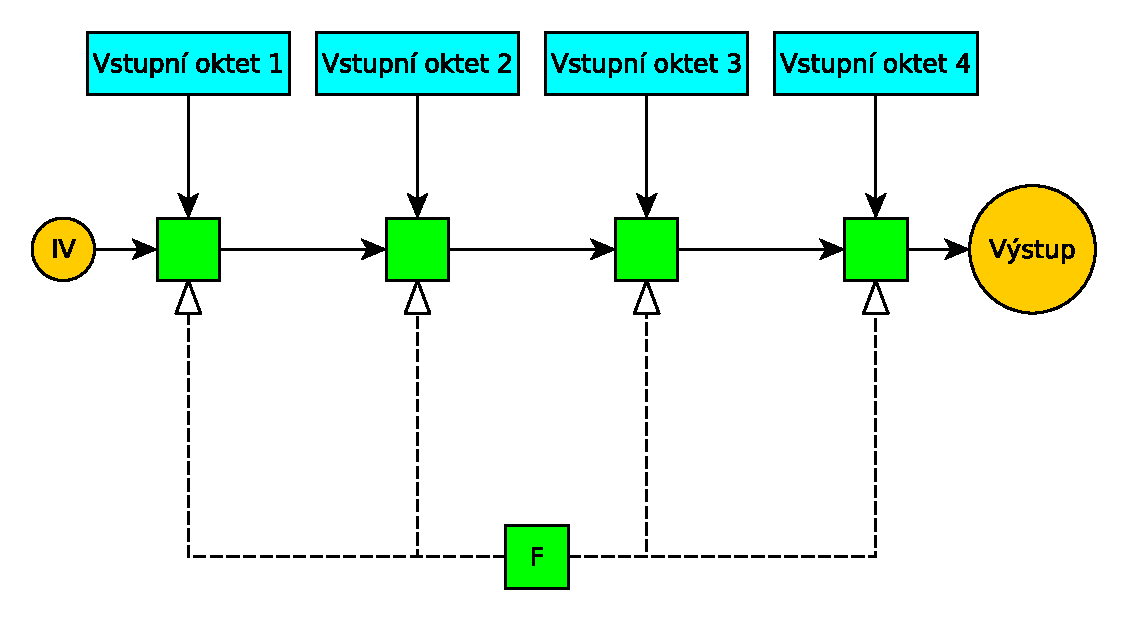
\includegraphics[width=\textwidth]{fig/merkle_damgard_design1}
	\caption{Prvn� p��pad, kter� budeme studovat. Sch�ma pou��v� z�et�zen� jedin� kompresn� funkce.}
\end{subfigure}
\begin{subfigure}[b]{0.49\textwidth}
%	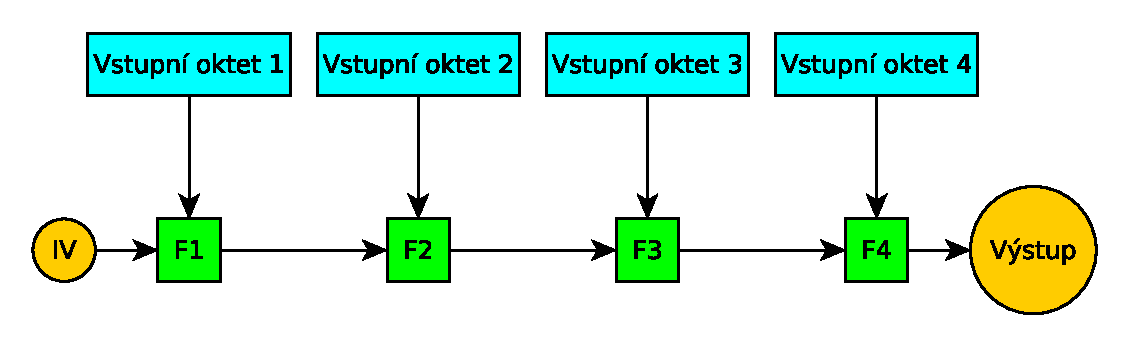
\includegraphics[width=\textwidth]{fig/merkle_damgard_design2}
	\caption{Druh� p��pad, kter� budeme studovat. Sch�ma pou��v� z�et�zen� n�kolika r�zn�ch kompresn�ch funkc�.}
\end{subfigure}
	\caption{Porovn�n� dvou navr�en�ch �e�en� pou��vaj�c� Merkle-Damg\r{a}rdovo sch�ma.}
\end{figure}

U obou variant do tabulky termin�ln�ch symbol� mus�me zav�st p��slu�n� symboly reprezentuj�c�
konkr�tn� meziv�sledky $a_0, a_1, a_2$. Ostatn� parametry se oproti metod� v p�edchoz� sekci neli��.

\section{Evolu�n� n�vrh za pou�it� kuka���ho ha�ov�n�}

\chapter{Experimenty}

%%%%%%%%%%%%% EXPERIMENTS WITH VARIOUS FUNCTIONS %%%%%%%%%%%%%%%
V t�to kapitole provedeme experimenty v nich� nejprve ov���me, zda navr�en� �e�en� poskytuje dobr�
v�sledky. Pot� provedeme dal�� s�rii experiment�, v n�ch� budeme postupn� m�nit parametry navr�en�ho
�e�en� a vyhodnot�me v�sledky. M�nit budeme jak samotn� parametry algoritmu genetick�ho
programov�n�, tak i mno�iny termin�ln�ch a netermin�ln�ch symbol�. Budeme prov�d�t v�dy pouze
jednu zm�nu v ka�d�m experimentu, abychom zachovali jejich v�rohodnost a spr�vnou korespondenci
mezi zm�nou parametru a d�sledkem, jak� m� na v�sledn� �e�en�.

V n�sleduj�c� sekci budeme experimentovat s evolvovan�mi ha�ovac�mi funkcemi, do kter�ch zahrneme
Merkle-Damg\r{a}rdovo sch�ma popsan� v kapitole \ref{sec:hashing}. Kr�tce pop��eme zm�ny v na�em
evolu�n�m algoritmu a provedeme p��slu�n� experimenty.

V posledn� sekci t�to kapitoly uvedeme do n�mi navr�en�ho �e�en� Kuka��� sch�ma jak bylo popsan�
v kapitole \ref{sec:hashing}. Op�t shrneme zm�ny v genetick�m algoritmu, provedeme a vyhodnot�me
p��slu�n� experimenty.

Ve v�ech experimentech budeme m�rit m�ru odolnosti proti koliz�m, konkr�tn� tedy kolik je dan� ha�ovac� 
funkce schopna naha�ovat r�zn�ch IP adres. Dal��, nem�n� d�le�itou roli hraje u ha�ovac�ch funkc� jejich
rychlost. Provedeme tedy i experimenty, kter� odhal� rychlost s jakou jednotliv� ha�ovac� funkce prov�d� svou
�innost. 

\section{Experimenty s navr�en�m �e�en�m}
Nejprve se tedy budeme zkoumat v�sledky, jak� poskytuje n�mi navr�en� �e�en� z kapitoly
 \ref{sec:solution_design}. N�mi navr�en� algoritmus porovn�me se dv�ma variantami n�hodn�ho prohled�v�n�.
 Prvn� varianta bude n�hodn� prohled�v�n� bez pou�it� elitismu, druh� s elitismem. Do grafu zahrneme i jednu
 variantu �lovekem vytvo�en� obecn� ha�ovac� funkce, konkr�tn� ha�ovac� funkci \textit{Murmurhash3} p�edstavenou
 v sekci \ref{sec:evolution_design}. B�hy n�m� navr�en�ho �e�en� jsme prom�tli do graf�, kde ka�d�mu
 datasetu odpov�da jeden graf. Na lev� stran� grafu m��eme vid�t pr�b�hy n�mi navr�en�ho syst�m� a oba
 algoritmy n�hodn�ho prohled�v�n�. Ka�d� k�ivka je v�sledkem medi�nu z pades�t� nez�visl�ch b�h�. Na lev�
 stran� m��eme pozotovat medi�n syst�m� IPHash a u n�j je�t� interval spolehlivosti. Interval spolehlivosti
 je zazna�en dv�ma ohrani�uj�c�my k�ivkami, kde spodn� za�n� prvn� a horn� t�et� kvartil.

%%%%%%%%%%%%% IPHASH AVG Population SET #1 %%%%%%%%%%%%%%%
\begin{figure*}[!ht]
	\centering
	\begin{tikzpicture}
	\begin{axis}[ %
	, name=plot1
	, height=8cm
	, width=0.50\textwidth
	, grid=major
	, xlabel=Generation
	, ymin=5180
	, ymax=5320
	, ylabel=Successfully hashed
	, legend style=
	{ at={(1.0, 0.3)}
		, anchor=east
	}
	]
	\addplot[color=black, dashdotted, thick, mark=none] table {graph/IPHash/Set1/ElitistRandomRun_1.dat};
	\addlegendentry{Elitist Random Search}
	
	\addplot[color=blue, dotted, very thick, mark=none] table {graph/IPHash/Set1/RandomRun_1.dat};
	\addlegendentry{Random Search}
	
	\addplot[color=green, solid, thick, mark=none] coordinates {(0,5190) (194, 5190)};
	\addlegendentry{MurmurHash3}
	
	\addplot[color=red, mark=none, dashed, thick] table {graph/IPHash/Set1/IPHashMedian_1.dat}; 
	\addlegendentry{Proposed IPHash}
	
	\end{axis}
	
	\begin{axis}[ %
	, name=plot2
	, at=(plot1.right of south east)
	, anchor=left of south west
	, ymin=5180
	, ymax=5320
	, height=8cm
	, width=0.50\textwidth
	, grid=major
	, xlabel=Generation
	%%	, ylabel=Successfully hashed
	, yticklabels={,,}
	%%	, legend pos=outer north east
	, legend style=
	{ at={(1.0, 0.3)}
		, anchor=east
	}
	]
	\addplot[color=red, mark=none, dashed,thick] table {graph/IPHash/Set1/IPHashMedian_1.dat}; 
	\addlegendentry{Proposed IPHash}
	\addplot[color=red, mark=none, dotted] table {graph/IPHash/Set1/IPHashReliab1_1.dat}; 
	%\addlegendentry{Proposed IPHash RR1}
	\addplot[color=red, mark=none, dotted] table {graph/IPHash/Set1/IPHashReliab3_1.dat}; 
	\addlegendentry{Diversity of runs}
	\end{axis}
	\end{tikzpicture}
	\caption{Evolvovan� ha�ovac� funkce a jejich fitnes hodnota nad data setem ��slo 1.}
	\label{fig:basicComparison1}
\end{figure*}
%%%%%%%%%%%%% IPHASH AVG Population SET #1 %%%%%%%%%%%%%%%

Na obr�zku \ref{fig:basicComparison1} m��eme vid�t vid�t porovn�n� b�h� a jejich v�sledk� v�ech algoritm�.
Je patrn�, �e nad prvn�m datasetem, navr�en� �e�en� jasn� dominuje nad zb�vaj�c�my algoritmy. IPHash
naha�oval o 25 IP adres v�ce ne� druh� nej�sp�n�j�� algoritmus n�hodn�ho prohled�v�n�. Nejh��e si vedl
�lov�kem vytvo�en� algoritmus \textit{MurmurHash3}, kter� naha�oval o cel�ch 111 IP adres m�n�. 

Z intervalu spolehlivost m��eme usoudit, �e n�mi navr�en� algoritmus skute�n� funguje dob�e a rozptyly jeho
�e�en� nejsou p��li� signifikantn�. Nalezen� �e�en� nen� tedy d�lem ��st� n�hody. Z grafu m��eme vy��st, �e 
algoritmus v prn�ch n�kolika generac�ch rapidn� konverguje a s postupn�m p��b�v�n�m generac� se jeho 
konvergence zpomaluje. Toto je typickou vlastnost� algoritmu genetick�ho programov�n� \cite{GPTutorial}.

%%%%%%%%%%%%% IPHASH AVG Population SET #2 %%%%%%%%%%%%%%%
\begin{figure*}[!ht]
	\centering
	\begin{tikzpicture}
	\begin{axis}[ %
	, name=plot1
	, height=8cm
	, width=0.50\textwidth
	, grid=major
	, xlabel=Generation
	, ymin=5180
	, ymax=5330
	, ylabel=Successfully hashed
	, legend style=
	{ at={(1.0, 0.3)}
		, anchor=east
	}
	]
	\addplot[color=black, dashdotted, thick, mark=none] table {graph/IPHash/Set2/ElitistRandomRun_2.dat};
	\addlegendentry{Elitist Random Search}
	
	\addplot[color=blue, dotted, very thick, mark=none] table {graph/IPHash/Set2/RandomRun_2.dat};
	\addlegendentry{Random Search}
	
	\addplot[color=green, solid, thick, mark=none] coordinates {(0,5190) (194, 5190)};
	\addlegendentry{MurmurHash3}
	
	\addplot[color=red, mark=none, dashed, thick] table {graph/IPHash/Set2/IPHashMedian_2.dat}; 
	\addlegendentry{Proposed IPHash}
	
	\end{axis}
	
	\begin{axis}[ %
	, name=plot2
	, at=(plot1.right of south east)
	, anchor=left of south west
	, ymin=5180
	, ymax=5330
	, height=8cm
	, width=0.50\textwidth
	, grid=major
	, xlabel=Generation
	%%	, ylabel=Successfully hashed
	, yticklabels={,,}
	%%	, legend pos=outer north east
	, legend style=
	{ at={(1.0, 0.3)}
		, anchor=east
	}
	]
	\addplot[color=red, mark=none, dashed,thick] table {graph/IPHash/Set2/IPHashMedian_2.dat}; 
	\addlegendentry{Proposed IPHash}
	\addplot[color=red, mark=none, dotted] table {graph/IPHash/Set2/IPHash1stQ_2.dat}; 
	%\addlegendentry{Proposed IPHash RR1}
	\addplot[color=red, mark=none, dotted] table {graph/IPHash/Set2/IPHash3rdQ_2.dat}; 
	\addlegendentry{Diversity of runs}
	\end{axis}
	\end{tikzpicture}
	\caption{Evolvovan� ha�ovac� funkce a jejich fitnes hodnota nad data setem ��slo 2.}
	\label{fig:basicComparison2}
\end{figure*}
%%%%%%%%%%%%% IPHASH AVG Population SET #2 %%%%%%%%%%%%%%%

V p��pad� druh�ho datasetu jsou dosa�en� v�sledky (\ref{fig:basicComparison2}) je�t� lep��. IPHash dos�hl vy���ho medi�nu
a op�t v�razn� p�ev��il jak n�hodn� prohled�v�n�, tak \textit{MurmurHash3}. Naha�oval o 24
IP adres v�ce ne� n�hodn� prohled�v�n� a o 115 IP adres v�ce, ne� \textit{MurmurHash3}. 
Interval spolehlivosti je s v�jimkou posledn�ch n�kolika generac� v�ce sev�en� kolem k�ivky
IPHash, co� zna�� spolehliv� algoritmus. Stejn� jako v p�edchoz�m p��pad�, algoritmus rapidn�
konverguje v prvn�ch n�kolika generac�ch. Pot� jeho n�stup ust�v�.

%%%%%%%%%%%%% IPHASH AVG Population SET #3 %%%%%%%%%%%%%%%
\begin{figure*}[!ht]
	\centering
	\begin{tikzpicture}
	\begin{axis}[ %
	, name=plot1
	, height=8cm
	, width=0.50\textwidth
	, grid=major
	, xlabel=Generation
	, ymin=5180
	, ymax=5320
	, ylabel=Successfully hashed
	, legend style=
	{ at={(1.0, 0.3)}
		, anchor=east
	}
	]
	\addplot[color=black, dashdotted, thick, mark=none] table {graph/IPHash/Set3/ElitistRandomRun_3.dat};
	\addlegendentry{Elitist Random Search}
	
	\addplot[color=blue, dotted, very thick, mark=none] table {graph/IPHash/Set3/RandomRun_3.dat};
	\addlegendentry{Random Search}
	
	\addplot[color=green, solid, thick, mark=none] coordinates {(0,5206) (194, 5206)};
	\addlegendentry{MurmurHash3}
	
	\addplot[color=red, mark=none, dashed, thick] table {graph/IPHash/Set3/IPHashMedian_3.dat}; 
	\addlegendentry{Proposed IPHash}
	
	\end{axis}
	
	\begin{axis}[ %
	, name=plot2
	, at=(plot1.right of south east)
	, anchor=left of south west
	, ymin=5180
	, ymax=5320
	, height=8cm
	, width=0.50\textwidth
	, grid=major
	, xlabel=Generation
	%%	, ylabel=Successfully hashed
	, yticklabels={,,}
	%%	, legend pos=outer north east
	, legend style=
	{ at={(1.0, 0.3)}
		, anchor=east
	}
	]
	\addplot[color=red, mark=none, dashed,thick] table {graph/IPHash/Set3/IPHashMedian_3.dat}; 
	\addlegendentry{Proposed IPHash}
	\addplot[color=red, mark=none, dotted] table {graph/IPHash/Set3/IPHash1stQ_3.dat}; 
	%\addlegendentry{Proposed IPHash RR1}
	\addplot[color=red, mark=none, dotted] table {graph/IPHash/Set3/IPHash3rdQ_3.dat}; 
	\addlegendentry{Diversity of runs}
	\end{axis}
	\end{tikzpicture}
	\caption{Evolvovan� ha�ovac� funkce a jejich fitnes hodnota nad data setem ��slo 3.}
	\label{fig:basicComparison3}
\end{figure*}
%%%%%%%%%%%%% IPHASH AVG Population SET #3 %%%%%%%%%%%%%%%

Zaj�mav� situace nastala v p��pad� t�et�ho datasetu \ref{fig:basicComparison3}. Na prvn� pohled je patrn�,
�e oba itera�n� algoritmy zde �e�en� s obdobnou hodnotou fitnes. D�le je vid�t,
�e medi�nov� hodnota fitnes se n�m znateln� a to o v�ce ne� dvacet naha�ovan�ch 
adres v p��pad� algoritmu IPHash. V�sledn� �e�en� n�hodn�ho prohled�v�n� na�la
�e�en� s obdobnou hodnotou fitnes jako v p�edchoz�m p��pad�. Naopak se zv��ila 
hodnota u algoritmu \textit{MurmurHash3}, a to o cel�h 15 naha�ovan�ch adres.

Z intervalu spolehlivosti m��eme vy��st, mnohem v�t�� rozptyl ne� v p�edchoz�ch
p��padech. IPHash algoritmus produkuje mnohem v�t�� diverzitu v nalezen�ch �e�en�ch.
Tento fakt ve spojen� s obdobnou hodnotou fitnes funkce jako m� n�hodn� prohled�v�n�
zna��, �e stavov� prostor tak jak modelov�n t�et�m datasetem je vhodn� sp��e pro 
algoritmus n�hodn�ho prohled�v�n�, ne� pro evolu�n� algoritmus. Evolu�n� algoritmus
se v prostoru dostupn�ch �e�en� ``nem� �eho chytit''. Proto �patn� konverguje a jeho
pr�b�h p�ipom�n� n�hodn� prohled�v�n�. Na po��tku algoritmus konverguje velmi rychle
velmi rychle v�ak ztr�c� ve�ker� progres a t�m�� �pln� staguje.

%%%%%%%%%%%%% IPHASH AVG Population SET #4 %%%%%%%%%%%%%%%
\begin{figure*}[!ht]
	\centering
	\begin{tikzpicture}
	\begin{axis}[ %
	, name=plot1
	, height=8cm
	, width=0.50\textwidth
	, grid=major
	, xlabel=Generation
	, ymin=5180
	, ymax=5320
	, ylabel=Successfully hashed
	, legend style=
	{ at={(1.0, 0.3)}
		, anchor=east
	}
	]
	\addplot[color=black, dashdotted, thick, mark=none] table {graph/IPHash/Set4/ElitistRandomSearch_4.dat};
	\addlegendentry{Elitist Random Search}
	
	\addplot[color=blue, dotted, very thick, mark=none] table {graph/IPHash/Set4/RandomSearch_4.dat};
	\addlegendentry{Random Search}
	
	\addplot[color=green, solid, thick, mark=none] coordinates {(0,5206) (194, 5206)};
	\addlegendentry{MurmurHash3}
	
	\addplot[color=red, mark=none, dashed, thick] table {graph/IPHash/Set4/IPHashMedian_4.dat}; 
	\addlegendentry{Proposed IPHash}
	
	\end{axis}
	
	\begin{axis}[ %
	, name=plot2
	, at=(plot1.right of south east)
	, anchor=left of south west
	, ymin=5180
	, ymax=5320
	, height=8cm
	, width=0.50\textwidth
	, grid=major
	, xlabel=Generation
	%%	, ylabel=Successfully hashed
	, yticklabels={,,}
	%%	, legend pos=outer north east
	, legend style=
	{ at={(1.0, 0.3)}
		, anchor=east
	}
	]
	\addplot[color=red, mark=none, dashed,thick] table {graph/IPHash/Set4/IPHashMedian_4.dat}; 
	\addlegendentry{Proposed IPHash}
	\addplot[color=red, mark=none, dotted] table {graph/IPHash/Set4/IPHash1stQ_4.dat}; 
	%\addlegendentry{Proposed IPHash RR1}
	\addplot[color=red, mark=none, dotted] table {graph/IPHash/Set4/IPHash3rdQ_4.dat}; 
	\addlegendentry{Diversity of runs}
	\end{axis}
	\end{tikzpicture}
	\caption{Evolvovan� ha�ovac� funkce a jejich fitnes hodnota nad data setem ��slo 4.}
	\label{fig:basicComparison4}
\end{figure*}
%%%%%%%%%%%%% IPHASH AVG Population SET #4 %%%%%%%%%%%%%%%

Zd� se, �e stejn� jako v p�edchoz�m p��pad�, se IPHash chov� i nad posledn�m datasetem �ty�i (\ref{fig:basicComparison4}).
Medi�nov� hodnota je op�t ni��� ne� v p��pad� n�hodn�ho prohled�v�n�. Je v�ak vy���, ne� v p��pad�
\textit{MurmurHash3}. Stavov� prostor, zda se, m� op�t n�hodnou charakteristiku a algoritmus spatn�
koverguje. Rozptyl je op�t v�t�� ne� v prvn�ch dvou p��padech. Algoritmus rychle konverguje v prvn�ch
n�kolika generac�ch. Brzy v�ak p�ejde ve stagnaci.

D��ve, ne� se pust�me d�le je vhodn� se zamyslet na doposud dosa�en�mi v�sledky algoritmem n�hodn�ho
prohled�v�n�. Teoreticky algoritmus n�hodn�ho prohled�v�n� je takov�, kter� n�hodn� vyb�r� body
dan�ho stavov�ho prostoru. Sou��st� ka�d�ho evolu�n�ho algoritmu je v�ak tak� reprezentace probl�mu,
kter� modeluje stavov� prostor. V na�em p��pad� bylo n�hodn� proheld�v�n� velmi siln� ovlivn�no 
reprezentac� jednc� jako abstraktn�ch syntaktick�ch strom� a pou�it�mi termin�ln�mi a funk�n�mi symboly.
Lze tedy st�le mluvit o algoritmu n�hodn�ho prohled�v�n�, m�jme v�ak na pam�ti, �e v�sledky j�m
dosa�enou jsou velkou m�rou zp�soben� pr�v� n�mi vhodn� zvolenou reprezentac�.

Jedna ze zaj�mav�ch vlastost� spole�nou pro v�echny grafy je fakt, �e v inici�ln�ch populac�ch obou
itera�n�ch algoritm� jsme nalezli �e�en�, kter� p�evy�ovala �lov�kem vytvo�en� ha�ovac� funkce. Toto
je velmi zaj�mav� poznatek. D�vodem je, �e velikost populace jsme zvolili pom�rn� velkou. I p�es to
v�ak z toho plyne, �e po n�kolika m�lo pokusech s n�hodn�m generov�n�m abstraktn�ch syntaktick�ch 
strom� m��eme nal�zt �e�en�, kter� p�evy�uj� ta �lov�kem vytvo�en�.

\begin{table}[!ht]
	\centering
	\begin{tabular}{l|c|c|c|c}
		Ha�ovac� funkce & Dataset 1 & Dataset 2 & Dataset 3 & Dataset 4 \\
		\hline
		FarmHash             & 5227 & 5199 & 5203 & 5158 \\
		MurmurHash3    		 & 5190 & 5190 & 5206 & 5206 \\
		CityHash             & 5180 & 5156 & 5171 & 5155 \\
		\hline
		IPHash               & 5301 & 5305 & 5274 & 5278 \\
		N�hodn� prohled�v�n� & 5276 & 5281 & 5277 & 5281 \\
		\hline
	\end{tabular}
	\caption{Shrnut� v�sledk� evolvovan�ch i obecn�ch ha�ovac�ch funkc� nap��� v�emi datasety.}
	\label{tab:IPHash_conclusion}
\end{table}

Ve shrnuj�c� tabulkce \ref{tab:IPHash_conclusion} m�zeme vid�t v�sledky algoritmu n�hodn�ho prohled�v�n�
a algoritmu IPHash v kontrastu s �lov�kem vytvo�en�mi ha�ovac�mi funkcemi z kapitoly \ref{sec:hashing}.
Nad prvn�mi dv�ma m� nejlep�� medi�novou hodnotu fitnes IPHash. Nad druh�mi dv�ma naopak n�hodn� prohled�v�n�.
�lov�kem vytvo�en� algoritmy ani v jednom p��pad� nap�ekonaly IPHash. Naopak IPHash nad obecn�mi ha�ovac�mi
funkcemi jasn� dominuje. Rozd�l je nejv�ce zn�t v v p��pad� funkce \textit{CityHash} nad datasetem dva, kde se rozd�l
rovn� hodnot� 150 naha�ovan�ch funkc�. Nejm�n� je to naopak v p��pad� funkce \textit{FarmHash} nad datasetem t�i,
kde se rozd�l zmen�il na 71 naha�ovan�ch adres.
 
Nyn� se budeme podrobn�ji zab�vat rozptylem nejlep��ho nalezen�ho �e�en� (ekvivalent
hodnoty posledn� generace algoritmu), kter�  nalezne n�hodn� prohled�v�n� a IPHash v porovn�n� s
algoritmem n�hodn�ho prohled�v�n�.

%%%%%%%%%%%%% IPHASH BOXPLOT %%%%%%%%%%%%%%%
\begin{figure}[!h]
	\centering
	\begin{tikzpicture}
	\begin{axis}
	[ boxplot/draw direction=y
	, name=plot1
	, xtick={1,2,3}
	, xticklabels={RS, IPHash, N�hodn� prohled�v�n�}
	, ymin=5200
	, ymax=5360
	]
	\addplot+[
	boxplot prepared={
		lower whisker=5250,
		lower quartile=5266,
		median=5276,
		upper quartile=5286,
		upper whisker=5311,
	},
	] coordinates {}; % RS
	
	\addplot+[
	boxplot prepared={
		lower whisker=5279,
		lower quartile=5292,
		median=5301,
		upper quartile=5315,
		upper whisker=5352,
	},
	] coordinates {}; % IPHash
	
	\addplot+[
	boxplot prepared={
		lower whisker=5242,
		lower quartile=5265,
		median=5274,
		upper quartile=5286,
		upper whisker=5319,
	},
	] coordinates {}; % ERS
	\end{axis}		

	\begin{axis}
	[ boxplot/draw direction=y
	, name=plot2
	, at=(plot1.right of south east)
	, xtick={1,2,3}
	, xticklabels={RS, IPHash, N�hodn� prohled�v�n�}
	, ymin=5200
	, ymax=5360
	, yticklabels={,,}
	]		
	\addplot+[color=blue,
		boxplot prepared={
		lower whisker=5255,
		lower quartile=5270,
		median=5281,
		upper quartile=5290,
		upper whisker=5331,
	},
	] coordinates {}; % RS
	
	\addplot+[color=red,
		boxplot prepared={
			lower whisker=5286,
			lower quartile=5298,
			median=5305,
			upper quartile=5319,
			upper whisker=5352,
		},
		] coordinates {}; % IPHash
		
	\addplot+[
	boxplot prepared={
		lower whisker=5251,
		lower quartile=5270,
		median=5279,
		upper quartile=5285,
		upper whisker=5328,
	},
	] coordinates {}; % ERS
	\end{axis}		
	\end{tikzpicture}
	\caption{Porovn�n� v�sledk� algirutmu IPHash a n�hodn�ho porovn�n� krabicov�m diagramem pro datasety jedna a dv�.}
	\label{fig:basic_boxplot_1}
\end{figure}

Na dvou krabicov�ch diagramech grafech na obr�zku \ref{fig:basic_boxplot_1}, vid�me porovn�n�
algoritm� v nad datasety jedna dv�. Nad t�mito datasety si algoritmus vedl velmi dob�e, a to potvrzuj�
i krabicov� diagramy. V cel�m rozsahu rozptylu n�mi navr�en�ho �e�en� dost�v�me lep�� v�sledky, ne� u
algoritmu n�hodn�ho prohled�v�n� a to v obou p��padech. Nejlep�� �e�en� nalezen� algoritmem n�hodn�ho
prohled�v�n� je jen nepatrn� v��e, ne� horn� hranice rozptylu algoritmu IPHash. Nejhor�� �e�en� nalezen�
algoritmem IPHash je v p��pad� prvn�ho datasetu lep�� ne� medi�n algoritmu n�hodn�ho prohled�v�n� a
v p��pad� druh�ho datasetu dokonce lep��, ne� nejlep�� �e�en� rozptylu n�hodn�ho prohled�v�n�. Co se t��e
nejlep��ho �e�en� algoritmu IPHash, tak to zna�n� p�evu�uje i to nejlep�� �e�en� nalezen� algoritmem
n�hodn�ho prohled�v�n�. Je tedy patrn�, �e ve v�ech p��padech algoritmus IPHash dob�e konvergoval v dan�m
stavov�m prostoru popsan�m fitnes funkc� a zvolenou reprezentac� jedinc�.

\begin{figure}[!h]
\centering
\begin{tikzpicture}
	\begin{axis}
	[ boxplot/draw direction=y
	, name=plot3	
	, xtick={1,2,3}
	, xticklabels={RS, IPHash, N�hodn� prohled�v�n�}
	, ymin=5200
	, ymax=5360
	]		
	\addplot+[
	boxplot prepared={
		lower whisker=5246,
		lower quartile=5268,
		median=5277,
		upper quartile=5290,
		upper whisker=5302,
	},
	] coordinates {}; % RS
	
	\addplot+[
	boxplot prepared={
		lower whisker=5242,
		lower quartile=5261,
		median=5274,
		upper quartile=5287,
		upper whisker=5342,
	},
	] coordinates {}; % IPHash
	
	\addplot+[
	boxplot prepared={
		lower whisker=5237,
		lower quartile=5263,
		median=5275,
		upper quartile=5289,
		upper whisker=5318,
	},
	] coordinates {}; % ERS
	\end{axis}		

	\begin{axis}
	[ boxplot/draw direction=y
	, name=plot4
	, at=(plot3.right of south east)
	, xtick={1,2,3}
	, xticklabels={RS, IPHash, N�hodn� prohled�v�n�}
	, yticklabels={,,}
	, ymin=5200
	, ymax=5360
	]		
	\addplot+[
	boxplot prepared={
		lower whisker=5251,
		lower quartile=5269,
		median=5281,
		upper quartile=5285,
		upper whisker=5310,
	},
	] coordinates {}; % RS
	
	\addplot+[
	boxplot prepared={
		lower whisker=5252,
		lower quartile=5264,
		median=5278,
		upper quartile=5285,
		upper whisker=5298,
	},
	] coordinates {}; % IPHash
	
	\addplot+[
	boxplot prepared={
		lower whisker=5251,
		lower quartile=5268,
		median=5276,
		upper quartile=5290,
		upper whisker=5323,
	},
	] coordinates {}; % ERS
	\end{axis}		

	\end{tikzpicture}
	\caption{Porovn�n� v�sledk� algirutmu IPHash a n�hodn�ho porovn�n� krabicov�m diagramem pro datasety t�i a �ty�i.}
	\label{fig:basic_boxplot_2}
\end{figure}
%%%%%%%%%%%%% IPHASH BOXPLOT %%%%%%%%%%%%%%%

V kontrastu s v�sledky nad prvn�mi dv�ma datasety jsou v�sledky nad druh�mi dv�ma datasety. V obou p��padech
si n�mi navr�en� �e�en� nevedlo v pr�m�ru l�pe, ne� algorimus n�hodn�ho prohled�v�n�. Je vid�t, �e nejlep��
nalezen� �e�en� maj� obdobn� rozptyl. Nad datasetem ��slo t�i je rozptyl velmi podobn�, t�sn� ve prosp�ch 
n�hodn�ho prohled�v�n�. Medi�n lze pova�ovat za toto�n�. Nejlep�� nalezen� �e�en� v�ak jasn� mluv� ve prosp�ch
algoritmu IPHash, kde je rozd�l v�ce ne� dvacet �sp�n� naha�ovan�ch adres. V p��pad� datasetu ��slo cty�i n�hodn�
prohled�v�n� jasn� p�ed�ilo n�mi navr�en� algoritmus. I p�es to, �e je medi�nov� hodnota n�hodn�ho prohled�v�n�
nepatrn� men��, je zanedbateln� a lze ji pova�ovat za nep�esnost m��en�. Horn� i spodn� hranice rozptylu n�hodn�ho
prohled�v�n� je polo�ena v��e ne� v p��pad� algoritmu IPHash. Celkem lze pozorovat, �e ani jeden algoritmus 
nena�el �e�en�, kter� by mohlo konkurovat nejlep��m v�slek�m dosa�en�m v nad p�ede�l�mi datasety. I p�es to
nejlep�� nalezen� �e�en� jednozna�n� mluv� ve prosp�ch algoritmu n�hodn�ho prohled�v�n�.

Nejlep��ch v�sledk� bylo dosa�eno nad prvn�mi dv�ma datasety, kde v obou p��padech si nejl�pe vedl n�mi navr�en�
algoritmus. U t�et�ho datasetu se v�sledky zhor�ili v porovn�n� s p�edchoz�mi a to u obou algoritm�. Oba si byly 
rovnoc�n�, ale nejlep�� �e�en� nalezl algoritmus IPHash. V p��pad� posledn�ho datasetu jsou v�sledky podobn� jako
v p��pad� datasetu t�i. Nejlep�� �e�en� nalezlo n�hodn� prohled�v�n�, ale i zde m��eme pozorovat zho��en�. 

%%%%%%%%%%%%% IPHASH Population depth %%%%%%%%%%%%%%%
\begin{figure}[!ht]
\centering
\begin{tikzpicture}
	\begin{axis}[ 
	, grid=major
	, width=0.49\linewidth
	, legend pos=outer north east
	, xlabel={Population size}
	, xtick={1,2,3,4,5,6,7,8}
	, xticklabels={8,16,32,64,128,256,512}
	, ylabel={Initial depth}
	, ytick={2,3,4,5,6} 
	, zlabel={Successfully hashed}
	, ztick={5280,5290,5300,5310,5320}
	, zticklabels={5280,5290,5300,5310,5320}
	]
	\addplot3[surf] coordinates {
		    %8            16         32           64           128          256          512          1024  
		    (1,2,5288.5) (2,2,5289) (3,2,5291)   (4,2,5294)	  (5,2,5297)   (6,2,5295)   (7,2,5293.5) (8,2,5296.5)
		    
		    (1,3,5292.9) (2,3,5301) (3,3,5300.5) (4,3,5314)   (5,3,5312.5) (6,3,5310.5) (7,3,5306)   (8,3,5307)
		    
		    (1,4,5299.5) (2,4,5306) (3,4,5305)   (4,4,5308.5) (5,4,5311.5) (6,4,5312)   (7,4,5306.5) (8,4,5309.5)
		    
		    (1,5,5299)   (2,5,5300) (3,5,5307)   (4,5,5313.5) (5,5,5302.5) (6,5,5311)   (7,5,5312)   (8,5,5307)
		    
		    (1,6,5293.5) (2,6,5302) (3,6,5304)   (4,6,5295.5) (5,6,5307)   (6,6,5304)   (7,6,5302)   (8,6,5307) 
		};
	\end{axis}
\end{tikzpicture}
\caption{Number of successfully hashed addresses in relation to population size and initial depth.}
\label{fig:basicPopulationDepth1}
\end{figure}
%%%%%%%%%%%%% IPHASH Population depth %%%%%%%%%%%%%%%

\begin{table}[h]
	\centering
	\caption{Vliv r�zn�ch voleb and termin�ln�ch a netermin�ln�ch mno�in na v�slednou hodnotu fitnes. Experimenty jsou provedeny
		nap��� v�emi datasety.}
	\begin{tabular}{cccccc} \\ \hline
		Termin�ln� mno��na & Funk�n� mno�ina & Dataset 1 & Dataset 2 & Dataset 3 & Dataset 4 \\ \hline
		$\{o_{0} .. o_{3}, \Re \}$ & $\{*, +, \wedge, \ggg\}$         & 5307 & 5305     & 5274 & 5278 \\
		$\{o_{0} .. o_{3}\}$ & $\{*, +, \wedge, \ggg\}$                  & 5291 & 5269    & 5273 & 5270  \\
		$\{o_{0} .. o_{3}, \Re \}$ & $\{*, +, \wedge, \neg, \ggg\}$ & 5300 & 5274.5 & 5271 &  5269.5 \\
		$\{o_{0} .. o_{3}, \Re \}$ & $\{*, \wedge, \ggg\}$              & 5306 & 5274.5 & 5270 & 5276 \\
		$\{o_{0} .. o_{3}, \Re \}$ & $\{+, \wedge, \ggg\}$ 			   & 5290 & 5270    & 5269  & 5268 \\
		$\{o_{0} .. o_{3}, \Re \}$ & $\{*, +, \wedge\}$                   & 5298 & 5269    & 5272 & 5270 \\
		$\{o_{0} .. o_{3}, \Re \}$ & $\{+, \wedge\}$                      & 5065 & 4962     & 5018 & 4992 \\
		\hline
	\end{tabular}
	\label{tab:basicRunAlternatives1}
\end{table}

\begin{table}
	\begin{tabular}{lccc}
		Funkce & �as [sekundy]  & Zrychlen� (IPHash 1) & Zrychlen� (IPHash 2) \\ \hline
		MurmurHash3   &  2.08922 & -7.67 &  -7.54 \\
		MurmurHash2   & 1.84374 & -6.77 & -6.65 \\
		lookup3             & 0.279259 & -1.02 & 1.00 \\
		SpookyHash      & 2.58015 & -9.47  & -9.31 \\
		SuperFastHash & 2.24299 & -8.23 & -8.1 \\ \hline
		IPHash 1           & 0.272321 & - & - \\
		IPHash 2           & 0.276854 & - & - \\
	\end{tabular}	
	\label{tab:speedcomparison}
	\caption{V�sledky testu rychlosti vybran�ch ha�ovac�ch funkc� a jejich porovn�n� s funkcemi nalezen�mi algoritmem IPHash.}
\end{table}

\newpage
\section{Ha�ov�n� s Merkle-Damg\r{a}rdovou konstrukc�}

%%%%%%%%%%%%% MD AVG Population SET #1 %%%%%%%%%%%%%%%
\begin{figure*}[!ht]
	\centering
	\begin{tikzpicture}
	\begin{axis}[ %
	, name=plot1
	, height=8cm
	, width=0.50\textwidth
	, grid=major
	, xlabel=Generation
	, ymin=5200
	, ymax=5350
	, ylabel=Successfully hashed
	, legend style=
	{ at={(1.0, 0.3)}
		, anchor=east
	}
	]
	\addplot[color=green, dashdotted, thick, mark=none] table {graph/MerkleDamgard/Set1/MDMedian.dat};
	\addlegendentry{MDHashHash}
%	\addplot[color=black,  dashdotted, thick, mark=none] table {graph/MerkleDamgard/Set1/MDRSMedian.dat};
%	\addlegendentry{MDHash Random Search}
	\end{axis}
	
	\begin{axis}[ %
	, name=plot2
	, at=(plot1.right of south east)
	, anchor=left of south west
	, ymin=5200
	, ymax=5350
	, height=8cm
	, width=0.50\textwidth
	, grid=major
	, xlabel=Generation
	%%	, ylabel=Successfully hashed
	, yticklabels={,,}
	%%	, legend pos=outer north east
	, legend style=
	{ at={(1.0, 0.3)}
		, anchor=east
	}
	]
	\addplot[color=green, dashdotted, thick, mark=none] table {graph/MerkleDamgard/Set1/MDMedian.dat};
	\addlegendentry{MDHash}
	\addplot[color=green, dashdotted, thick, mark=none] table {graph/MerkleDamgard/Set1/MDFstQ.dat};
	\addlegendentry{MDHash fstq}
	\addplot[color=green, dashdotted, thick, mark=none] table {graph/MerkleDamgard/Set1/MDThrdQ.dat};
	\addlegendentry{MDHash thrdq}
	\end{axis}
	\end{tikzpicture}
	\caption{MD a jejich fitnes hodnota nad data setem ��slo 1.}
	\label{fig:cuckooComparison1}
\end{figure*}
%%%%%%%%%%%%% MD AVG Population SET #1 %%%%%%%%%%%%%%%
%%%%%%%%%%%%% MD AVG Population SET #2 %%%%%%%%%%%%%%%
\begin{figure*}[!ht]
	\centering
	\begin{tikzpicture}
	\begin{axis}[ %
	, name=plot1
	, height=8cm
	, width=0.50\textwidth
	, grid=major
	, xlabel=Generation
	, ymin=5200
	, ymax=5350
	, ylabel=Successfully hashed
	, legend style=
	{ at={(1.0, 0.3)}
		, anchor=east
	}
	]
	\addplot[color=green, dashdotted, thick, mark=none] table {graph/MerkleDamgard/Set2/MDMedian.dat};
	\addlegendentry{MDHashHash}
	\addplot[color=black,  dashdotted, thick, mark=none] table {graph/MerkleDamgard/Set2/MDRSMedian.dat};
	\addlegendentry{MDHash Random Search}
	\end{axis}
	
	\begin{axis}[ %
	, name=plot2
	, at=(plot1.right of south east)
	, anchor=left of south west
	, ymin=5200
	, ymax=5350
	, height=8cm
	, width=0.50\textwidth
	, grid=major
	, xlabel=Generation
	%%	, ylabel=Successfully hashed
	, yticklabels={,,}
	%%	, legend pos=outer north east
	, legend style=
	{ at={(1.0, 0.3)}
		, anchor=east
	}
	]
	\addplot[color=green, dashdotted, thick, mark=none] table {graph/MerkleDamgard/Set2/MDMedian.dat};
	\addlegendentry{MDHash}
	\addplot[color=green, dashdotted, thick, mark=none] table {graph/MerkleDamgard/Set2/MDFstQ.dat};
	\addlegendentry{MDHash fstq}
	\addplot[color=green, dashdotted, thick, mark=none] table {graph/MerkleDamgard/Set2/MDThrdQ.dat};
	\addlegendentry{MDHash thrdq}
	\end{axis}
	\end{tikzpicture}
	\caption{MD a jejich fitnes hodnota nad data setem ��slo 2.}
	\label{fig:cuckooComparison1}
\end{figure*}
%%%%%%%%%%%%% MD AVG Population SET #2 %%%%%%%%%%%%%%%
%%%%%%%%%%%%% MD AVG Population SET #3 %%%%%%%%%%%%%%%
\begin{figure*}[!ht]
	\centering
	\begin{tikzpicture}
	\begin{axis}[ %
	, name=plot1
	, height=8cm
	, width=0.50\textwidth
	, grid=major
	, xlabel=Generation
	, ymin=5200
	, ymax=5350
	, ylabel=Successfully hashed
	, legend style=
	{ at={(1.0, 0.3)}
		, anchor=east
	}
	]
	\addplot[color=green, dashdotted, thick, mark=none] table {graph/MerkleDamgard/Set3/MDMedian.dat};
	\addlegendentry{MDHashHash}
	\addplot[color=black,  dashdotted, thick, mark=none] table {graph/MerkleDamgard/Set3/MDRSMedian.dat};
	\addlegendentry{MDHash Random Search}
	\end{axis}
	
	\begin{axis}[ %
	, name=plot2
	, at=(plot1.right of south east)
	, anchor=left of south west
	, ymin=5200
	, ymax=5350
	, height=8cm
	, width=0.50\textwidth
	, grid=major
	, xlabel=Generation
	%%	, ylabel=Successfully hashed
	, yticklabels={,,}
	%%	, legend pos=outer north east
	, legend style=
	{ at={(1.0, 0.3)}
		, anchor=east
	}
	]
	\addplot[color=green, dashdotted, thick, mark=none] table {graph/MerkleDamgard/Set3/MDMedian.dat};
	\addlegendentry{MDHash}
	\addplot[color=green, dashdotted, thick, mark=none] table {graph/MerkleDamgard/Set3/MDFstQ.dat};
	\addlegendentry{MDHash fstq}
	\addplot[color=green, dashdotted, thick, mark=none] table {graph/MerkleDamgard/Set3/MDThrdQ.dat};
	\addlegendentry{MDHash thrdq}
	\end{axis}
	\end{tikzpicture}
	\caption{MD a jejich fitnes hodnota nad data setem ��slo 3.}
	\label{fig:cuckooComparison1}
\end{figure*}
%%%%%%%%%%%%% MD AVG Population SET #3 %%%%%%%%%%%%%%%
%%%%%%%%%%%%% MD AVG Population SET #4 %%%%%%%%%%%%%%%
\begin{figure*}[!ht]
	\centering
	\begin{tikzpicture}
	\begin{axis}[ %
	, name=plot1
	, height=8cm
	, width=0.50\textwidth
	, grid=major
	, xlabel=Generation
	, ymin=5200
	, ymax=5350
	, ylabel=Successfully hashed
	, legend style=
	{ at={(1.0, 0.3)}
		, anchor=east
	}
	]
	\addplot[color=green, dashdotted, thick, mark=none] table {graph/MerkleDamgard/Set4/MDMedian.dat};
	\addlegendentry{MDHashHash}
	\addplot[color=black,  dashdotted, thick, mark=none] table {graph/MerkleDamgard/Set4/MDRSMedian.dat};
	\addlegendentry{MDHash Random Search}
	\end{axis}
	
	\begin{axis}[ %
	, name=plot2
	, at=(plot1.right of south east)
	, anchor=left of south west
	, ymin=5200
	, ymax=5350
	, height=8cm
	, width=0.50\textwidth
	, grid=major
	, xlabel=Generation
	%%	, ylabel=Successfully hashed
	, yticklabels={,,}
	%%	, legend pos=outer north east
	, legend style=
	{ at={(1.0, 0.3)}
		, anchor=east
	}
	]
	\addplot[color=green, dashdotted, thick, mark=none] table {graph/MerkleDamgard/Set4/MDMedian.dat};
	\addlegendentry{MDHash}
	\addplot[color=green, dashdotted, thick, mark=none] table {graph/MerkleDamgard/Set4/MDFstQ.dat};
	\addlegendentry{MDHash fstq}
	\addplot[color=green, dashdotted, thick, mark=none] table {graph/MerkleDamgard/Set4/MDThrdQ.dat};
	\addlegendentry{MDHash thrdq}
	\end{axis}
	\end{tikzpicture}
	\caption{MD a jejich fitnes hodnota nad data setem ��slo 4.}
	\label{fig:cuckooComparison1}
\end{figure*}
%%%%%%%%%%%%% MD AVG Population SET #4 %%%%%%%%%%%%%%%

\newpage
\section{Kuka��� ha�ov�n�}

%%%%%%%%%%%%% CUCKOO AVG Population SET #1 %%%%%%%%%%%%%%%
\begin{figure*}[!ht]
	\centering
	\begin{tikzpicture}
	\begin{axis}[ %
	, name=plot1
	, height=8cm
	, width=0.50\textwidth
	, grid=major
	, xlabel=Generation
	, ymin=6700
	, ymax=6900
	, ylabel=Successfully hashed
	, legend style=
	{ at={(1.0, 0.3)}
		, anchor=east
	}
	]
	\addplot[color=blue, dashdotted, thick, mark=none] table {graph/Cuckoo/Set1/CuckooMedian.dat};
	\addlegendentry{CuckooHash}
	\addplot[color=black, dashdotted, thick, mark=none] table {graph/Cuckoo/Set1/CuckooRSMedian.dat};
	\addlegendentry{Cuckoo Random Search}
	\end{axis}
	
	\begin{axis}[ %
	, name=plot2
	, at=(plot1.right of south east)
	, anchor=left of south west
	, ymin=6700
	, ymax=6900
	, height=8cm
	, width=0.50\textwidth
	, grid=major
	, xlabel=Generation
	%%	, ylabel=Successfully hashed
	, yticklabels={,,}
	%%	, legend pos=outer north east
	, legend style=
	{ at={(1.0, 0.3)}
		, anchor=east
	}
	]
	\addplot[color=blue, dashdotted, thick, mark=none] table {graph/Cuckoo/Set1/CuckooMedian.dat};
	\addlegendentry{CuckooHash}
	\addplot[color=blue, dashdotted, thick, mark=none] table {graph/Cuckoo/Set1/CuckooFstQ.dat};
	\addlegendentry{CuckooHash fstq}
	\addplot[color=blue, dashdotted, thick, mark=none] table {graph/Cuckoo/Set1/CuckooThrdQ.dat};
	\addlegendentry{CuckooHash thrdq}
	\end{axis}
	\end{tikzpicture}
	\caption{Kukacka a jejich fitnes hodnota nad data setem ��slo 1.}
	\label{fig:cuckooComparison1}
\end{figure*}
%%%%%%%%%%%%% CUCKOO AVG Population SET #1 %%%%%%%%%%%%%%%
%%%%%%%%%%%%% CUCKOO AVG Population SET #2 %%%%%%%%%%%%%%%
\begin{figure*}[!ht]
	\centering
	\begin{tikzpicture}
	\begin{axis}[ %
	, name=plot1
	, height=8cm
	, width=0.50\textwidth
	, grid=major
	, xlabel=Generation
	, ymin=6700
	, ymax=6900
	, ylabel=Successfully hashed
	, legend style=
	{ at={(1.0, 0.3)}
		, anchor=east
	}
	]
	\addplot[color=blue, dashdotted, thick, mark=none] table {graph/Cuckoo/Set2/CuckooMedian.dat};
	\addlegendentry{CuckooHash}
	\addplot[color=black, dashdotted, thick, mark=none] table {graph/Cuckoo/Set2/CuckooRSMedian.dat};
	\addlegendentry{Cuckoo Random Search}
	\end{axis}
	
	\begin{axis}[ %
	, name=plot2
	, at=(plot1.right of south east)
	, anchor=left of south west
	, ymin=6700
	, ymax=6900
	, height=8cm
	, width=0.50\textwidth
	, grid=major
	, xlabel=Generation
	%%	, ylabel=Successfully hashed
	, yticklabels={,,}
	%%	, legend pos=outer north east
	, legend style=
	{ at={(1.0, 0.3)}
		, anchor=east
	}
	]
	\addplot[color=blue, dashdotted, thick, mark=none] table {graph/Cuckoo/Set2/CuckooMedian.dat};
	\addlegendentry{CuckooHash}
	\addplot[color=blue, dashdotted, thick, mark=none] table {graph/Cuckoo/Set2/CuckooFstQ.dat};
	\addlegendentry{CuckooHash fstq}
	\addplot[color=blue, dashdotted, thick, mark=none] table {graph/Cuckoo/Set2/CuckooThrdQ.dat};
	\addlegendentry{CuckooHash thrdq}
	\end{axis}
	\end{tikzpicture}
	\caption{Kukacka a jejich fitnes hodnota nad data setem ��slo 2.}
	\label{fig:cuckooComparison2}
\end{figure*}

%%%%%%%%%%%%% CUCKOO AVG Population SET #2 %%%%%%%%%%%%%%%
%%%%%%%%%%%%% CUCKOO AVG Population SET #3 %%%%%%%%%%%%%%%
\begin{figure*}[!ht]
	\centering
	\begin{tikzpicture}
	\begin{axis}[ %
	, name=plot1
	, height=8cm
	, width=0.50\textwidth
	, grid=major
	, xlabel=Generation
	, ymin=6600
	, ymax=6900
	, ylabel=Successfully hashed
	, legend style=
	{ at={(1.0, 0.3)}
		, anchor=east
	}
	]
	\addplot[color=blue, dashdotted, thick, mark=none] table {graph/Cuckoo/Set3/CuckooMedian.dat};
	\addlegendentry{CuckooHash}
	\addplot[color=black, dashdotted, thick, mark=none] table {graph/Cuckoo/Set3/CuckooRSMedian.dat};
	\addlegendentry{Cuckoo Random Search}
	\end{axis}
	
	\begin{axis}[ %
	, name=plot2
	, at=(plot1.right of south east)
	, anchor=left of south west
	, ymin=6600
	, ymax=6900
	, height=8cm
	, width=0.50\textwidth
	, grid=major
	, xlabel=Generation
	%%	, ylabel=Successfully hashed
	, yticklabels={,,}
	%%	, legend pos=outer north east
	, legend style=
	{ at={(1.0, 0.3)}
		, anchor=east
	}
	]
	\addplot[color=blue, dashdotted, thick, mark=none] table {graph/Cuckoo/Set3/CuckooMedian.dat};
	\addlegendentry{CuckooHash}
	\addplot[color=blue, dashdotted, thick, mark=none] table {graph/Cuckoo/Set3/CuckooFstQ.dat};
	\addlegendentry{CuckooHash fstq}
	\addplot[color=blue, dashdotted, thick, mark=none] table {graph/Cuckoo/Set3/CuckooThrdQ.dat};
	\addlegendentry{CuckooHash thrdq}
	\end{axis}
	\end{tikzpicture}
	\caption{Kukacka a jejich fitnes hodnota nad data setem ��slo 3.}
	\label{fig:cuckooComparison3}
\end{figure*}
%%%%%%%%%%%%% CUCKOO AVG Population SET #3 %%%%%%%%%%%%%%%
%%%%%%%%%%%%% CUCKOO AVG Population SET #4 %%%%%%%%%%%%%%%
\begin{figure*}[!ht]
	\centering
	\begin{tikzpicture}
	\begin{axis}[ %
	, name=plot1
	, height=8cm
	, width=0.50\textwidth
	, grid=major
	, xlabel=Generation
	, ymin=6600
	, ymax=6900
	, ylabel=Successfully hashed
	, legend style=
	{ at={(1.0, 0.3)}
		, anchor=east
	}
	]
	\addplot[color=blue, dashdotted, thick, mark=none] table {graph/Cuckoo/Set4/CuckooMedian.dat};
	\addlegendentry{CuckooHash}
	\addplot[color=black, dashdotted, thick, mark=none] table {graph/Cuckoo/Set4/CuckooRSMedian.dat};
	\addlegendentry{Cuckoo Random Search}
	\end{axis}
	
	\begin{axis}[ %
	, name=plot4
	, at=(plot1.right of south east)
	, anchor=left of south west
	, ymin=6600
	, ymax=6900
	, height=8cm
	, width=0.50\textwidth
	, grid=major
	, xlabel=Generation
	%%	, ylabel=Successfully hashed
	, yticklabels={,,}
	%%	, legend pos=outer north east
	, legend style=
	{ at={(1.0, 0.3)}
		, anchor=east
	}
	]
	\addplot[color=blue, dashdotted, thick, mark=none] table {graph/Cuckoo/Set4/CuckooMedian.dat};
	\addlegendentry{CuckooHash}
	\addplot[color=blue, dashdotted, thick, mark=none] table {graph/Cuckoo/Set4/CuckooFstQ.dat};
	\addlegendentry{CuckooHash fstq}
	\addplot[color=blue, dashdotted, thick, mark=none] table {graph/Cuckoo/Set4/CuckooThrdQ.dat};
	\addlegendentry{CuckooHash thrdq}
	\end{axis}
	\end{tikzpicture}
	\caption{Kukacka a jejich fitnes hodnota nad data setem ��slo 4.}
	\label{fig:cuckooComparison4}
\end{figure*}
%%%%%%%%%%%%% CUCKOO AVG Population SET #4 %%%%%%%%%%%%%%%

\begin{figure}[!h]
	\centering
	\begin{tikzpicture}
	\begin{axis}
	[ boxplot/draw direction=y
	, name=plot1	
	, xtick={1,2,3}
	, xticklabels={IPHash, MDHash, CuckooHash}
	%	, ymin=5200
	%	, ymax=5360
	]
	\addplot+[
	boxplot prepared={
		lower whisker=5279,
		lower quartile=5292,
		median=5301,
		upper quartile=5315,
		upper whisker=5352,
	},
	] coordinates {}; % IPHash SET1
	
	\addplot+[
	boxplot prepared={
		lower whisker=5268,
		lower quartile=5282,
		median=5291,
		upper quartile=5301,
		upper whisker=5321,
	},
	] coordinates {}; % MD SET1
				
	\addplot+[
	boxplot prepared={
		lower whisker=6853,
		lower quartile=6861.91,
		median=6871,
		upper quartile=6877.16,
		upper whisker=6906,
	},
	] coordinates {}; % CUCKOO SET1
	\end{axis}
	
\begin{axis}
[ boxplot/draw direction=y
, name=plot2
, at=(plot1.right of south east)
, xtick={1,2,3}
, xticklabels={IPHash, MDHash, CuckooHash}
, yticklabels={,,}
%	, ymin=5200
%	, ymax=5360
]
	\addplot+[color=red,
	boxplot prepared={
		lower whisker=5286,
		lower quartile=5298,
		median=5305,
		upper quartile=5319,
		upper whisker=5352,
	},
	] coordinates {}; % IPHash

\addplot+[
boxplot prepared={
	lower whisker=5270,
	lower quartile=5288,
	median=5293,
	upper quartile=5298,
	upper whisker=5349,
},
] coordinates {}; % MD SET2

\addplot+[
boxplot prepared={
	lower whisker=6843,
	lower quartile=6858,
	median=6868,
	upper quartile=6878.25,
	upper whisker=6908,
},
] coordinates {}; % CUCKOO SET2
\end{axis}	

\begin{axis}
[ boxplot/draw direction=y
, name=plot3
, anchor=north west
, at=(plot1.below south west)
, xtick={1,2,3}
, xticklabels={IPHash, MDHash, CuckooHash}
% , yticklabels={,,}
%	, ymin=5200
%	, ymax=5360
]
	\addplot+[
	boxplot prepared={
		lower whisker=5242,
		lower quartile=5261,
		median=5274,
		upper quartile=5287,
		upper whisker=5342,
	},
] coordinates {}; % IPHash SET3

\addplot+[
boxplot prepared={
	lower whisker=5262,
	lower quartile=5284,
	median=5288,
	upper quartile=5298,
	upper whisker=5318,
},
] coordinates {}; % MD SET3

\addplot+[
boxplot prepared={
	lower whisker=6838,
	lower quartile=6858,
	median=6865.5,
	upper quartile=6877,
	upper whisker=6902,
},
] coordinates {}; % CUCKOO SET3
\end{axis}

\begin{axis}
[ boxplot/draw direction=y
, name=plot4
, anchor=north west
, at=(plot2.below south west)
, xtick={1,2,3}
, xticklabels={IPHash, MDHash, CuckooHash}
, yticklabels={,,}
%	, ymin=5200
%	, ymax=5360
]
\addplot+[
boxplot prepared={
		lower whisker=5252,
		lower quartile=5264,
		median=5278,
		upper quartile=5285,
		upper whisker=5298,
},
] coordinates {}; % IPHash SET4

\addplot+[
boxplot prepared={
	lower whisker=5257,
	lower quartile=5283,
	median=5291,
	upper quartile=5299,
	upper whisker=5324,
},
] coordinates {}; % MD SET4

\addplot+[
boxplot prepared={
	lower whisker=6817,
	lower quartile=6866,
	median=6872.5,
	upper quartile=6879,
	upper whisker=6905,
},
] coordinates {}; % CUCKOO SET4
\end{axis}				
	\end{tikzpicture}
	\caption{Cuckoo}
	\label{fig:conclusion_boxplot_2}
\end{figure}
%%%%%%%%%%%%% CUCKOO BOXPLOT %%%%%%%%%%%%%%%

\chapter{Z�v�r}
%=========================================================================
% Conclusion of Marek Kidon's thesis

V t�to pr�ci jsme vid�li, jak je mo�n� navrhovat ha�ovac� funkce evolu�n�
a pak zejm�na co mus�me splnit, aby navr�en� ha�ovac� funke byly skute�n�
kvalitn�. Vid�li jsme co je jsou d�le�it� faktory p�i n�vrhu ha�ovac� 
funkce, co mus� b�t spln�n� aby ha�ovac� funkce pracovala dob�e a jak�m
okolnostem se m�me naopak vyhnout.

V kapitole 2 jsme se zab�vali ha�ov�n�m. Uvedli jsme nezbytn� pojmy 
a pochopili jsme okolnosti, za kter�ch ha�ovac� tabulka funguje skute�n�
dob�e. Vysv�tlili jsme si \textit{faktor zat��en�} a zd�raznili, jak
moc d�le�it� je, aby ha�ovac� funkce uniform� distribuovala sv� v�stupy.
Sou��st� druh� kapitoly byl tak� p��klad, kter� demonstroval, jak� dopad
m� nevhodn� zvolen� dom�na kl��� na v�kon ha�ovac� funkce, kter� pro 
vhodn� zvolenoudom�nu funguje bezchybn�. D�le jsme si �ekli, jak� jsou
nej�ast�j�� krit�ria hodnocen� kvality ha�ovac�ch funkc� a jak uvedli
jsme n�kolik obecn�ch metod, jak se ha�ovac� funkce d� navrhnout.

Kapitola 3 n�s ve sv�m za��tku p�ivedla k my�lence po��t�n� podle p��rody
a k obecn�m fakt�m, kter� u tohoto p��stupu plat�. D�le se v t�to kapitole
zab�v�me evolu�n�my algoritmy, co� je specifick� oblast po��t�n� podle
p��rody, kter� je pro n�s d�le�it� zejm�na t�m, �e evolu�n�my algoritmy
budeme hledat na�e ha�ovac� funkce. Jsou zde probran� v�echny d�le�it� 
aspekty evolu�n�ch algoritm� a jsou zde tak� uveden� dva z�stupci t�to
kategorie.

V posledn� ��sti se zab�v�me do hloubky genetick�m programov�n�m, prot�e
to je n� evolu�n� algoritmus, kter� pou��jeme pro hled�n�.

Posledn� kapitola 4 je v�nov�na n�vrhu �e�en�. Je zde prodiskutov�na 
reprezentace, pro� je vhodn� genetick� programov�n� a d�le vhodn� mno�iny
termin�l� a funkc�. V neposledn� �ad� se zde bav�me o selek�nich mechanismech a
inicializaci nult� populace.

Asi nejd�le�it�j�� ��st� t�to kapitoly je volba fitness funkce, tedy 
prost�edku ohodnocen� kandid�tn�ch �e�en�. Jsou zde rozebr�ny p��stupy
, kter� se objevili v p�ede�l�ch publikac�ch, rozd�ly oproti na�emu probl�mu
a taky od�vodn�n� pro� je na�e �e�en� spr�vn� a co p�in�� nov�ho.
%=========================================================================


%========================================================================= % viz. obsah.tex

  % Pouzita literatura
  % ----------------------------------------------
\ifslovak
  \makeatletter
  \def\@openbib@code{\addcontentsline{toc}{chapter}{Literatúra}}
  \makeatother
  \bibliographystyle{czechiso}
\else
  \ifczech
    \makeatletter
    \def\@openbib@code{\addcontentsline{toc}{chapter}{Literatura}}
    \makeatother
    \bibliographystyle{czechiso}
  \else 
    \makeatletter
    \def\@openbib@code{\addcontentsline{toc}{chapter}{Bibliography}}
    \makeatother
    \bibliographystyle{plain}
  %  \bibliographystyle{alpha}
  \fi
\fi
  \begin{flushleft}
  \bibliography{literatura} % viz. literatura.bib
  \end{flushleft}

  % Prilohy
  % ---------------------------------------------
  \appendix
\ifczech
  \renewcommand{\appendixpagename}{Přílohy}
  \renewcommand{\appendixtocname}{Přílohy}
  \renewcommand{\appendixname}{Příloha}
\fi
\ifslovak
  \renewcommand{\appendixpagename}{Prílohy}
  \renewcommand{\appendixtocname}{Prílohy}
  \renewcommand{\appendixname}{Príloha}
\fi
  \appendixpage

\ifslovak
  \section*{Zoznam príloh}
  \addcontentsline{toc}{section}{Zoznam príloh}
\else
  \ifczech
    \section*{Seznam příloh}
    \addcontentsline{toc}{section}{Seznam příloh}
  \else
    \section*{List of Appendices}
    \addcontentsline{toc}{section}{List of Appendices}
  \fi
\fi
  \startcontents[chapters]
  \printcontents[chapters]{l}{0}{\setcounter{tocdepth}{2}}
  \chapter{Obsah CD a manuál pro spuštění a vyhodnocení experimentů}

\chapter{Článek a plakát na konferenci Excel@FIT 2016}
Předběžné výsledky této práce byly publikovány na konference Excel@FIT 2016. Příspěvek byl vybrán
odbornou komísí k ústní prezentaci. Práce získala ocenění odborného panelu za nekonvenční přístup k návrhu hašovacích
funkcí pomocí evolučního algoritmu a ocenění odbornou věřejností za excelentní práci a její prezentaci během přehlídky.

\newpage
\begin{figure}[!ht]
	\centering 
	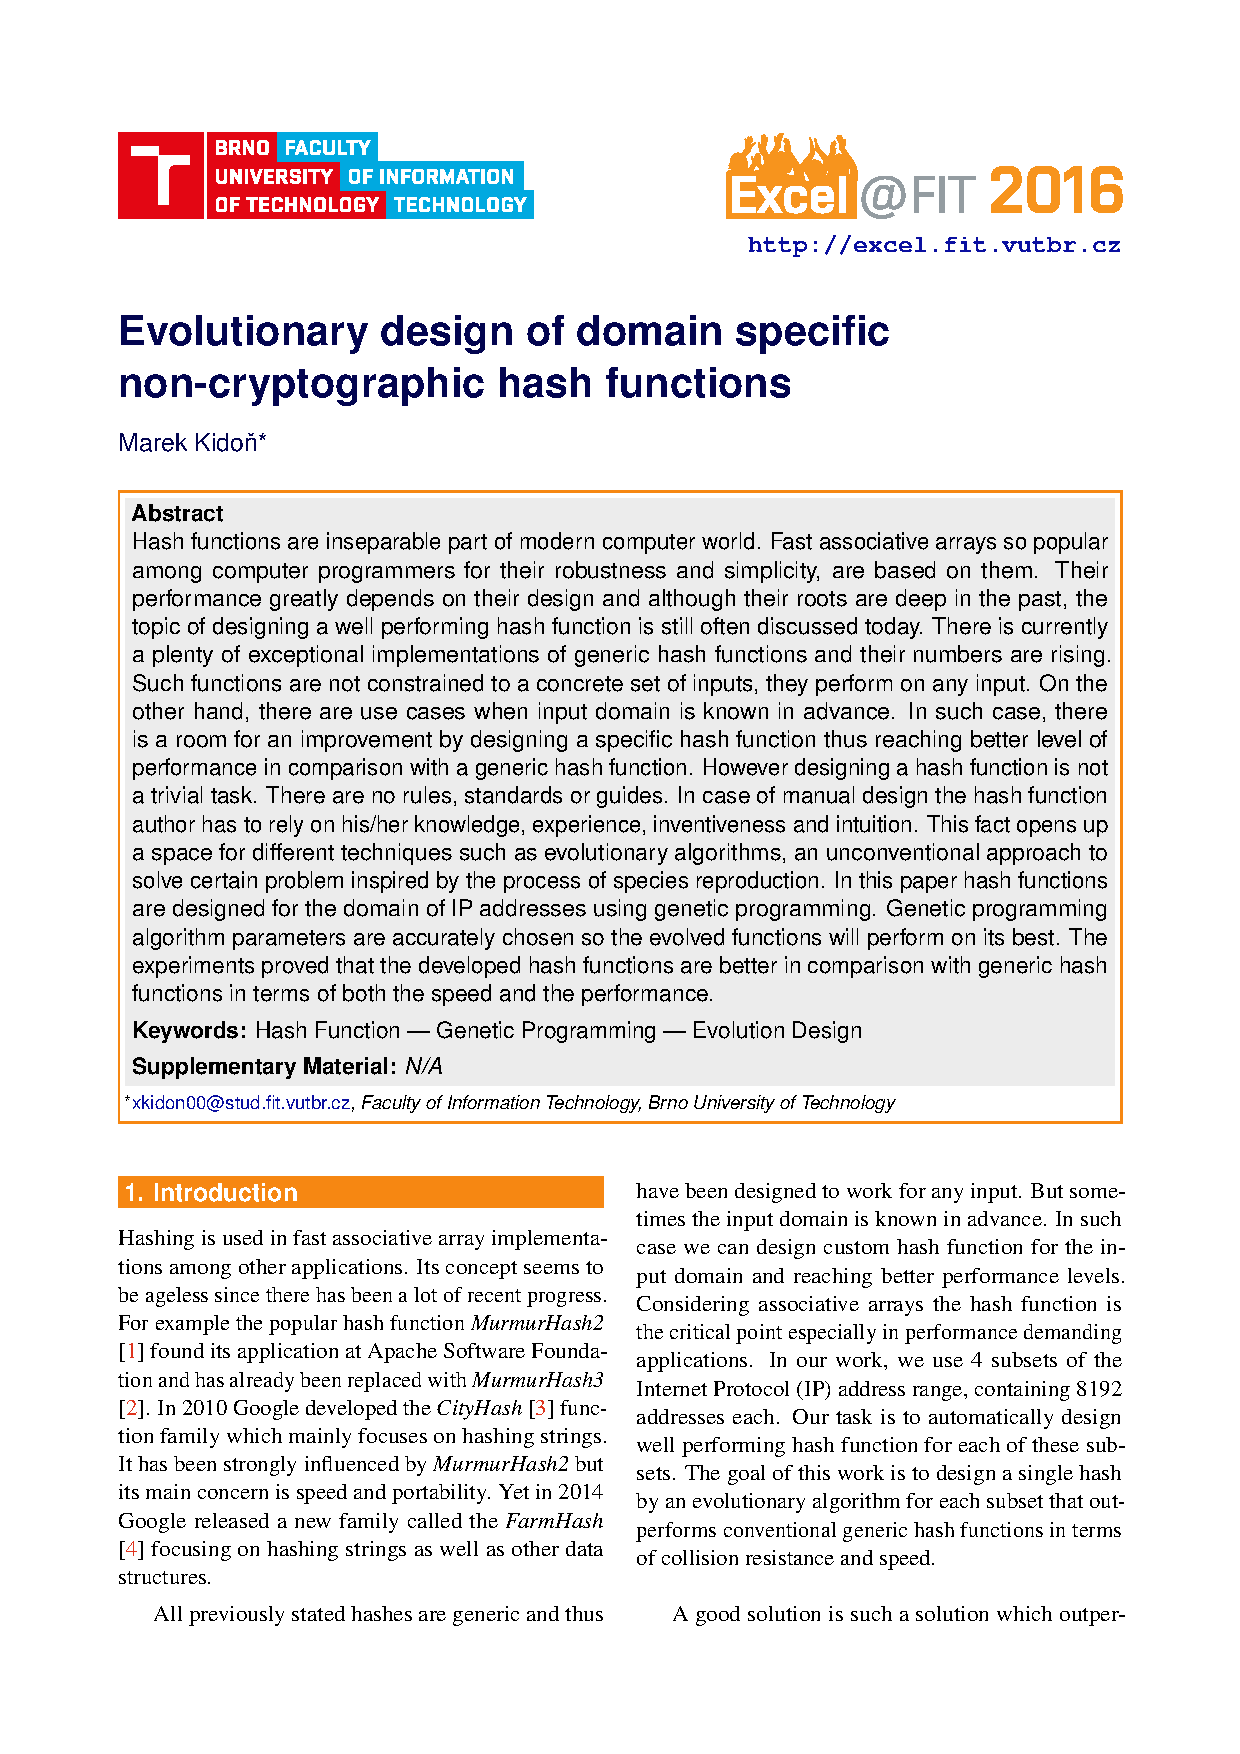
\includepdf[pages=1]{includes/ExcelFITPaper.pdf}
\end{figure}
\newpage
\begin{figure}[!ht]
	\centering 
	\includepdf[pages=2]{includes/ExcelFITPaper.pdf}
\end{figure}
\newpage
\begin{figure}[!ht]
	\centering 
	\includepdf[pages=3]{includes/ExcelFITPaper.pdf}
\end{figure}
\newpage
\begin{figure}[!ht]
	\centering 
	\includepdf[pages=4]{includes/ExcelFITPaper.pdf}
\end{figure}
\newpage
\begin{figure}[!ht]
	\centering 
	\includepdf[pages=5]{includes/ExcelFITPaper.pdf}
\end{figure}
\newpage
\begin{figure}[!ht]
	\centering 
	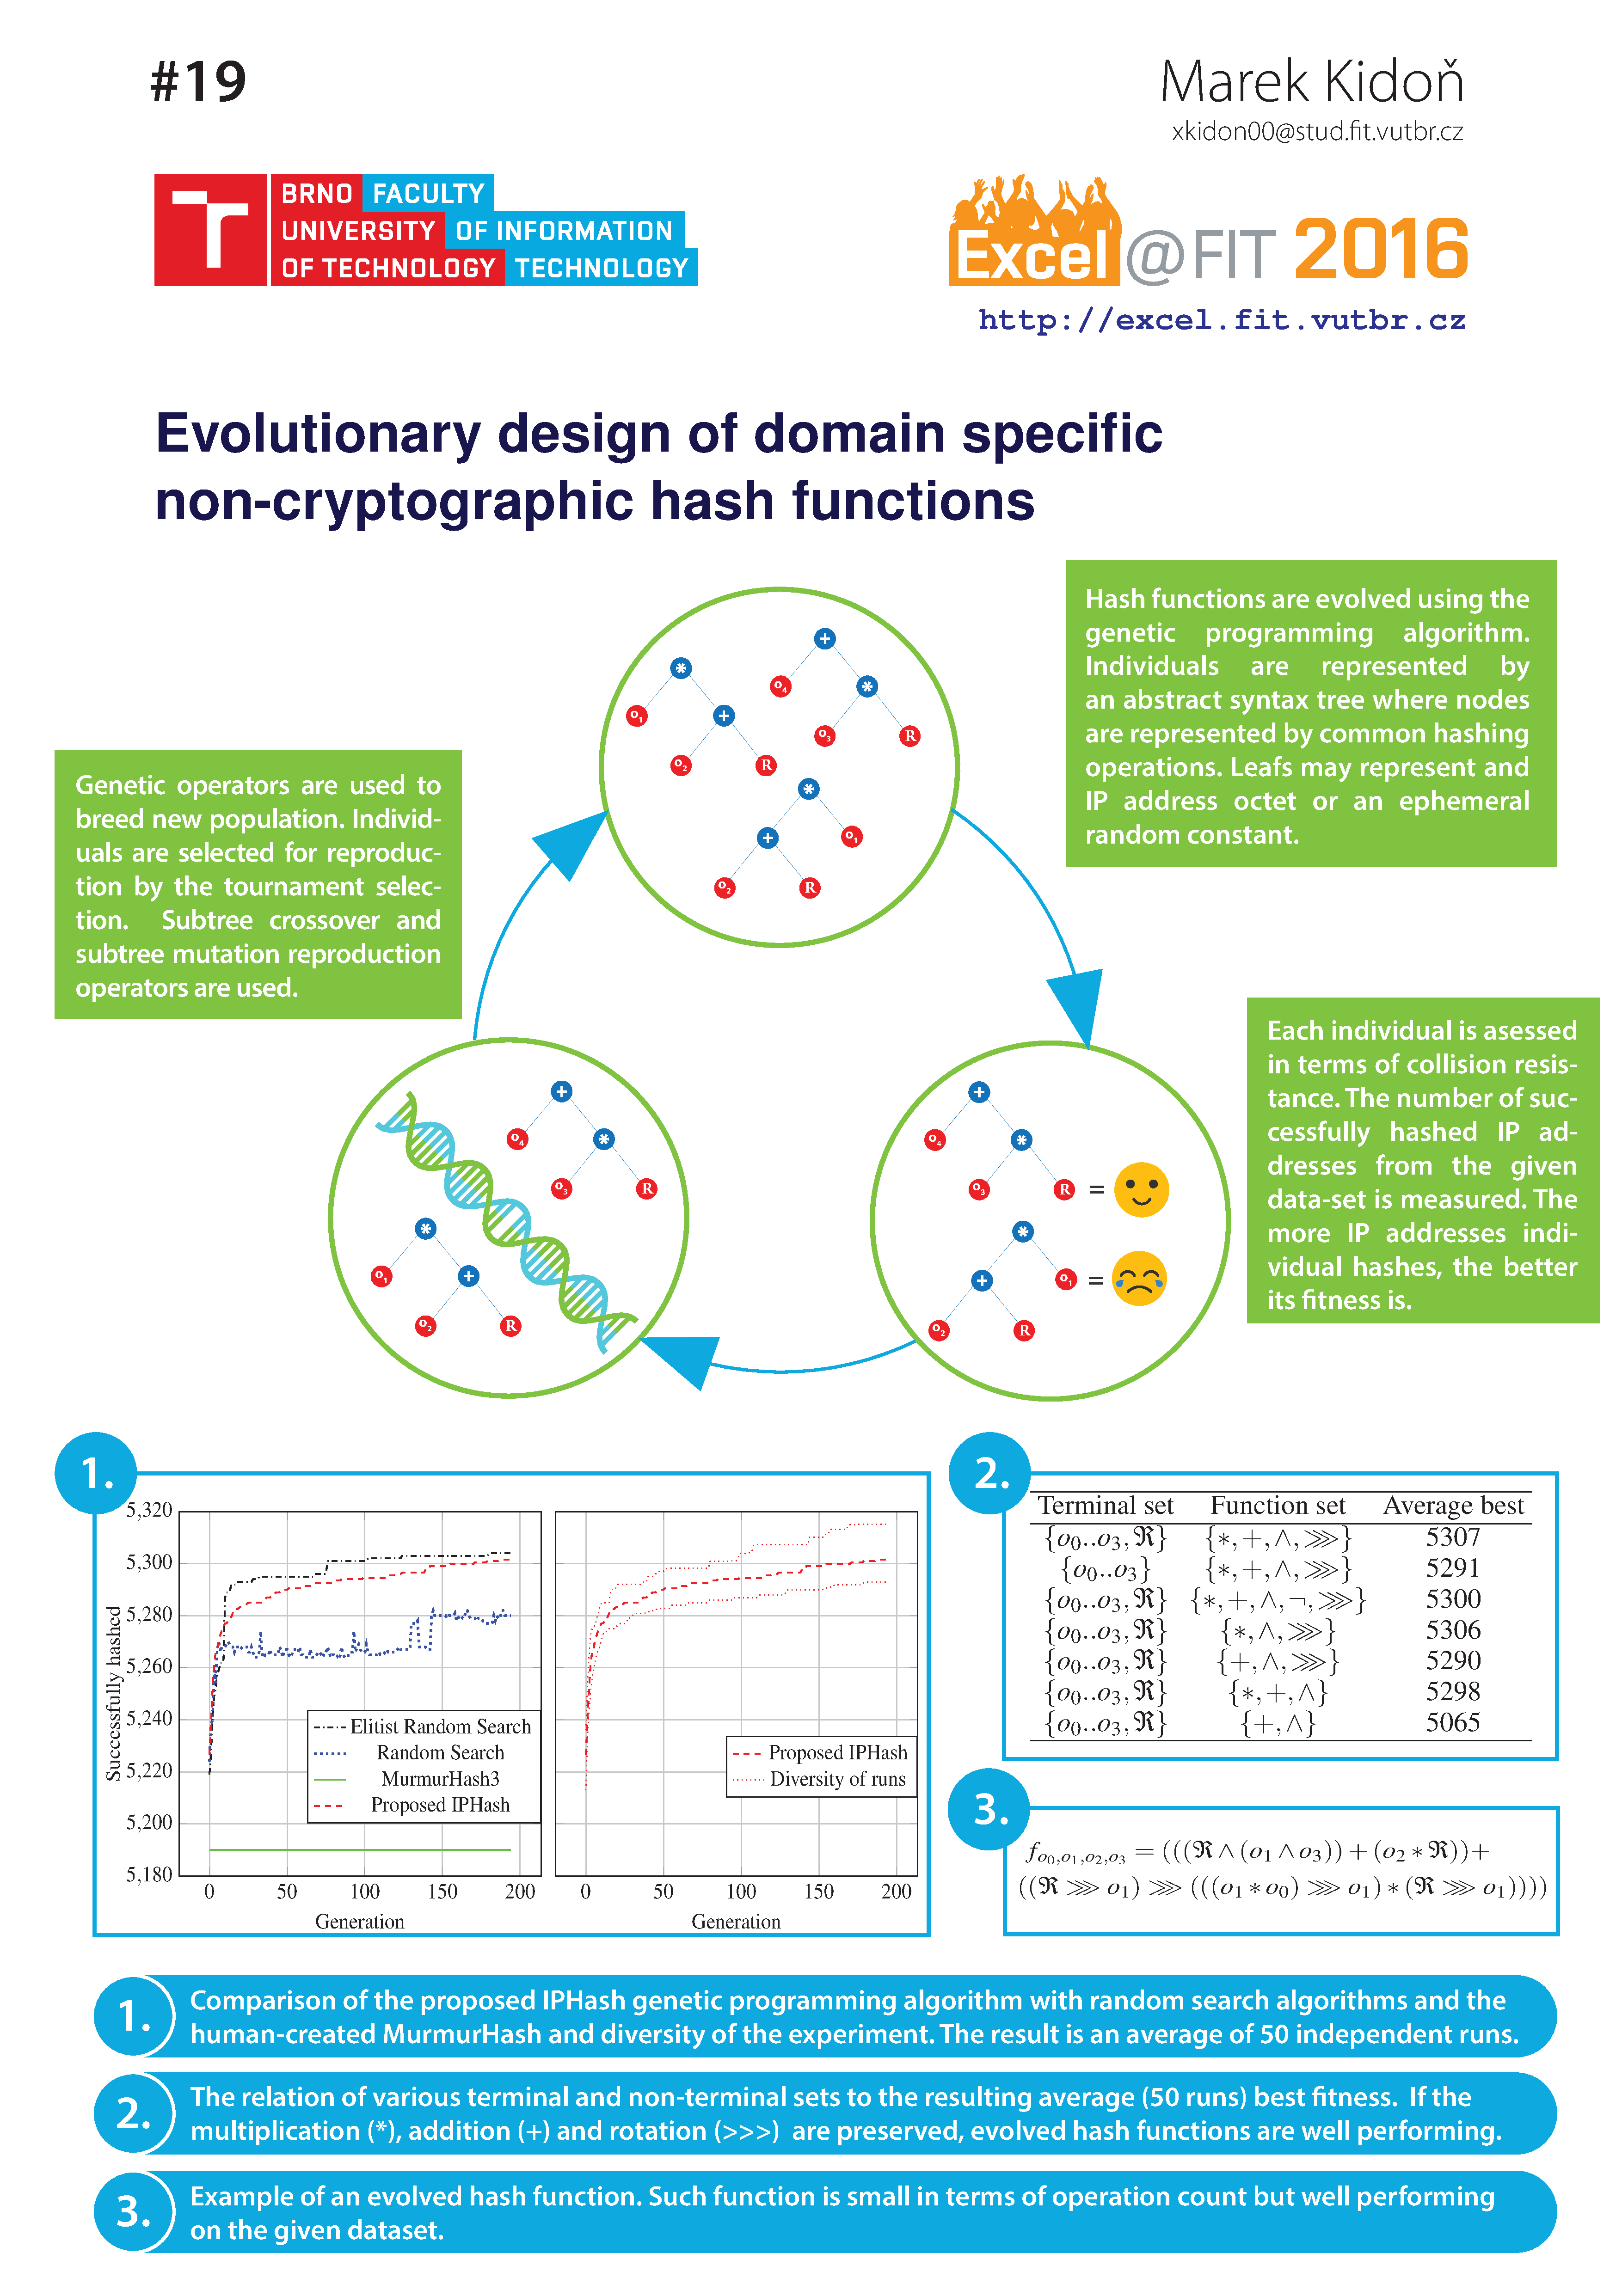
\includepdf{includes/ExcelFITPoster.pdf}
\end{figure}

 % viz. prilohy.tex
\end{document}
